\documentclass[10pt, a4paper]{book}
\renewcommand\familydefault{\sfdefault}

%%%%%%%%%%%%%%%%%%%%%%%%%%%%%%%%%%%%%%%%%
% The Legrand Orange Book
% Structural Definitions File
% Version 2.0 (9/2/15)
%
% Original author:
% Mathias Legrand (legrand.mathias@gmail.com) with modifications by:
% Vel (vel@latextemplates.com)
% 
% This file has been downloaded from:
% http://www.LaTeXTemplates.com
%
% License:
% CC BY-NC-SA 3.0 (http://creativecommons.org/licenses/by-nc-sa/3.0/)
%
%%%%%%%%%%%%%%%%%%%%%%%%%%%%%%%%%%%%%%%%%

%----------------------------------------------------------------------------------------
%	VARIOUS REQUIRED PACKAGES AND CONFIGURATIONS
%----------------------------------------------------------------------------------------

\usepackage[top=2.0cm,bottom=2.0cm,left=2.5cm,right=2cm,headsep=10pt,a4paper]{geometry} % Page margins

\usepackage{graphicx} % Required for including pictures
\graphicspath{{Pictures/}} % Specifies the directory where pictures are stored

\usepackage{lipsum} % Inserts dummy text

\usepackage{tikz} % Required for drawing custom shapes

\usepackage[english]{babel} % English language/hyphenation

\usepackage{enumitem} % Customize lists
\setlist{nolistsep} % Reduce spacing between bullet points and numbered lists

\usepackage{booktabs} % Required for nicer horizontal rules in tables

\usepackage{xcolor} % Required for specifying colors by name
% \definecolor{ocre}{RGB}{45,74,110} % Define the orange color used for highlighting throughout the book
\definecolor{ocre}{HTML}{3F729B}

%----------------------------------------------------------------------------------------
%	FONTS
%----------------------------------------------------------------------------------------

\usepackage{avant} % Use the Avantgarde font for headings
%\usepackage{times} % Use the Times font for headings
\usepackage{mathptmx} % Use the Adobe Times Roman as the default text font together with math symbols from the Sym­bol, Chancery and Com­puter Modern fonts

\usepackage{microtype} % Slightly tweak font spacing for aesthetics
\usepackage[utf8]{inputenc} % Required for including letters with accents
\usepackage[T1]{fontenc} % Use 8-bit encoding that has 256 glyphs

%----------------------------------------------------------------------------------------
%	BIBLIOGRAPHY AND INDEX
%----------------------------------------------------------------------------------------

\usepackage[style=alphabetic,citestyle=numeric,sorting=nyt,sortcites=true,autopunct=true,hyperref=true,abbreviate=false,backend=biber]{biblatex}
\addbibresource{bibliography.bib} % BibTeX bibliography file
\defbibheading{bibempty}{}

\usepackage{calc} % For simpler calculation - used for spacing the index letter headings correctly
\usepackage{makeidx} % Required to make an index
\makeindex % Tells LaTeX to create the files required for indexing

%----------------------------------------------------------------------------------------
%	MAIN TABLE OF CONTENTS
%----------------------------------------------------------------------------------------

\usepackage{titletoc} % Required for manipulating the table of contents

\contentsmargin{0cm} % Removes the default margin

% Part text styling
\titlecontents{part}[0cm]
{\addvspace{20pt}\centering\large\bfseries}
{}
{}
{}

% Chapter text styling
\titlecontents{chapter}[1.25cm] % Indentation
{\addvspace{12pt}\large\sffamily\bfseries} % Spacing and font options for chapters
{\color{ocre!60}\contentslabel[\Large\thecontentslabel]{1.25cm}\color{ocre}} % Chapter number
{\color{ocre}}  
{\color{ocre!60}\normalsize\;\titlerule*[.5pc]{.}\;\thecontentspage} % Page number

% Section text styling
\titlecontents{section}[1.25cm] % Indentation
{\addvspace{3pt}\sffamily\bfseries} % Spacing and font options for sections
{\contentslabel[\thecontentslabel]{1.25cm}} % Section number
{}
{\hfill\color{black}\thecontentspage} % Page number
[]

% Subsection text styling
\titlecontents{subsection}[1.25cm] % Indentation
{\addvspace{1pt}\sffamily\small} % Spacing and font options for subsections
{\contentslabel[\thecontentslabel]{1.25cm}} % Subsection number
{}
{\ \titlerule*[.5pc]{.}\;\thecontentspage} % Page number
[]

% List of figures
\titlecontents{figure}[0em]
{\addvspace{-5pt}\sffamily}
{\thecontentslabel\hspace*{1em}}
{}
{\ \titlerule*[.5pc]{.}\;\thecontentspage}
[]

% List of tables
\titlecontents{table}[0em]
{\addvspace{-5pt}\sffamily}
{\thecontentslabel\hspace*{1em}}
{}
{\ \titlerule*[.5pc]{.}\;\thecontentspage}
[]

%----------------------------------------------------------------------------------------
%	MINI TABLE OF CONTENTS IN PART HEADS
%----------------------------------------------------------------------------------------

% Chapter text styling
\titlecontents{lchapter}[0em] % Indenting
{\addvspace{15pt}\large\sffamily\bfseries} % Spacing and font options for chapters
{\color{ocre}\contentslabel[\Large\thecontentslabel]{1.25cm}\color{ocre}} % Chapter number
{}  
{\color{ocre}\normalsize\sffamily\bfseries\;\titlerule*[.5pc]{.}\;\thecontentspage} % Page number

% Section text styling
\titlecontents{lsection}[0em] % Indenting
{\sffamily\small} % Spacing and font options for sections
{\contentslabel[\thecontentslabel]{1.25cm}} % Section number
{}
{}

% Subsection text styling
\titlecontents{lsubsection}[.5em] % Indentation
{\normalfont\footnotesize\sffamily} % Font settings
{}
{}
{}

%----------------------------------------------------------------------------------------
%	PAGE HEADERS
%----------------------------------------------------------------------------------------

\usepackage{fancyhdr} % Required for header and footer configuration

\pagestyle{fancy}
\renewcommand{\chaptermark}[1]{\markboth{\sffamily\normalsize\bfseries\chaptername\ \thechapter.\ #1}{}} % Chapter text font settings
\renewcommand{\sectionmark}[1]{\markright{\sffamily\normalsize\thesection\hspace{5pt}#1}{}} % Section text font settings
\fancyhf{} \fancyhead[LE,RO]{\sffamily\normalsize\thepage} % Font setting for the page number in the header
\fancyhead[LO]{\rightmark} % Print the nearest section name on the left side of odd pages
\fancyhead[RE]{\leftmark} % Print the current chapter name on the right side of even pages
\renewcommand{\headrulewidth}{0.5pt} % Width of the rule under the header
\addtolength{\headheight}{2.5pt} % Increase the spacing around the header slightly
\renewcommand{\footrulewidth}{0pt} % Removes the rule in the footer
\fancypagestyle{plain}{\fancyhead{}\renewcommand{\headrulewidth}{0pt}} % Style for when a plain pagestyle is specified

% Removes the header from odd empty pages at the end of chapters
\makeatletter
\renewcommand{\cleardoublepage}{
\clearpage\ifodd\c@page\else
\hbox{}
\vspace*{\fill}
\thispagestyle{empty}
\newpage
\fi}

%----------------------------------------------------------------------------------------
%	THEOREM STYLES
%----------------------------------------------------------------------------------------

\usepackage{amsmath,amsfonts,amssymb,amsthm} % For math equations, theorems, symbols, etc

\newcommand{\intoo}[2]{\mathopen{]}#1\,;#2\mathclose{[}}
\newcommand{\ud}{\mathop{\mathrm{{}d}}\mathopen{}}
\newcommand{\intff}[2]{\mathopen{[}#1\,;#2\mathclose{]}}
\newtheorem{notation}{Notation}[chapter]

% Boxed/framed environments
\newtheoremstyle{ocrenumbox}% % Theorem style name
{0pt}% Space above
{0pt}% Space below
{\normalfont}% % Body font
{}% Indent amount
{\small\bf\sffamily\color{ocre}}% % Theorem head font
{\;}% Punctuation after theorem head
{0.25em}% Space after theorem head
{\small\sffamily\color{ocre}\thmname{#1}\nobreakspace\thmnumber{\@ifnotempty{#1}{}\@upn{#2}}% Theorem text (e.g. Theorem 2.1)
\thmnote{\nobreakspace\the\thm@notefont\sffamily\bfseries\color{black}---\nobreakspace#3.}} % Optional theorem note
\renewcommand{\qedsymbol}{$\blacksquare$}% Optional qed square

\newtheoremstyle{blacknumex}% Theorem style name
{5pt}% Space above
{5pt}% Space below
{\normalfont}% Body font
{} % Indent amount
{\small\bf\sffamily}% Theorem head font
{\;}% Punctuation after theorem head
{0.25em}% Space after theorem head
{\small\sffamily{\tiny\ensuremath{\blacksquare}}\nobreakspace\thmname{#1}\nobreakspace\thmnumber{\@ifnotempty{#1}{}\@upn{#2}}% Theorem text (e.g. Theorem 2.1)
\thmnote{\nobreakspace\the\thm@notefont\sffamily\bfseries---\nobreakspace#3.}}% Optional theorem note

\newtheoremstyle{blacknumbox} % Theorem style name
{0pt}% Space above
{0pt}% Space below
{\normalfont}% Body font
{}% Indent amount
{\small\bf\sffamily}% Theorem head font
{\;}% Punctuation after theorem head
{0.25em}% Space after theorem head
{\small\sffamily\thmname{#1}\nobreakspace\thmnumber{\@ifnotempty{#1}{}\@upn{#2}}% Theorem text (e.g. Theorem 2.1)
\thmnote{\nobreakspace\the\thm@notefont\sffamily\bfseries---\nobreakspace#3.}}% Optional theorem note

% Non-boxed/non-framed environments
\newtheoremstyle{ocrenum}% % Theorem style name
{5pt}% Space above
{5pt}% Space below
{\normalfont}% % Body font
{}% Indent amount
{\small\bf\sffamily\color{ocre}}% % Theorem head font
{\;}% Punctuation after theorem head
{0.25em}% Space after theorem head
{\small\sffamily\color{ocre}\thmname{#1}\nobreakspace\thmnumber{\@ifnotempty{#1}{}\@upn{#2}}% Theorem text (e.g. Theorem 2.1)
\thmnote{\nobreakspace\the\thm@notefont\sffamily\bfseries\color{black}---\nobreakspace#3.}} % Optional theorem note
\renewcommand{\qedsymbol}{$\blacksquare$}% Optional qed square
\makeatother

% Defines the theorem text style for each type of theorem to one of the three styles above
\newcounter{dummy} 
\numberwithin{dummy}{section}
\theoremstyle{ocrenumbox}
\newtheorem{theoremeT}[dummy]{Theorem}
\newtheorem{problem}{Problem}[chapter]
\newtheorem{exerciseT}{Exercise}[chapter]
\theoremstyle{blacknumex}
\newtheorem{exampleT}{Example}[chapter]
\theoremstyle{blacknumbox}
\newtheorem{vocabulary}{Vocabulary}[chapter]
\newtheorem{definitionT}{Definition}[section]
\newtheorem{corollaryT}[dummy]{Corollary}
\theoremstyle{ocrenum}
\newtheorem{proposition}[dummy]{Proposition}

%----------------------------------------------------------------------------------------
%	DEFINITION OF COLORED BOXES
%----------------------------------------------------------------------------------------

\RequirePackage[framemethod=default]{mdframed} % Required for creating the theorem, definition, exercise and corollary boxes

% Theorem box
\newmdenv[skipabove=7pt,
skipbelow=7pt,
backgroundcolor=black!5,
linecolor=ocre,
innerleftmargin=5pt,
innerrightmargin=5pt,
innertopmargin=5pt,
leftmargin=0cm,
rightmargin=0cm,
innerbottommargin=5pt]{tBox}

% Exercise box	  
\newmdenv[skipabove=7pt,
skipbelow=7pt,
rightline=false,
leftline=true,
topline=false,
bottomline=false,
backgroundcolor=ocre!10,
linecolor=ocre,
innerleftmargin=5pt,
innerrightmargin=5pt,
innertopmargin=5pt,
innerbottommargin=5pt,
leftmargin=0cm,
rightmargin=0cm,
linewidth=4pt]{eBox}	

% Definition box
\newmdenv[skipabove=7pt,
skipbelow=7pt,
rightline=false,
leftline=true,
topline=false,
bottomline=false,
linecolor=ocre,
innerleftmargin=5pt,
innerrightmargin=5pt,
innertopmargin=0pt,
leftmargin=0cm,
rightmargin=0cm,
linewidth=4pt,
innerbottommargin=0pt]{dBox}	

% Corollary box
\newmdenv[skipabove=7pt,
skipbelow=7pt,
rightline=false,
leftline=true,
topline=false,
bottomline=false,
linecolor=gray,
backgroundcolor=black!5,
innerleftmargin=5pt,
innerrightmargin=5pt,
innertopmargin=5pt,
leftmargin=0cm,
rightmargin=0cm,
linewidth=4pt,
innerbottommargin=5pt]{cBox}

% Creates an environment for each type of theorem and assigns it a theorem text style from the "Theorem Styles" section above and a colored box from above
\newenvironment{theorem}{\begin{tBox}\begin{theoremeT}}{\end{theoremeT}\end{tBox}}
\newenvironment{exercise}{\begin{eBox}\begin{exerciseT}}{\hfill{\color{ocre}\tiny\ensuremath{\blacksquare}}\end{exerciseT}\end{eBox}}				  
\newenvironment{definition}{\begin{dBox}\begin{definitionT}}{\end{definitionT}\end{dBox}}	
\newenvironment{example}{\begin{exampleT}}{\hfill{\tiny\ensuremath{\blacksquare}}\end{exampleT}}		
\newenvironment{corollary}{\begin{cBox}\begin{corollaryT}}{\end{corollaryT}\end{cBox}}	

%----------------------------------------------------------------------------------------
%	REMARK ENVIRONMENT
%----------------------------------------------------------------------------------------

\newenvironment{remark}{\par\vspace{10pt}\small % Vertical white space above the remark and smaller font size
\begin{list}{}{
\leftmargin=35pt % Indentation on the left
\rightmargin=25pt}\item\ignorespaces % Indentation on the right
\makebox[-2.5pt]{\begin{tikzpicture}[overlay]
\node[draw=ocre!60,line width=1pt,circle,fill=ocre!25,font=\sffamily\bfseries,inner sep=2pt,outer sep=0pt] at (-15pt,0pt){\textcolor{ocre}{R}};\end{tikzpicture}} % Orange R in a circle
\advance\baselineskip -1pt}{\end{list}\vskip5pt} % Tighter line spacing and white space after remark

%----------------------------------------------------------------------------------------
%	SECTION NUMBERING IN THE MARGIN
%----------------------------------------------------------------------------------------

\makeatletter
\renewcommand{\@seccntformat}[1]{\llap{\textcolor{ocre}{\csname the#1\endcsname}\hspace{1em}}}                    
\renewcommand{\section}{\@startsection{section}{1}{\z@}
{-4ex \@plus -1ex \@minus -.4ex}
{1ex \@plus.2ex }
{\normalfont\large\sffamily\bfseries}}
\renewcommand{\subsection}{\@startsection {subsection}{2}{\z@}
{-3ex \@plus -0.1ex \@minus -.4ex}
{0.5ex \@plus.2ex }
{\normalfont\sffamily\bfseries}}
\renewcommand{\subsubsection}{\@startsection {subsubsection}{3}{\z@}
{-2ex \@plus -0.1ex \@minus -.2ex}
{.2ex \@plus.2ex }
{\normalfont\small\sffamily\bfseries}}                        
\renewcommand\paragraph{\@startsection{paragraph}{4}{\z@}
{-2ex \@plus-.2ex \@minus .2ex}
{.1ex}
{\normalfont\small\sffamily\bfseries}}

%----------------------------------------------------------------------------------------
%	PART HEADINGS
%----------------------------------------------------------------------------------------

% numbered part in the table of contents
\newcommand{\@mypartnumtocformat}[2]{%
\setlength\fboxsep{0pt}%
\noindent\colorbox{ocre!20}{\strut\parbox[c][.7cm]{\ecart}{\color{ocre!70}\Large\sffamily\bfseries\centering#1}}\hskip\esp\colorbox{ocre!40}{\strut\parbox[c][.7cm]{\linewidth-\ecart-\esp}{\Large\sffamily\centering#2}}}%
%%%%%%%%%%%%%%%%%%%%%%%%%%%%%%%%%%
% unnumbered part in the table of contents
\newcommand{\@myparttocformat}[1]{%
\setlength\fboxsep{0pt}%
\noindent\colorbox{ocre!40}{\strut\parbox[c][.7cm]{\linewidth}{\Large\sffamily\centering#1}}}%
%%%%%%%%%%%%%%%%%%%%%%%%%%%%%%%%%%
\newlength\esp
\setlength\esp{4pt}
\newlength\ecart
\setlength\ecart{1.2cm-\esp}
\newcommand{\thepartimage}{}%
\newcommand{\partimage}[1]{\renewcommand{\thepartimage}{#1}}%
\def\@part[#1]#2{%
\ifnum \c@secnumdepth >-2\relax%
\refstepcounter{part}%
\addcontentsline{toc}{part}{\texorpdfstring{\protect\@mypartnumtocformat{\thepart}{#1}}{\partname~\thepart\ ---\ #1}}
\else%
\addcontentsline{toc}{part}{\texorpdfstring{\protect\@myparttocformat{#1}}{#1}}%
\fi%
\startcontents%
\markboth{}{}%
{\thispagestyle{empty}%
\begin{tikzpicture}[remember picture,overlay]%
\node at (current page.north west){\begin{tikzpicture}[remember picture,overlay]%	
\fill[ocre!20](0cm,0cm) rectangle (\paperwidth,-\paperheight);
\node[anchor=north] at (4cm,-3.25cm){\color{ocre!40}\fontsize{220}{100}\sffamily\bfseries\thepart}; 
\node[anchor=south east] at (\paperwidth-1cm,-\paperheight+1cm){\parbox[t][][t]{8.5cm}{
\printcontents{l}{0}{\setcounter{tocdepth}{1}}%
}};
\node[anchor=north east] at (\paperwidth-1.5cm,-3.25cm){\parbox[t][][t]{15cm}{\strut\raggedleft\color{white}\fontsize{30}{30}\sffamily\bfseries#2}};
\end{tikzpicture}};
\end{tikzpicture}}%
\@endpart}
\def\@spart#1{%
\startcontents%
\phantomsection
{\thispagestyle{empty}%
\begin{tikzpicture}[remember picture,overlay]%
\node at (current page.north west){\begin{tikzpicture}[remember picture,overlay]%	
\fill[ocre!20](0cm,0cm) rectangle (\paperwidth,-\paperheight);
\node[anchor=north east] at (\paperwidth-1.5cm,-3.25cm){\parbox[t][][t]{15cm}{\strut\raggedleft\color{white}\fontsize{30}{30}\sffamily\bfseries#1}};
\end{tikzpicture}};
\end{tikzpicture}}
\addcontentsline{toc}{part}{\texorpdfstring{%
\setlength\fboxsep{0pt}%
\noindent\protect\colorbox{ocre!40}{\strut\protect\parbox[c][.7cm]{\linewidth}{\Large\sffamily\protect\centering #1\quad\mbox{}}}}{#1}}%
\@endpart}
\def\@endpart{\vfil\newpage
\if@twoside
\if@openright
\null
\thispagestyle{empty}%
\newpage
\fi
\fi
\if@tempswa
\twocolumn
\fi}

%----------------------------------------------------------------------------------------
%	CHAPTER HEADINGS
%----------------------------------------------------------------------------------------

% A switch to conditionally include a picture, implemented by  Christian Hupfer
\newif\ifusechapterimage
\usechapterimagetrue
\newcommand{\thechapterimage}{}%
\newcommand{\chapterimage}[1]{\ifusechapterimage\renewcommand{\thechapterimage}{#1}\fi}%
\newcommand{\autodot}{.}
\def\@makechapterhead#1{%
{\parindent \z@ \raggedright \normalfont
\ifnum \c@secnumdepth >\m@ne
\if@mainmatter
\begin{tikzpicture}[remember picture,overlay]
\node at (current page.north west)
{\begin{tikzpicture}[remember picture,overlay]
\node[anchor=north west,inner sep=0pt] at (0,0) {\ifusechapterimage\includegraphics[width=\paperwidth]{\thechapterimage}\fi};
\draw[anchor=west] (\Gm@lmargin,-9cm) node [line width=2pt,rounded corners=15pt,draw=ocre,fill=white,fill opacity=0.5,inner sep=15pt]{\strut\makebox[22cm]{}};
\draw[anchor=west] (\Gm@lmargin+.3cm,-9cm) node {\huge\sffamily\bfseries\color{black}\thechapter\autodot~#1\strut};
\end{tikzpicture}};
\end{tikzpicture}
\else
\begin{tikzpicture}[remember picture,overlay]
\node at (current page.north west)
{\begin{tikzpicture}[remember picture,overlay]
\node[anchor=north west,inner sep=0pt] at (0,0) {\ifusechapterimage\includegraphics[width=\paperwidth]{\thechapterimage}\fi};
\draw[anchor=west] (\Gm@lmargin,-9cm) node [line width=2pt,rounded corners=15pt,draw=ocre,fill=white,fill opacity=0.5,inner sep=15pt]{\strut\makebox[22cm]{}};
\draw[anchor=west] (\Gm@lmargin+.3cm,-9cm) node {\huge\sffamily\bfseries\color{black}#1\strut};
\end{tikzpicture}};
\end{tikzpicture}
\fi\fi\par\vspace*{270\p@}}}

%-------------------------------------------
% PIETRO
%-------------------------------------------

\def\@makeschapterhead#1{%
\begin{tikzpicture}[remember picture,overlay]
\node at (current page.north west)
{\begin{tikzpicture}[remember picture,overlay]
\node[anchor=north west,inner sep=0pt] at (0,0) {\ifusechapterimage\includegraphics[width=\paperwidth]{\thechapterimage}\fi};
\draw[anchor=west] (\Gm@lmargin,-9cm) node [line width=2pt,rounded corners=15pt,draw=ocre,fill=white,fill opacity=0.5,inner sep=15pt]{\strut\makebox[22cm]{}};
\draw[anchor=west] (\Gm@lmargin+.3cm,-9cm) node {\huge\sffamily\bfseries\color{black}#1\strut};
\end{tikzpicture}};
\end{tikzpicture}
\par\vspace*{270\p@}}
\makeatother

%----------------------------------------------------------------------------------------
%	HYPERLINKS IN THE DOCUMENTS
%----------------------------------------------------------------------------------------

\usepackage{hyperref}
\hypersetup{hidelinks,colorlinks=false,breaklinks=true,urlcolor= ocre,bookmarksopen=false,pdftitle={Title},pdfauthor={Author}}
\usepackage{bookmark}
\bookmarksetup{
open,
numbered,
addtohook={%
\ifnum\bookmarkget{level}=0 % chapter
\bookmarksetup{bold}%
\fi
\ifnum\bookmarkget{level}=-1 % part
\bookmarksetup{color=ocre,bold}%
\fi
}
}
 % Insert the commands.tex file which contains the majority of the structure behind the template
\usepackage{multicol}
\usepackage{wrapfig}
\newcommand{\mail}[1]{\href{mailto:#1}{\texttt{#1}}}
\newcommand{\member}[2]{{\textbf{#1}\\}{#2}}
\newcommand{\myaut}[1]{{\underline{#1}}}

%\setlength{\columnseprule}{0.5pt}
%\newcommand{\mail}[1]{\href{mailto:#1}{\texttt{#1}}}
%\newcommand{\member}[2]{{\textbf{#1}\\}{#2}}
%\newcommand{\myaut}[1]{{\underline{#1}}}

\hyphenation{aspects}

\begin{document}

\begingroup
\thispagestyle{empty}
\begin{tikzpicture}[remember picture,overlay]
\coordinate [below=12cm] (midpoint) at (current page.north);
\node at (current page.north west)
{\begin{tikzpicture}[remember picture,overlay]
\node[anchor=north west,inner sep=0pt] at (0,0) {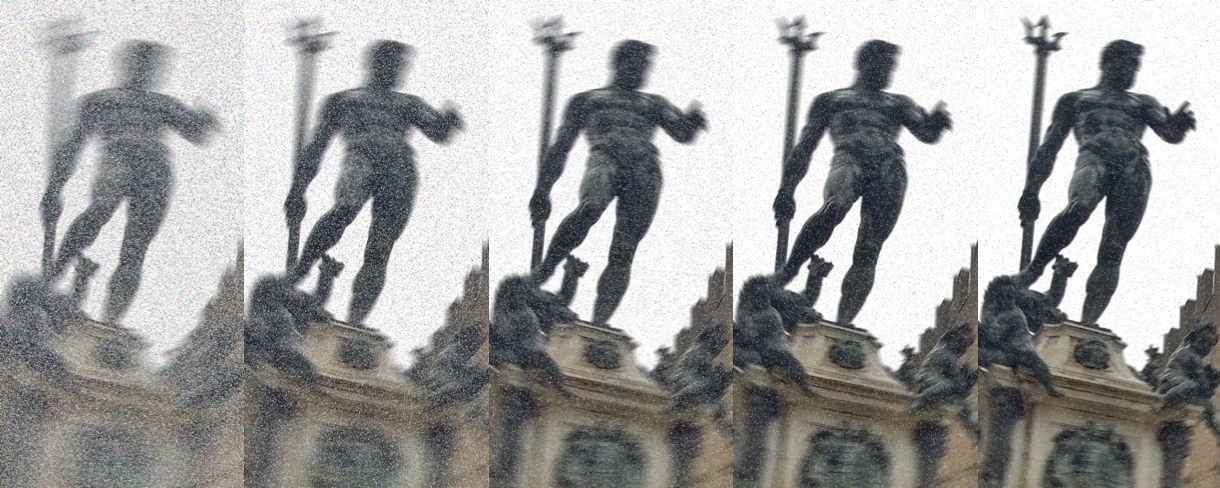
\includegraphics[width=\paperwidth]{images/nettuni.png}}; % Background
\draw[anchor=north] (midpoint) node [fill=myblue!30!white,fill opacity=0.6,text opacity=1,inner sep=1cm]{\Huge\centering\bfseries\sffamily\parbox[c][][t]{\paperwidth}{\centering SIAM Conference on IMAGING SCIENCE\\ Program and Abstracts\\[15pt] % Book title
{\Large June 5-8, 2018}\\[20pt] % Subtitle
{\huge University of Bologna, Italy}}}; % Author name
\end{tikzpicture}};
\end{tikzpicture}
\vfill
\endgroup
%\maketitle

%----------------------------------------------------------------------------------------
%	CONFERENCE THEMES
%----------------------------------------------------------------------------------------

\newpage
~\vfill
\thispagestyle{empty}

\noindent \textsc{https://siam-is18.dm.unibo.it}

\bigskip

\noindent This conference is the biennial activity of the SIAM Activity Group on Imaging Science.

\vspace{0.5cm}

\noindent The SIAM Activity Group on Imaging Science brings together SIAM members and other scientists and engineers with an interest 
in the mathematical and computational aspects of imaging.
The activity group organizes the biennial SIAM Conference on Imaging Science, awards the SIAG/IS Best Paper Prize
every two years to the authors of the best paper on mathematical and computational aspects of imaging, awards the SIAG/IS 
Early Career Prize to an outstanding early career researcher in the field of imaging science, and maintains a wiki, a
member directory, and an electronic mailing list.

\newpage

\section*{Conference Themes}

Reconstruction, enhancement, segmentation, analysis, registration, compression, representation, tomography, machine learning and tracking of two and three dimensional images are vital to many areas of science, medicine, and engineering. The increasingly sophisticated mathematical, statistical and computational methods employed in these research areas are referred to as \emph{Imaging Science}.\\ 
These techniques include transform and orthogonal series methods, nonlinear optimization, numerical linear algebra, integral equations, partial differential equations, Bayesian and other statistical inverse estimation methods, operator theory, differential geometry, information theory, interpolation and approximation, inverse problems, computer graphics and vision, stochastic processes, and others.

\smallskip

SIAM-IS18 will exchange research results and address open issues in all aspects of imaging science
and provide a forum for the presentation of work in imaging science.



\section*{Committee}

\bigskip
\noindent \textbf{\color{siamblue}General Co-Chairs}
\bigskip

\begin{itemize}
  \item[] \member{Omar Ghattas}{University of Texas at Austin, USA}
  \item[] \member{Fiorella Sgallari}{University of Bologna}
\end{itemize}

\bigskip
\noindent \textbf{\color{siamblue}Scientific Committee}
\bigskip

\begin{itemize}
  \item[] \member{Marcelo Bertalm\'io}{University Pompeu Fabra, Spain}
  \item[] \member{Julianne Chung}{Virginia Tech., USA}
  \item[] \member{Per Christian Hansen}{Technical University of Denmark, Denmark }
  \item[] \member{Jari Kaipio}{University of Auckland, New Zealand}
  \item[] \member{Eric Miller}{Tufts University, USA}
  \item[] \member{Mila Nikolova}{CNRS ENS Cachan, France}
  \item[] \member{Ronny Ramlau}{Kepler University Linz, Austria and Johann Radon Institute, Austria}
  \item[] \member{Carola Sch\"{o}nlieb}{University of Cambridge, United Kingdom}
  \item[] \member{Gabriele Steidl}{Tech.Univ. Kaiserslautern, Germany}
  \item[] \member{Xue-Cheng Tai}{Hong Kong Baptist University, China }
  \item[] \member{Laura Waller}{University of California Berkeley, USA }
  \item[] \member{Brendt Wohlberg}{Los Alamos National Laboratory, USA}
\end{itemize}

\bigskip
\noindent\textbf{\color{siamblue}Organizing Committee}
\bigskip

\begin{itemize}
  \item[] \member{Carolina Beccari}{Dept. Mathematics, University of Bologna}
  \item[] \member{Giulio Casciola}{Dept. Mathematics, University of Bologna}
  \item[] \member{Salvatore Cuomo}{Dept. Mathematics and Applications ``Renato Caccioppoli'', University of Naples}
  \item[] \member{Luigi Di Stefano}{Dept. Computer Science and Engineering, University of Bologna}
  \item[] \member{Giovanni Dore}{Dept. Mathematics, University of Bologna}
  \item[] \member{Maurizio Falcone}{Dept. Mathematics, University of Roma ``La Sapienza''}
  \item[] \member{Luca Formaggia}{Department of Mathematics, Politecnico di Milano}
  \item[] \member{Patrizio Frosini}{Dept. Mathematics, University of Bologna}
  \item[] \member{Germana Landi,}{Dept. Mathematics, University of Bologna}
  \item[] \member{Alessandro Lanza}{Dept. Mathematics, University of Bologna}
  \item[] \member{Damiana Lazzaro}{Dept. Mathematics, University of Bologna}
  \item[] \member{Roberto Mecca}{University of Bologna and University of Cambridge}
  \item[] \member{Serena Morigi}{Dept. Mathematics, University of Bologna}
  \item[] \member{Michele Piana}{Dept. Mathematics, University of Genova}
  \item[] \member{Elena Loli Piccolomini}{Dept. Mathematics, University of Bologna}
  \item[] \member{Giulia Scalet}{Dept. Civil Engineering and Architecture, University of Pavia}
  \item[] \member{Federica Sciacchitano}{Dept. Mathematics, University of Genova}
  \item[] \member{Valeria Simoncini}{Dept. Mathematics, University of Bologna}
  \item[] \member{Giulia Spaletta}{Dept. Mathematics, University of Bologna}
  \item[] \member{Fabiana Zama}{Dept. Mathematics, University of Bologna}
\end{itemize}



%----------------------------------------------------------------------------------------
%	TABLE OF CONTENTS
%----------------------------------------------------------------------------------------

%\usechapterimagefalse % If you don't want to include a chapter image, use this to toggle images off - it can be enabled later with 
\usechapterimagetrue

\chapterimage{images/nettuni} % Table of contents heading image

\pagestyle{empty} % No headers

\tableofcontents % Print the table of contents itself

\cleardoublepage % Forces the first chapter to start on an odd page so it's on the right

\pagestyle{fancy} % Print headers again

%---------------At-A-GLANCE
%\newpage
%\section*{Program At-A-Glance}
%%\phantomsection
%\addcontentsline{toc}{section}{Program AT-A-Glance}


\newpage

%-----Registration Desk
\gisection{Registration Desk}
\addcontentsline{toc}{section}{Registration Desk}
The registration desk is located in the hall of Building A (via B. Andreatta 8) and is open during the following hours:

\bigskip

\begin{itemize}
  \item[] Monday, June 4: 3:00 PM - 6:30 PM
  \item[] Tuesday, June 5: 11:30 AM - 6:30 PM
  \item[] Wednesday, June 6: 8:00 AM - 6:30 PM
  \item[] Thursday, June 7: 8:00 AM - 1:30 PM
  \item[] Friday, June 8: 8:00 AM - 1:30 PM
\end{itemize}

%-----Badges
\gisection{Badges} 
Carry your badge during the conference so that you can be admitted to all technical sessions, coffee breaks, lunches, reception and banquet.\\
\textbf{Emergency numbers} are provided on the back of your name badge! 

%-----Registration Fee Includes
\gisection{Registration Fee Includes}

\bigskip

\begin{itemize}
  \item Admission to all technical sessions
  \item Business Meeting (open to SIAG/IS members)
  \item Social dinner (Wednesday)
  \item Coffee breaks 
  \item Welcome lunch (Tuesday)
  \item Welcome cocktail during the evening Poster Session (Tuesday)
  \item Room set-ups and audio/visual equipment
  \item Wi-Fi access at the conference
\end{itemize}%-----Conference Talk Arrangements

%-----Conference Talk Arrangements

\gisection{Conference Talk Arrangements}

\noindent All \textbf{plenary talks} will have a slot of 45 minutes
(5 minutes reserved for questions and discussion included).\\\\
The \textbf{minitutorials} will last 2 hours.\\\\
All \textbf{minisymposia talks} will have a slot of 30 minutes (5 minutes reserved for questions and discussion included).\\
All \textbf{contributed talks} will last 20 minutes (5 minutes reserved for questions and discussion included).\\\\
If you need to copy your presentation slides from your USB to a computer in lecture hall or meeting room, please do it in advance before
the session starts.

%-----Important Notice to Poster Presenters
\gisection{Important Notice to Poster Presenters}

\noindent The \textbf{poster sessions} are scheduled:
\begin{center}
  \textbf{Tuesday, June 5} \\
  from 6:30 PM onwards \\
  in Building A and B\\
  with Welcome cocktail

  \bigskip
   
  \textbf{Wednesday, June 6} \\
  from 11:30 AM to 1:00 PM \\
  in Building A and B
\end{center}

\noindent The \textbf{Best Poster Award} will be given on Friday, June 8 at 1:00 PM in Building A, Room A.\\

\noindent All posters participating to the Best Poster Award are available on the Conference website from June 1.\\
Poster presenters are requested to set up
their material on the provided poster boards (70 cm x 100 cm), following the instructions in the participant folder and be present during both sessions.  
All materials must be posted by Tuesday, June 5 at 6:00 PM.
The conference is not responsible for discarded posters.

%------------Wi-Fi Access
\gisection{Wi-Fi Access}
The username and password of your account during the conference period (5-8 June) can be found in your folder.

%-------------------Standard Audio/VIsual Set-Up in Meeting Rooms
\gisection{Standard Audio/Visual Set-Up in Meeting Rooms}
The plenary session room has a PC, two screens and two data projectors.\\ 
All other concurrent/breakout rooms have a PC, a screen, a data projector and a whiteboard (overhead projectors are also available).\\
The data projectors support VGA connection only. Presenters requiring an HDMI or alternate connection must provide their own adaptor.\\
Cables or adaptors for Apple computers are not supplied, as they vary for each model: please bring your own cable/adaptor if using a Mac computer. 
The conference is not responsible for the safety and security of speakers' computers.

%-------------Recording of presentations
\gisection{Presentations Recording}
During the conference audio and video recording is prohibited without the written permission of the speaker and the conference organizers.

%-------------SIAM Books and Journal
\gisection{SIAM Books and Journals}
%Display copies of books and complimentary copies of journals are available on site. SIAM books are available at a discounted price during the conference. The book booth will be staffed from 9:00 AM through 6:00 PM. \\If a SIAM books representative is temporarily away from the booth, completed order forms and payment (credit cards are preferred) may be taken to the registration desk. The books table will close at 4:00 PM on Friday??? (2016)\\
%Completed order forms should be emailed or faxed to the SIAM office directly. It is not allowed to carry out on site transaction during the conference period??? (2014)


\noindent Display copies of selected SIAM books are available on site.

\bigskip

\noindent SIAM books are offered at \textbf{discounted prices} for all attendees. 
SIAM members can apply their member discount, and all attendees are entitled to a 20\% Conference Discount.

\bigskip

\noindent The SIAM \textbf{book table} will be staffed from 9:00 AM through 5:30 PM. 
The book table will close at 4:00 PM on Friday. 
If the SIAM book table is temporarily unattended, please take a copy of the Titles on Display to order online and receive the Conference Discount. 
\textit{(Note: all prices in the Titles on Display are in Euros.)}

\gisection{Table Top Displays}

\begin{itemize}
  \item SIAM: Building A, second floor
  \item IOP: Buiding A, first floor
  \item Springer Nature: Building A, first floor
\end{itemize}

%------------------ GET TOGETHERS
\addcontentsline{toc}{section}{Get-togethers}
\gisection{Get-togethers}

\subsection*{Tuesday, June 5}

\begin{itemize}
  \item[] 11:45 AM - 1:30 PM, Welcome lunch
  \item[] 6:30 PM - 8:30 PM, Poster Session I and Welcome cocktail
\end{itemize}

\subsection*{Wednesday, June 6}

\begin{itemize}
  \item[] 11:30 AM - 1:00 PM, Poster Session II
  \item[] 5:45 PM - 6:30 PM Business Meeting (open to SIAG/IS members)
  \item[] 8:00 PM Social dinner
\end{itemize}

%---------------Lunches
\newpage % PIETRO FIXME
\gisection{Lunches}
There are multiple options for your lunches on Wednesday, Thursday and Friday. 
\bigskip
\begin{itemize}
  \item Two different \textbf{lunch boxes} prepared by the catering in the conference location: it can be ordered at the coffee desk the day before.
  \item The John Hopkins University canteen in front of the conference location: Please show your conference badge.
  \item Elior canteen, Piazza Vittorio Puntoni 1: Special rates for the conference participants.
\end{itemize}
\bigskip
Several bars and restaurants are available for lunch in the area surrounding via Andreatta and via Belmeloro: The complete list is in your folder.

%---------------Conference Banquet
\gisection{Conference Banquets}
The \textbf{Conference banquet} will be served in Palazzo Re Enzo, in Piazza del Nettuno 1C: Please carry your badge and ticket with you for admission. For security
reasons, only 650 persons are admitted. So a second \textbf{special dinner} is organized in the same evening at Cantina Bentivoglio, via Mascarella 4 with 
Jazz music.

\bigskip 

\noindent Additional conference banquet \textbf{tickets} are available at the price of 65 euros. 
Please purchase it at the registration desk before Tuesday, June 5 afternoon.\\

%---------------Child Care
\gisection{Child Care}
\subsection*{Le cicogne} 
Typical rates: if reserved a few days in advance: \euro 16 / each hour (for a maximum of 2-3-4 hours) for a basic baby sitting and \euro 20/each hour for a baby sitter speaking foreign languages.
If requested one day before: \euro 18 + hourly rate.
If requested the same day: \euro 28 + hourly rate.

\smallskip\noindent website: \href{http://www.lecicogne.net}{http://www.lecicogne.net}

\subsection*{Born to life}
Typical rates: \euro 25 agency fee + hourly rate \euro 13. After 10 PM: \euro 15 Foreign languages available. Reservations: 2 weeks in advance.

\smallskip\noindent website: \href{http://www.bolognababysitter.it}{http://www.bolognababysitter.it}

\gisection{General information in Bologna}

\begin{itemize}
  \item Emergency Phone Number: 118 Medical Emergencies; 113 Emergency Police Help Number; 115 Fire Department; 
  \item Time Zone: CEST (Central European Summer Time); UTC/GMT+2
  \item Electricity: 220 V, 50Hz; power sockets follow European standards
  \item Currency: Euro (EUR)
  \item Dial Country Code: +39
  \item Working hours:Banks: 8:30 AM - 1:30 PM; 2:30 PM - 3:45 PM (Monday to Friday) 
  \item Buses in Bologna: visit https://www.tper.it/ 
  \item Pharmacies: 09:00 AM - 1:00 PM, 3:30 PM - 7:30 PM (Monday to Saturday, some are open 24 hours a day, everyday) 
  \item Shops: 9:30 AM - 1:00 PM; 3:30PM - 7:30 (Monday to Saturday) 
  \item Bologna Touristic Bureau: https://www.bolognawelcome.com/en/
\end{itemize}

%---------------Please Note
\gisection{Please note}
The conference is not responsible for the safety and security of participants' computers. Do not leave your laptop computers and personal belongings unattended. Please remember to turn off your mobile during all the sessions.\\\\ The conference cannot provide photocopying and dollar exchange service. A bank can be found in piazza Aldrovandi 12/A (opening hours: 8:20 AM-1:20 PM and 2:30 PM-4:00 PM).

%---------------Comments
\gisection{Comments?}
Comments about SIAM IS18 are encouraged! Please send it to Cynthia Phillips, SIAM Vice President for Programs (vpp@siam.org).

%----------------INVITED PLENARY PRESENTATIONS
{\small{Invited Plenary Presentations  IP1 and IP2 on Tuesday, June 5, will take place in Aula Santa Lucia, while the other Invited Presentation will take place in Building A, Rooms A and B in via Belmeloro 14}}
%\vspace{2cm}
%---IP1
\newpage\vspace{2cm}
\begin{center}{\Large{
Tuesday, June 5, 9:45 AM - 10:30 AM \\
\textbf{IP1: Linearly-convergent stochastic gradient algorithms}\\
Francis Bach, Departement d'Informatique de l'Ecole Normale Superieure Centre de Recherche INRIA de Paris, PARIS, France}}
\end{center}
\vspace{1cm}

\begin{wrapfloat}{figure}{o}{0pt}
\includegraphics[scale=1.25]{Francis_Bach.jpg}
\end{wrapfloat}

Francis Bach is a researcher at Inria, leading since 2011 the machine learning project-team, which is part of the Computer Science Department at Ecole Normale Sup\'erieure. He graduated from Ecole Polytechnique in 1997 and completed his Ph.D. in Computer Science at U.C. Berkeley in 2005, working with Professor Michael Jordan. He spent two years in the Mathematical Morphology group at Ecole des Mines de Paris, then he joined the computer vision project-team at Inria/Ecole Normale Sup\'erieure from 2007 to 2010. Francis Bach is primarily interested in machine learning, and especially in graphical models, sparse methods, kernel-based learning, large-scale convex optimization, computer vision and signal processing. He obtained in 2009 a Starting Grant and in 2016 a Consolidator Grant from the European Research Council, and received in 2012 the Inria young researcher prize. In 2015, he was program co-chair of the International Conference in Machine learning (ICML).\\\\

\textbf{Abstract:}\\

Many machine learning and signal processing problems are traditionally cast as convex optimization problems where the objective function is a sum of many simple terms. In this situation, batch algorithms compute gradients of the objective function by summing all individual gradients at every iteration and exhibit a linear convergence rate for strongly-convex problems. Stochastic methods rather select a single function at random at every iteration, classically leading to cheaper iterations but with a convergence rate which decays only as the inverse of the number of iterations. In this talk, I will present the stochastic averaged gradient (SAG) algorithm which is dedicated to minimizing finite sums of smooth functions; it has a linear convergence rate for strongly-convex problems, but with an iteration cost similar to stochastic gradient descent, thus leading to faster convergence for machine learning and signal processing problems. I will also mention several extensions, in particular to saddle-point problems, showing that this new class of incremental algorithms applies more generally.



%---IP2
\newpage\vspace{2cm}
\begin{center}{\Large{
Tuesday, June 5, 10:45 AM - 11:30 AM \\
\textbf{IP2: Flexible methodology for image segmentation}\\
Raymond H. Chan, Department of Mathematics, The Chinese University of Hong Kong,  Hong Kong}}
\end{center}
\vspace{1cm}

\begin{wrapfloat}{figure}{o}{0pt}
\includegraphics[scale=0.75]{Raymond_Chan.jpg}
\end{wrapfloat}

Raymond Chan obtained his PhD degree from The Courant Institute of Mathematical Sciences in 1985. He is now the Chairman of the Mathematics Department at The Chinese University of Hong Kong. He won a Leslie Fox Prize in 1989; a Feng Kang Prize in 1997; a Morningside Award in 1998; and 2011 Higher Education Outstanding Scientific Research Output Awards from the Ministry of Education in China. He was elected a SIAM Fellow in 2013. He has published 120 journal papers and has been in the ISI Science Citation List of Top 250 Highly-Cited Mathematicians in the world since 2004. Chan has served on the editorial boards of many journals, including: Journal of Mathematical Imaging and Vision, Journal of Scientific Computing, Numerical Linear Algebra with Applications, SIAM Journal on Imaging Sciences, and SIAM Journal on Scientific Computing. 

%---IP3
\newpage\vspace{2cm}
\begin{center}{\Large{
Wednesday, June 6, 8:30 AM - 9:15 AM \\
\textbf{IP3: Fast analog to digital compression for high resolution imaging}\\
Yonina Eldar, Department of EE Technion, Israel Institute of Technology, Haifa, Israel
}}\end{center}
\vspace{1cm}


\begin{wrapfloat}{figure}{o}{0pt}
\includegraphics[scale=0.05]{Yonina_Eldar_small2}
\end{wrapfloat}
Yonina C. Eldar is a Professor in the Department of Electrical Engineering at the Technion, Israel Institute of Technology, Haifa, where she holds the Edwards Chair in Engineering. 
She is also a Research Affiliate with the Research Laboratory of Electronics at MIT and a Visiting Professor at Duke University, and was a Visiting Professor at Stanford University. 
She received the B.Sc. degree in physics and the B.Sc. degree in electrical engineering both from Tel-Aviv University (TAU), Tel-Aviv, Israel, in 1995 and 1996, respectively, and the Ph.D. degree in electrical engineering and computer science from the Massachusetts Institute of Technology (MIT), Cambridge, in 2002.
She has received many awards for excellence in research and teaching, as
the IEEE Signal Processing Society Technical Achievement Award (2013), the IEEE/AESS Fred Nathanson Memorial Radar Award (2014) and the IEEE Kiyo Tomiyasu Award (2016).
She was a Horev Fellow of the Leaders in Science and Technology program at the Technion and an Alon Fellow. 
She received the Michael Bruno Memorial Award from the Rothschild Foundation, the Weizmann Prize for Exact Sciences, the Wolf Foundation Krill Prize for Excellence in Scientific Research, the Henry Taub Prize for Excellence in Research (twice), the Hershel Rich Innovation Award (three times), the Award for Women with Distinguished Contributions, the Andre and Bella Meyer Lectureship, the Career Development Chair at the Technion, the Muriel \& David Jacknow Award for Excellence in Teaching, and the Technion's Award for Excellence in Teaching (two times). 
She received several best paper awards and best demo awards together with her research students and colleagues and was selected as one of the 50 most influential women in Israel.
She is the Editor in Chief of Foundations and Trends in Signal Processing, a member of several IEEE Technical Committees and Award Committees, an IEEE Fellow, and a EURASIP Fellow.
She is also a member of the Young Israel Academy of Science and was a member of the Israel Committee for Higher Education.\\\\
\textbf{Abstract:}\\
The famous Shannon-Nyquist theorem has become a landmark in the development of digital signal processing. However, in many modern applications, the signal bandwidths have increased tremendously, while the acquisition capabilities have not scaled sufficiently fast. Consequently, conversion to digital has become a serious bottleneck. Furthermore, the resulting high rate digital data requires storage, communication and processing at very high rates which is computationally expensive and requires large amounts of power. In the context of medical imaging sampling at high rates often translates to high radiation dosages, increased scanning times, bulky medical devices, and limited resolution. In this talk, we present a framework for sampling and processing a wide class of wideband analog signals at rates far below Nyquist by exploiting signal structure and the processing task and show several demos of real-time sub-Nyquist prototypes. We then consider applications of these ideas to a variety of problems in medical and optical imaging including fast and quantitative MRI, wireless ultrasound, fast Doppler imaging, and correlation based super-resolution in microscopy and ultrasound which combines high spatial resolution with short integration time. We end by discussing several modern methods for structure-based phase retrieval which has applications in several areas of optical imaging.

%--IP4
\newpage\vspace{2cm}
\begin{center}{\Large{
Wednesday, June 6, 1:30 PM - 2:15 PM \\
\textbf{IP4: Fake ID documents and counterfeited products: overview of image analysis techniques to fight them}\\
Clarissa Mandridake, Surys Group, France}}
\end{center}
\vspace{1cm}

\begin{wrapfloat}{figure}{o}{0pt}
\includegraphics[scale=0.12]{Clarissa_Mandridake.jpg}
\end{wrapfloat}
Mrs Clarisse Manjary Mandridake received his PhD in Image and Signal Processing from the University of Bordeaux I, France, for her works on bi-dimensional signal decomposition applied to classification of textured images, done in Laboratoire Automatique Productique et Traitement du Signal, and in closed connection with ARIANA Project in INRIA Sophia-Antipolis. She joined the research team of Advestigo for her postdoc year in 2002. As a researcher at Advestigo and later at Hologram Industries (now renamed SURYS), she developed technologies for the representation, indexation and search of images and videos in large scale databases. She is now in charge of the coordination of the research project for the SURYS digital labs and animates the scientist partnerships with University labs. Her expertise covers Applied Mathematics, image characterization, fingerprinting and authentication on various physical supports, from ID documents to smartlabels. More recently, his area of interest is to contribute to technological innovation for use by poor countries or developing countries in order to help them put in place what is called "good governance". It is a sine qua non Condition for any future economic development.


%--IP5
\newpage\vspace{2cm}
\begin{center}{\Large{
Thursday, June 7, 1:30 PM - 2:15 PM \\
\textbf{IP5: The expanding role of inverse problems in informing climate science and policy}\\
Anna Michalak, Department of Global Ecology, Carnegie Institution for Science, Stanford, CA, USA}}
\end{center}
\vspace{1cm}

\begin{wrapfloat}{figure}{o}{0pt}
\includegraphics[scale=0.065]{Anna_Michalak_small}
\end{wrapfloat}
Dr. Anna M. Michalak is a faculty member in the Department of Global Ecology of the Carnegie Institution for Science in Stanford, California, and an Associate Professor in the Department of Earth System Science at Stanford University. Prior to joining Carnegie, she was the Frank and Brooke Transue Faculty Scholar and Associate Professor at the University of Michigan, Ann Arbor. Her research interests primarily lie in two areas. She explores the impacts of climate change and extreme events on freshwater and coastal water quality via influences on nutrient delivery to, and on conditions within, water bodies. She also studies the cycling and emissions of greenhouse gases at the Earth surface at regional to global scales ? scales directly relevant to informing climate science and policy ? primarily through the use of atmospheric observations that provide the clearest constraints at these critical scales. She is the recipient of numerous awards, including the Presidential Early Career Award for Scientists and Engineers (nominated by NASA), the NSF CAREER award, the Association of Environmental Engineering and Science Professors Outstanding Educator Award, and the Leopold Fellowship in environmental leadership. Dr. Michalak holds a B.Sc. from the University of Guelph, Canada, and M.S. and Ph.D. degrees from Stanford.

%--IP6
\newpage\vspace{2cm}
\begin{center}{\Large{
Friday, June 8, 1:30 PM - 2:15 PM \\
\textbf{IP6: Image Segmentation and Understanding: A Challenge for Mathematicians}\\
Christoph Schn\"{o}rr, Institute of Applied Mathematics, University of Heidelberg, Germany}}
\end{center}
\vspace{1cm}

\begin{wrapfloat}{figure}{o}{0pt}
\includegraphics[scale=0.25]{Schnoerr_small}
\end{wrapfloat}
Christoph Schn\"{o}rr received his degrees from the Technical University of Karlsruhe (today: Karlsruhe Institute of Technology) and the University of Hamburg, respectively. He worked as a researcher at the Fraunhofer Institut of Information and Data Processing in Karlsruhe before moving to the University of Hamburg. In 1998, he became full professor at the University of Mannheim, where he set up and directed the Computer Vision and Pattern Recognition Group. He moved to the Heidelberg University in 2008 where he is heading the Image and Pattern Analysis Group at the Institute of Applied Mathematics, which also is member of the Interdisciplinary Center for Scientific Computing.

Christoph Schn\"{o}rr has been coordinating 2010-2018 a research training group focusing on probabilistic graphical models and its applications to image analysis, funded by the German Science Foundation. He is one of 4 directors of the Heidelberg Collaboratory for Image Processing that implements and explores novel ways of combining basic strategic research in academia and research labs in industry, as part of the excellence initiative of the Heidelberg University. He served 2005-2014 as co-editor in chief of the International Journal of Computer Vision and currently as associate editor for the Journal of Mathematical Imaging and Vision and the SIAM Journal of Imaging Science.

His research interests include mathematical models of image analysis and numerical optimisation.


%-----------------PRIZE PRESENTATIONS 
\newpage
\section*{Prize Presentations}
\addcontentsline{toc}{section}{Prize Presentations}
{\small{All Prize Presentations will take place in Building A, Rooms A and B in via Belmeloro 14}}
\vspace{2cm}
\begin{center}
Thursday, June 7, 8:30 AM - 9:15 AM \\
\textbf{SP1} Prize\\
Title\\
who\\
\end{center}
\vspace{2cm}
\begin{center}
Friday, June 8, 8:30 AM - 9:15 AM \\
\textbf{SP2} Prize\\
Title\\
who\\
\end{center}

%--------------MINITUTORIALS
\newpage
\chapter*{Minitutorials and Biography}
\addcontentsline{toc}{section}{Minitutorials and Biography}

\begin{center}\textbf{Wednesday, June 6, \\9:30 AM - 11:30 AM \\Room B}\end{center}
\begin{center}
\textbf{MT1: Computational Uncertainty Quantification for Inverse Problems}\\
Organizer: John Bardsley, Department of Mathematical Sciences, The University of Montana, MT, USA
\end{center}

\vspace{1cm}
\begin{center}\textbf{Thursday, June 7, \\9:30 AM - 11:30 AM \\Room B}\end{center}
%\vspace{2cm}
\begin{center}
\textbf{MT2: Automated 3D reconstruction from satellite images}\\
Organizer: Gabriele Facciolo, Centre de math\'ematiques et de leurs applications [CMLA] - Ecole Normale Sup\'erieure de Cachan, France\\
with\\ Carlo de Franchis and Enric Meinhardt-Lopis - Ecole Normale Sup\'erieure de Cachan, France
\end{center}
\vspace{1cm}
\begin{center}\textbf{Friday, June 8, \\9:30 AM - 11:30 AM \\Room B}\end{center}
%\vspace{2cm}
\begin{center}
\textbf{MT3: Regularization of Inverse Problem}\\
Organizer: Otmar Scherzer, Computational Science Center, University of Vienna, Austria
\end{center}

\newpage
%---------MT1
\begin{center}\textbf{Wednesday, June 6, 9:30 AM - 11:30 AM, Room B}\end{center}
%\vspace{2cm}
\begin{center}
\textbf{MT1: Computational Uncertainty Quantification for Inverse Problems}\\
Organizer: John Bardsley, Department of Mathematical Sciences, The University of Montana, MT, USA
\end{center}
%\vspace{2cm}

\begin{wrapfloat}{figure}{o}{0pt}
\includegraphics[scale=0.98]{John_Bardsley.jpg}
\end{wrapfloat}
Dr. Johnathan M. Bardsley is Professor of Mathematics at the University of Montana (UM) in Missoula, Montana, USA. He received his PhD from Montana State University in 2002 under the direction of Professor Curtis R. Vogel, with a dissertation focused on computational inverse problems. He then spent one year as a post-doc at the Statistical and Applied Mathematical Sciences Institute, under the direction of Professor H. Thomas Banks. He began his current job at UM in 2003, and since then has spent two years abroad as a visiting Professor: first at the University of Helsinki in Finland in 2006-07; and then at the University of Otago in New Zealand in 2010-11. Dr. Bardsley has published over 45 refereed journal articles and has given many presentations on his research around the world. He also organized Montana Uncertainty Quantification, a conference/workshop that took place at UM in June 2015. Dr. Bardsley's current research is focused, broadly, on uncertainty quantification for inverse problems, and more specifically, on the development of Markov chain Monte Carlo methods for sampling from posterior distributions that arise in both linear and nonlinear inverse problems. He has a forthcoming book, titled Computational Methods and Uncertainty Quantification for Inverse Problems, that will be published by SIAM.\\

\textbf{Abstract:} 
The field of inverse problems is fertile ground for the development of computational uncertainty quantification methods. This is due to the fact that, on the one hand, inverse problems involve noisy measurements, leading naturally to statistical (and hence uncertainty) estimation problems. On the other hand, inverse problems involve physical models that, upon discretization, are known only up to a high-dimensional vector of parameters, making them computationally challenging. Estimating a high-dimensional parameter vector in a discretized physical model from measurements of model output defines computational inverse problems. Such problems are typically unstable in that the estimates don?t depend continuously on the measurements. Regularization is a technique that provides stability for inverse problems, and in the Bayesian setting, it is synonymous with the choice of the prior probability density function. Once a prior is chosen, the posterior probability density function results, and it is the solution of the inverse problem in the Bayesian setting. The posterior maximizer ? known as the MAP estimator ? provides a stable estimate of the unknown parameters. However, uncertainty quantification requires that we extract more information from the posterior, which often requires sampling. The posterior density functions that arise in typical inverse problems are high-dimensional, and are often non-Gaussian, making the corresponding sampling problems challenging. In this mini-tutorial, I will begin with a discussion of inverse problems, move on to Bayesian statistics and prior modeling using Markov random fields, and then end with a discussion of some Markov chain Monte Carlo methods for sampling from posterior density functions that arise in inverse problems. 


%----MT2
\vspace{2cm}
\begin{center}\textbf{Thursday, June 7, 9:30 AM - 11:30 AM, Room B}\end{center}
%\vspace{2cm}
\begin{center}
\textbf{MT2: Automated 3D reconstruction from satellite images}\\
Organizer: Gabriele Facciolo, Centre de math\'ematiques et de leurs applications [CMLA] - Ecole Normale Sup\'erieure de Cachan, France\\
with\\ Carlo de Franchis and Enric Meinhardt-Lopis - Ecole Normale Sup\'erieure de Cachan, France
\end{center}

%\vspace{2cm}
\begin{wrapfloat}{figure}{o}{0pt}
\includegraphics[scale=0.4]{gabriele_facciolo.jpg}
\end{wrapfloat}
Gabriele Facciolo received his B.Sc. and M.Sc. in computer science from Universidad de la Republica del Uruguay, and his Ph.D. (2011) from Universitat Pompeu Fabra under the supervision of Vicent Caselles. During his thesis he contributed to a pioneering mathematical formalization of the image inpainting problem, and a formulation of temporally consistent video editing robust to illumination changes. He joined Jean-Michel Morel's group at the \'{E}cole Normale Sup\'erieure Paris-Saclay in 2011 where he is currently associate research professor. He has participated in many industrial projects, creating image processing algorithms and transferring technology with the CNES, Schlumberger, DxO Labs, and the foundation BarcelonaMedia. He has more than ten years of experience designing algorithms for remote sensing applications and collaborating with the French Space Agency (CNES) as part of the MISS project (Mat\'ematiques de l'Imagerie St\'er\'eoscopique Spatiale). The 3D reconstruction algorithms and the satellite stereo pipeline (github.com/MISS3D/s2p) he and his team have created within the CMLA have been adopted as the CNES?s official stereo pipeline. He and his team also won the 2016 IARPA Multi-View Stereo 3D Mapping Challenge. He is one of the founding Editors of IPOL (www.ipol.im), the first journal publishing articles associated to online executable algorithms.\\

\textbf{Abstract:} 
Commercial spaceborne imaging is experiencing an unprecedented growth both in size of the constellations and resolution of the images. This is driven by applications ranging from geographic mapping to measuring glacier evolution, or rescue assistance for natural disasters. For all these applications it is critical to automatically extract and update elevation data from arbitrary collections of multi-date satellite images. This multi-date satellite stereo problem is a challenging application of 3D computer vision: images are taken at very different dates, from very different points of view, and under different lighting conditions. The case of urban scenes adds further difficulties because of occlusions and reflections.
This tutorial is a hands-on introduction to the manipulation of optical satellite images, using complete examples with python code. The objective is to provide all the tools needed to process and exploit the images for 3D reconstruction. We will present the essential modeling elements needed for building a stereo pipeline for satellite images. This includes the specifics of satellite imaging such as pushbroom sensor modeling, coordinate systems, and localization functions. Then we will review the main concepts and algorithms for stereovision and tailor them to the case of satellite images. Finally, we will bring together these elements to build a 3D reconstruction pipeline for multi-date satellite images.
%-----MT3
\newpage
\begin{center}\textbf{Friday, June 8, 9:30 AM - 11:30 AM, Room B}\end{center}
%\vspace{2cm}
\begin{center}
\textbf{MT3: Regularization of Inverse Problem}\\
Organizer: Otmar Scherzer, Computational Science Center, University of Vienna, Austria
\end{center}

%\vspace{2cm}
\begin{wrapfloat}{figure}{o}{0pt}
\includegraphics[scale=0.35]{otmar_scherzer.jpg}
\end{wrapfloat}
Otmar Scherzer received his PhD and Habilitation from the University of Linz (Austria) in 1990, 1995, respectively. He was a postdoc researcher at Texas A\&M University and the University of Delaware. He held professorships at the Ludwig Maximilian University Munich, University of Bayreuth, University of Innsbruck before he became professor at the University of Vienna, where he is now the head of the Computational Science Center. In addition he is research group leader of the ``Imaging and Inverse Problems Group'' of the Radon Institute of Computational and Applied Mathematics (RICAM) in Linz, which is an institute of the Austrian Academy of Sciences. Otmar Scherzer is an expert in regularization theory and mathematical imaging. He has about 200 publications in leading journals in these fields and is editor of about 10 journals and book series, including SIAM J. imaging Sciences. Moreover, he published two monographs, and edited several books, including the Handbook of Mathematical Imaging in three volumes. In 1991 he received the Theodor K\"orner Prize, the Prize of the Austrian Mathematical Society, the science prize of Tyrol, and in 1999 the START-prize of the Austrian Science Foundation, which is the highest award for young Austrian scientists in Austria. From 2010 to 2017 he has been Vice-president of the Inverse Problems International Association (IPIA).\\

\textbf{Abstract:} 
Inverse Problems is an interdisciplinary research area with profound applications in many areas of science, engineering, technology, and medicine.
Nowadays, a core technology for solving imaging problems are
regularization methods. The foundations of these approximation methods were laid by Tikhonov decades ago, when he generalized the classical definition of well-posedness. 
In the early days of regularization methods, they were analyzed
mostly theoretically, while later on numerics, efficient solutions, 
and applications of regularization methods became important.
This MT gives a survey on theoretical developments in regularization 
theory: Starting from quadratic regularization methods for linear ill-posed 
problems, to convex regularization, and to non-convex regularization methods 
of non-linear problems. 
The theoretical analysis will be supported by particular 
imaging examples.


%----------------PROGRAM SCHEDULE 1
%\newpage
%\section*{SIAM IS18 PROGRAM-1}
%\addcontentsline{toc}{section}{Program Schedule-1}
%\newpage
%\begin{multicols}{3}
%\noindent {\large\textbf{Monday 4 June}} \\\\
%\textbf{Registration}\\ 5:00 PM -8:00 PM\\
%where
%
%\columnbreak 
%\noindent {\large\textbf{Tuesday 5 June}} \\\\
%\textbf{Registration}\\ 8:00 AM -12:00 PM\\
%2:00 PM - 5:00 PM\\
%where\\\\
%\textbf{Conference Remarks}\\
%when\\
%where
%
%
%\columnbreak 
%\noindent {\large\textbf{Tuesday 5 June}} \\\\
%blablabla
%\end{multicols}
%

%----------------------------------------------------------------------------------------
%	PART II: PROGRAM
%----------------------------------------------------------------------------------------

\part{Program}


%%----------------PROGRAM SCHEDULE 2
%\newpage 
%\section*{SIAM IS18 PROGRAM-2}
%\addcontentsline{toc}{section}{Program Schedule-2}
%\newpage
%
%\begin{tabular}{|c|p{6.5cm}|l|}
%\hline
%\multicolumn{3}{|l|}{}\\
%\multicolumn{3}{|l|}{\textbf{\Large{Tuesday, 5th}}}\\
%\multicolumn{3}{|l|}{}\\\hline
%& &\\TIME & & ROOM\\& &\\\hline & &\\
%8:00 AM - 12:00 PM & Registration & Belmeloro1\\& &\\
%9:30 AM - 10:00 AM & Welcoming Remarks & Aula Absidale Santa Lucia \\& &\\
%10:00 AM - 10:45 AM & \bf{Plenary session IP1} & Aula Absidale Santa Lucia\\& \bf{Who:} a very long title&\\& &\\
%10:45 AM - 11:30 AM & \bf{Plenary session IP2} & Aula Absidale Santa Lucia\\& \bf{Who:} a very very long and interesting title&\\& &\\
%12:30 PM & Lunch & Belmeloro \\& &\\
%14:00 PM - 16:00 PM & MS session 1 &  \\& &\\
%16:00 PM - 16:30 PM & Coffee break &  \\& &\\
%16:30 PM - 18:30 PM & MS session 2 &  \\& &\\
%
%\hline
%\end{tabular}
%
%\newpage
%\begin{tabular}{|p{12.5cm}|l|}
%\hline
%\multicolumn{2}{|l|}{}\\
%\multicolumn{2}{|l|}{\textbf{\Large{Tuesday, 5th}}}\\
%\multicolumn{2}{|l|}{}\\\hline
% &\\ LIST OF MS SESSION 1  14:00 PM - 16:00 PM & ROOM\\ &\\\hline  &\\
% MS1 Inversion of Non-linear Image Formation Models (Part I of II)  & Belmeloro A \\
% Organizers: bla bla bla & \\ &\\
% 
%  MS2 Recent Advances in Convex Relaxations (Part I of II)  & Belmeloro B \\
% Organizers: bla bla bla & \\ &\\
% 
%  MS3 Recent Advances in Dictionary Learning (Part I of II)  & Belmeloro C \\
% Organizers: bla bla bla & \\ &\\
% 
%  MS4 Statistical Methods for Inverse Problems Involving Partial Differential Equations & Belmeloro D \\
% Organizers: bla bla bla & \\ &\\
% 
%  MS5 Multi-Modality Imagining and Structural Priors (Part I of II)  & Belmeloro E \\
% Organizers: bla bla bla & \\ &\\
% 
%  MS6 Image Segmentation, Classification and Application (Part I of II)  & Belmeloro F \\
% Organizers: bla bla bla & \\ &\\
% 
%  MS7 Computational Metods for Inverse Problems in Imagining  & Belmeloro G \\
% Organizers: bla bla bla & \\ &\\
% 
%  MS8 Non-Gaussian Noise: New Trends and Challenges (Part I of II)  & Belmeloro H \\
% Organizers: bla bla bla & \\ &\\
%  MS9 Efficient Algorithms for Large-scale Inverse Problems in Medical Imagining (Part I of II)  & Belmeloro I \\
% Organizers: bla bla bla & \\ &\\
%  MS10 Image Analysis Advances in Dynamic Microscopy and Live Cell Imaging (Part I of II)  & Belmeloro J \\
% Organizers: bla bla bla & \\ &\\
% \hline
%
% \end{tabular}
% 
% \begin{tabular}{|p{12.5cm}|l|}
%\hline
%\multicolumn{2}{|l|}{}\\
%\multicolumn{2}{|l|}{\textbf{\Large{Tuesday, 5th}}}\\
%\multicolumn{2}{|l|}{}\\\hline
% &\\ LIST OF MS SESSION 32  16:00 PM - 18:00 PM & ROOM\\ &\\\hline  &\\
% MS11 Inversion of Non-linear Image Formation Models (Part I of II)  & Belmeloro A \\
% Organizers: bla bla bla & \\ &\\
% 
%  MS12 Recent Advances in Convex Relaxations (Part I of II)  & Belmeloro B \\
% Organizers: bla bla bla & \\ &\\
% 
%  MS13 Recent Advances in Dictionary Learning (Part I of II)  & Belmeloro C \\
% Organizers: bla bla bla & \\ &\\
% 
%  MS14 Statistical Methods for Inverse Problems Involving Partial Differential Equations & Belmeloro D \\
% Organizers: bla bla bla & \\ &\\
% 
%  MS15 Multi-Modality Imagining and Structural Priors (Part I of II)  & Belmeloro E \\
% Organizers: bla bla bla & \\ &\\
% 
%  MS16 Image Segmentation, Classification and Application (Part I of II)  & Belmeloro F \\
% Organizers: bla bla bla & \\ &\\
% 
%  MS17 Computational Metods for Inverse Problems in Imagining  & Belmeloro G \\
% Organizers: bla bla bla & \\ &\\
% 
%  MS18 Non-Gaussian Noise: New Trends and Challenges (Part I of II)  & Belmeloro H \\
% Organizers: bla bla bla & \\ &\\
%  MS19 Efficient Algorithms for Large-scale Inverse Problems in Medical Imagining (Part I of II)  & Belmeloro I \\
% Organizers: bla bla bla & \\ &\\
%  MS20 Image Analysis Advances in Dynamic Microscopy and Live Cell Imaging (Part I of II)  & Belmeloro J \\
% Organizers: bla bla bla & \\ &\\
% \hline
%
% \end{tabular}


  \noindent\textbf{MS Graph Techniques for Image Processing}\\
  \textit{The explosive growth of data has led to a profound revolution in data science, particularly in the field of image processing. Graph techniques provide flexibility and efficiency in capturing geometric structures of the imaging data. Major challenges in graph-related problems include graph representation of high-dimensional data, regularization on graphs, and fast algorithms. This mini-symposium aims to showcase a broad spectrum of topics in graph techniques for image processing. The presentations will focus on theoretical aspects of graph representation, computational advances, as well as applications in imaging sciences.} \\
    
  \begin{multicols}{2}
      \textit{To better retrieve task related discriminative source patches, we propose a novel EEG source imaging model based on spatial and temporal graph structures. In particular, graph fractional-order total variation (gFOTV) is used to enhance spatial smoothness, and the label information of brain state is enclosed in a temporal graph regularization term to guarantee intra-class consistency of estimated sources. Numerical experiments have shown that our method localizes source extents more effectively than the benchmark methods.}\\
\\ 
        \myaut{*   Jing Qin}\\
        \mail{jing.qin@montana.edu}\\\\
\\
      \textit{In this talk, we propose an adaptation of  PDE-based level set method for nonmonotonic front propagation on weighted graphs.
A new formulation of the level set equation on weighted graphs considering both time-dependent and stationary versions of this equation in the case of signed velocities is proposed. This formulation leads to an efficient algorithm that generalized the fast marching to graphs with signed velocities. We propose to use this method for image processing and for high-dimensional data classification.}\\
\\ 
        \myaut{*   Abderrahim Elmoataz}\\
        \mail{abderrahim.elmoataz-billah@unicaen.fr}\\\\
        \myaut{  Xavier  Desquesnes}\\
        \mail{xavier.desquesnes@univ-orleans.fr}\\\\
\\
      \textit{In deep learning, general guidance to network architecture design remains a mystery. In our work, we bridge deep neural network design with numerical (stochastic) differential equations. We establish a connection between deep architectures and numerical differential equations, which brings us a brand new perspective on the design of effective deep architectures. This enables us to take advantage of the rich knowledge in numerical analysis to guide us in designing new and more effective deep networks. }\\
\\ 
        \myaut{*   Bin Dong}\\
        \mail{dongbin@math.pku.edu.cn}\\\\
\\
      \textit{In this talk, we present a framework for processing discrete manifold-valued data, for which the underlying (sampling) topology is modeled by a graph. We introduce the notion of a manifold-valued derivative on a graph and based on this exemplarily deduce a family of manifold-valued graph p-Laplace operators. We discuss a simple numerical scheme to compute a solution to corresponding parabolic PDEs and apply this algorithm to different manifold-valued data in denoising and inpainting applications.}\\
\\ 
        \myaut{*   Daniel  Tenbrinck}\\
        \mail{daniel.tenbrinck@uni-muenster.de}\\\\
        \myaut{  Ronny Bergmann}\\
        \mail{bergmann@mathematik.uni-kl.de}\\\\
\\
      \textit{We describe a convex relaxation for a certain set of graph-based multiclass data segmentation problems, featuring region homogeneity terms, supervised information and/or certain constraints or penalty terms acting on the class sizes. Particular applications include semi-supervised segmentation/classification of high-dimensional data and unsupervised segmentation of unstructured 3D point clouds. Theoretical and experimental analysis indicates that the convex relaxation closely approximates the original NP-hard problems. An efficient duality based algorithm is also developed.}\\
\\ 
        \myaut{*   Ekaterina  Rapinchuk}\\
        \mail{kmerkurev@math.msu.edu}\\\\
\\
      \textit{Interpolation on high dimensional point cloud provides a fundamental model in many data analysis and machine learning problems. In this talk, we will present some PDE based methods to do interpolation on point cloud. Applications in image processing and data analysis are shown to demonstrate the performance of our methods.}\\
\\ 
        \myaut{*   Zuoqiang Shi}\\
        \mail{zqshi@math.tsinghua.edu.cn}\\\\
\\
      \textit{Hyperspectral imaging has emerged as a promising tool in the identification of objects by their chemical and material composition. We discuss a novel graph based method for image segmentation based on the Ginzburg-Landau functional from classical PDE. It aims to preserve as much spectral and structural information as possible. Our experiments are based on real data from a wide field of view imaging spectrometer (WFIS) designed for atmospheric chemistry and aerosols measurements.}\\
\\ 
        \myaut{*   Yifei Lou}\\
        \mail{yifei.lou@utdallas.edu}\\\\
\\
      \textit{Problems regularized by the total variation on a general weighted graph produce piecewise constant solutions with a small number of constant connected components. We propose a working-set strategy which exploits this structure by recursively splitting the connected components of a candidate solution using graph cuts. This method exhibits a significant speed-up over state-of-the-art algorithms when regularizing ill-posed, ill-conditioned, large-scale inverse problems, notably involving functions with a separable non-smooth part.}\\
\\ 
        \myaut{*   Loic Landrieu}\\
        \mail{loic.landrieu@ign.fr}\\\\
\\
\end{multicols}
  \noindent\textbf{MS Low dimensional structures in imaging science}\\
  \textit{Many objects of interest in imaging science exhibit a low-dimensional structure, which could mean, for instance, low sparsity of a vector, low-rank property of a large matrix, or low-dimensional manifold model for a data set. Many successful methods rely on deep understanding and clever exploitation of such low-dimensional structures. The goal of this mini-symposium is to bring together researchers actively working on imaging techniques based on low-dimensional models, and to explore some recent state-of-the-art work in scientific computation, machine learning and optimization related with imaging science.} \\
    
  \begin{multicols}{2}
      \textit{We present a novel quantization algorithm based on building and adaptively pruning a partition on the data space. The proposed method has connections with decision trees, wavelet representation and can be contrasted to classic quantization schemes such as k-means.  The performance of the algorithms are analyzed in a general statistical learning framework where data are assumed to be sample according to un unknown distribution. In particular, the obtained error estimates depend on the geometric properties of the support of the distribution and cover the special case where the latter is a manifold. Joint work with Enrico Cecini  (Universita’ di Genova) and Ernesto De Vito  (Universita’ di Genova)}\\
\\ 
        \myaut{*   Lorenzo Rosasco}\\
        \mail{lrosasco@mit.edu}\\\\
\\
      \textit{High density implants such as metals often lead to serious artifacts in the reconstructed CT images which hampers the accuracy of image based diagnosis and treatment planning. In our recent work, we proposed a novel wavelet frame based CT image reconstruction model to reduce metal artifacts. This model is built on a joint spatial and Radon (projection) domain (JSR) image reconstruction framework with a built-in weighting and re-weighting mechanism in Radon domain to repair degraded projection data. The new weighting strategy used in the proposed model not only makes the regularization in Radon domain by wavelet frame transform more effective, but also makes the commonly assumed linear model for CT imaging a more accurate approximation of the nonlinear physical problem. The proposed model, which will be referred to as the re-weighted JSR model, combines the ideas of the recently proposed wavelet frame based JSR model (Dong, Li and Shen, 2013) and the normalized metal artifact reduction model (Meyer et al. 2010), and manages to achieve noticeably better CT reconstruction quality than both methods. To solve the proposed re-weighted JSR model, an efficient alternative iteration algorithm is proposed with guaranteed convergence. Numerical experiments on both simulated and real CT image data demonstrate the effectiveness of the re-weighted JSR model and its advantage over some of the state-of-the-art methods.}\\
\\ 
        \myaut{*   Bin Dong}\\
        \mail{dongbin@math.pku.edu.cn}\\\\
        \myaut{  Haimiao Zhang}\\
        \mail{haimiaozh@whu.edu.cn}\\\\
\\
      \textit{We consider reconstructing a spectrally sparse signal with super-resolution from its partial revealed entries. By utilizing the low-rank structure of the Hankel matrix, we develop a computationally efficient algorithm for this problem. The algorithm is a projected gradient descent for a non-convex functional. We prove that $O(r2log(n))$ observed entries are sufficient for our algorithm to achieve the successful recovery of a spectrally sparse signal. Our algorithm is competitive with other state-of-the-art spectral compressed sensing algorithms.}\\
\\ 
        \myaut{*   Jian-Feng  Cai}\\
        \mail{jfcai@ust.hk}\\\\
        \myaut{  Tianming Wang}\\
        \mail{tianming-wang@uiowa.edu}\\\\
        \myaut{  Ke Wei}\\
        \mail{kewei@math.ucdavis.edu}\\\\
\\
      \textit{This talk is concerned with the super-resolution problem for positive spikes in arbitrary dimensions. More precisely, I will discuss the issue of support recovery for the so-called BLASSO method. While super-resolution is of paramount importance in overcoming the limitations of many imaging devices, its theoretical analysis is still lacking beyond the 1-dimensional case. The reason is that in the 2-dimensional case and beyond, the relative positions of the spikes enter the picture, and one needs to account for these different geometrical configurations. After presenting an algorithmic description of the limit of the associated dual problems as the spikes cluster around a given point, I will present a detailed analysis of the support stability and super-resolution effect in the case of a pair of spikes.}\\
\\ 
        \myaut{*   Clarice Poon}\\
        \mail{c.m.h.s.poon@maths.cam.ac.uk}\\\\
        \myaut{  Gabriel Peyré}\\
        \mail{gabriel.peyre@ens.fr}\\\\
\\
      \textit{Recent technical advances lead to the coupling of PET and MRI scanners, enabling to acquire functional and anatomical data simultaneously. In this talk, we propose a tight frame based PET-MRI joint reconstruction model via the joint sparsity of tight frame coefficients. In addition, a non-convex balanced approach is adopted to take the different regularities of PET and MRI images into account. To solve the nonconvex and nonsmooth model, a proximal alternating minimization algorithm is proposed, and the global convergence is present based on Kurdyka-Lojasiewicz property. Finally, the numerical experiments show that the our proposed models achieve better performance over the existing PET-MRI joint reconstruction models.}\\
\\ 
        \myaut{*   Jae Kyu Choi}\\
        \mail{jaycjk@sjtu.edu.cn}\\\\
\\
      \textit{Given massive amounts of data, is it possible to learn a sparsifying basis? This dictionary learning problem has witnesses intensive algorithmic developments and empirical successes over the past two decades. In contrast, only recently has theoretical understanding on dictionary learning surfaced. In this talk, I will summarize the recent theoretical progress, and highlight the surprising role that nonconvex optimization plays in provable and practical dictionary learning, and beyond. }\\
\\ 
        \myaut{*   Ju Sun}\\
        \mail{sunju@stanford.edu}\\\\
        \myaut{  Qing Qu}\\
        \mail{qq2105@columbia.edu}\\\\
        \myaut{  John  Wright}\\
        \mail{jw2966@columbia.edu}\\\\
\\
      \textit{Kernel-based Maximum Mean Discrepancy (MMD) statistics have been widely used to measure the distance between distributions from finitely-many samples. This talk introduces an MMD statistic involving anisotropic kernels which capture the locally low-dimensional structures of the underlying distributions. The proposed test is theoretically shown to be more powerful to distinguish certain alternatives than its isotropic-kernel counterpart. Compared to the usual kernel MMD tests, the method has lower computational cost due to using a drastically downsampled reference set. Applications to flow cytometry data and diffusion MRI image datasets will be discussed.}\\
\\ 
        \myaut{*   Xiuyuan Cheng}\\
        \mail{xiuyuan.cheng@duke.edu}\\\\
\\
      \textit{A now standard method for recovering the unknown signal is to solve a convex optimization problem that enforces some prior knowledge about its structure. I will deliver a review of recent advances in the field where the regularization prior promotes solutions conforming to some notion of simplicity/low-complexity. Our aim is to provide a unified treatment of all these regularizations under a single umbrella, namely the theory of partial smoothness.}\\
\\ 
        \myaut{*   Samuel  Vaiter}\\
        \mail{samuel.vaiter@u-bourgogne.fr}\\\\
\\
      \textit{We combine confocal microscopy and imaging spectroscopy to determine spatial morphology and chemical composition of a target in three spatial dimensions from backscattered light. We assume the target comprises few chemical species with known spectra and develop conditions on the spectra and number of measurements for unique image recovery. Images are formed by solving a regularized least squares problem using an iterative algorithm. Simulations illustrate imaging of cellular phantoms and sub-wavelength  targets from noisy measurements.}\\
\\ 
        \myaut{*   Yoram Bresler}\\
        \mail{ybresler@illinois.edu}\\\\
        \myaut{  Luke  Pfister}\\
        \mail{lpfiste2@illinois.edu}\\\\
        \myaut{  Rohit  Bhargava}\\
        \mail{rxb@illinois.edu}\\\\
        \myaut{  P. Scott Carney}\\
        \mail{carney@illinois.edu}\\\\
\\
      \textit{Convolutional neural networks are revolutionizing imaging science for two and three dimensional images over Euclidean domains. However, many images, and more generally data sets, are intrinsically non-Euclidean and are better modeled through other mathematical structures, such as graphs or manifolds. This has led in recent years to the development of geometric deep learning, which refers to a body of research that aims to translate the principles of convolutional neural networks to these non-Euclidean structures. In the process, various challenges have arisen, including how to define such networks, how to compute and train them efficiently, and what are their mathematical properties. In this talk, we will focus on the first and last questions, ignoring for now issues of computation. We define a class of geometric networks defined over manifolds, and illustrate that such networks naturally encode localized isometry invariant descriptions of data, which generalizes local translation and rotation invariance on Euclidean domains. We additionally show conditions under which such networks will be provably stable feature extractors, which requires linking the structure of the individual filters to the geometry of the manifold. Joint work with Michael Perlmutter (Michigan State University) and Guy Wolf (Yale University).}\\
\\ 
        \myaut{*   Matthew Hirn}\\
        \mail{mhirn@msu.edu}\\\\
\\
      \textit{We consider the problem of filtering a set of images lying on a low dimensional manifold, under the assumption that the in-plane rotation of each image is irrelevant. We derive the steerable graph Laplacian on the image-manifold, which accounts for all planar rotations of all images, and show how to use it for image filtering while exploiting all images and their rotations simultaneously. We demonstrate our approach for the denoising of cryo-electron microscopy image datasets.}\\
\\ 
        \myaut{*   Boris Landa}\\
        \mail{borisla2@post.tau.ac.il}\\\\
        \myaut{  Yoel Shkolnisky}\\
        \mail{yoelsh@post.tau.ac.il}\\\\
\\
      \textit{I will talk about a new approach to linear ill-posed inverse problems with data-driven regularization. Instead of learning a stable inverse, unrolling standard algorithms into neural nets, or learning projectors for iterative schemes, we still compute the solution as a minimizer of a regularized cost functional, albeit non-convex. Our regularizer promotes "correct" conditional statistics in some feature space. As feature transform we choose the non-linear multiscale scattering transform---a complex convolutional network which discards the phase and thus exposes spectral correlations otherwise hidden beneath the phase fluctuations. We need scale separation in order to guarantee stability to deformations. For a given realization, the feature-space representation is linearly estimated from a reconstruction in a stable subspace and it represents the unstable part of the signal. We demonstrate that our approach stably recovers the missing spectrum in super-resolution and tomography. }\\
\\ 
        \myaut{*   Ivan Dokmanic}\\
        \mail{dokmanic@illinois.edu}\\\\
\\
\end{multicols}
  \noindent\textbf{MS Variational Approaches for Regularizing Nonlinear Geometric Data}\\
  \textit{In various applications in science and engineering, the data do not take values in a vector space
but in a nonlinear space such as a manifold. Examples are circle and
sphere-valued data as appearing in SAR imaging and the space of positive
matrices with the Fisher-Rao metric, which is the underlying data space for
Diffusion Tensor Imaging. Many recent, successful methods for processing
geometric data rely on variational approaches, i.e., the minimization of an
energy functional. In this mini-symposium, we aim at bringing together
researches with different areas of expertise, who share interest in variational approaches for geometric data.} \\
    
  \begin{multicols}{2}
      \textit{Advances in deformable template matching has allowed us to investigate various different biological phenomena, from computational anatomy to kinematics.  However, there is still more to be explored in what is capable by these models.  In particular, the theory of metamorphosis, proposed by Younes, Trouve, and Miller, can be used to assess the similarity between two shapes by solving a variational problem that mixes the deforming of the domain and the modulating of the range of the shape template. This captures more modes of variation than the other pure deformation models, and can be used as a metric to define a Riemannian space of shapes, allowing for additional insights about shape similiarity.
In this talk, I will discuss the foundations of metamorphosis in the one dimensional case, as well as provide two additional insights.  The first is theory that allows us to solve for one of the variables in the alternating minimization in closed form.  The second is a construction of Schild's ladder in the metamorphosis metric space, allowing us to perform parallel transport and adequately compare tangent vectors in the shape space.  Additionally, I will show that by using these insights on the shape space of heart cell action potentials, one can suggest the phenotype (atrial vs ventricular) of a newly differentiated heart muscle cell, as
well as determine whether a heart cell has a modification that makes it more/less susceptible to a given drug treatment.}\\
\\ 
        \myaut{*   Rene Vidal}\\
        \mail{rvidal@jhu.edu}\\\\
        \myaut{  Giann Gorospe}\\
        \mail{ggorospe@cis.jhu.edu}\\\\
\\
      \textit{We discuss strategies and recent results for lifting- and measure-valued approaches to variational problems with values in a manifold. The approaches can be naturally used to regularize problems where the unknowns are orientation distribution functions, in particular in diffusion-weighted imaging.}\\
\\ 
        \myaut{*   Jan Lellmann}\\
        \mail{lellmann@mic.uni-luebeck.de}\\\\
\\
      \textit{Multi-Angle Total Internal Reflection Fluorescence (MA-TIRF) microscopy is a recent technique which provides depth information. Its axial resolution is typically 20 nm, but the lateral resolution is unfortunately not as good.
We investigate the combination of MA-TIRF and single molecule emission microscopy techniques, so as to remove that shortcoming. This yields an inverse problem where the measurements combine partial Laplace and convolution operations. We present a gridless total-variation minimization approach, with theoretical and numerical results. }\\
\\ 
        \myaut{*   Vincent Duval}\\
        \mail{vincent.duval@inria.fr}\\\\
\\
      \textit{We study the discretization of maps from a Euclidean domain into a smooth Riemannian manifold minimizing an elliptic energy. The discretization is given by a finite-dimensional approximation of the set of functions, such that the target manifold is neither embedded nor approximated. In particular, we discuss two constructions, namely geodesic and projection-based finite elements. Both have the properties needed for an error analysis comparable to standard Euclidean finite elements.}\\
\\ 
        \myaut{*   Hanne Hardering}\\
        \mail{hanne.hardering@tu-dresden.de}\\\\
\\
      \textit{A novel approach  is introduced to Maximum A Posteriori inference based on discrete graphical models. 
The given discrete objective function is smoothly approximated using regularized local Wasserstein distances in order
 to couple assignment measures across edges of the underlying graph. This approximation is restricted to the
 assignment manifold and optimized by a multiplicative update combining (i) geometric integration of the resulting Riemannian gradient flow and (ii) rounding to integral solutions that represent valid labelings.}\\
\\ 
        \myaut{*   Ruben Hühnerbein}\\
        \mail{ruben.huehnerbein@iwr.uni-heidelberg.de}\\\\
\\
      \textit{The problem of averaging symmetric positive-definite (SPD) matrices arises for example in medical imaging (denoising and segmentation tasks in Diffusion Tensor Imaging), mechanics (elasticity tensor computation), and in video tracking and radar detection tasks. We will review recent advances in iterative methods that converge to the SPD geometric mean (namely the least-squares mean in the sense of the so-called affine-invariant metric), and in methods that approach it using limited resources.}\\
\\ 
        \myaut{*   Pierre-Antoine Absil }\\
        \mail{absil@inma.ucl.ac.be}\\\\
        \myaut{  Yuan Xinru}\\
        \mail{xy12d@my.fsu.edu}\\\\
        \myaut{  Kyle Gallivan}\\
        \mail{kgallivan@fsu.edu}\\\\
        \myaut{  Estelle Massart}\\
        \mail{estelle.massart@uclouvain.be}\\\\
        \myaut{  Julien Hendrickx}\\
        \mail{julien.hendrickx@uclouvain.be}\\\\
\\
      \textit{The total generalized variation (TGV) functional provides a convex model for piecewise smooth vector-space data and is amongst the most successful regularization functionals for variational image reconstruction. In this talk, we introduce the notion of second-order TGV regularization for manifold-valued data. We provide an axiomatic approach to formalize reasonable generalizations of TGV to this setting and present concrete instances that fulfill the proposed axioms. We prove well-posedness results and present numerical algorithms and experimental results.}\\
\\ 
        \myaut{  Kristian Bredies}\\
        \mail{kristian.bredies@uni-graz.at}\\\\
        \myaut{*   Martin Holler}\\
        \mail{martin.holler@uni-graz.at}\\\\
        \myaut{  Andreas Weinmann}\\
        \mail{andreas.weinmann@h-da.de}\\\\
        \myaut{  Martin Storath}\\
        \mail{martin.storath@iwr.uni-heidelberg.de}\\\\
\\
      \textit{When dealing with manifold-valued data one faces the same challenging
processing tasks as, e.g., in classical imaging.
In this talk we consider image inpainting for manifold-valued data in which
missing information have to be filled in suitably. We present a generalization
of the graph infinity-Laplacian to manifold-valued data based on the
min-max characterization of the local discrete Lipschitz constant. We derive a
numerical scheme to solve the obtained manifold-valued infinity-Laplace equation
and inpaint missing data.}\\
\\ 
        \myaut{*   Ronny Bergmann}\\
        \mail{bergmann@mathematik.uni-kl.de}\\\\
        \myaut{  Daniel  Tenbrinck}\\
        \mail{daniel.tenbrinck@uni-muenster.de}\\\\
\\
      \textit{Euler's elastica energy (the mean squared acceleration) of parameterized curves may serve as a regularization for fitting or approximating temporal data. We study the case of data in a Riemannian manifold, as is relevant for various applications such as keyframe interpolation in computer graphics or interpolation in the space of images, equipped with an appropriate Riemannian metric. The analysis of the energy and its discretization hold some surprises fundamentally different from the Euclidean setting.}\\
\\ 
        \myaut{*   Benedikt Wirth}\\
        \mail{benedikt.wirth@uni-muenster.de}\\\\
        \myaut{  Heeren Behrend}\\
        \mail{behrend.heeren@ins.uni-bonn.de}\\\\
        \myaut{  Martin Rumpf}\\
        \mail{martin.rumpf@ins.uni-bonn.de}\\\\
\\
      \textit{In the metamorphosis approach the space of images is considered as a Riemannian manifold.
In this talk, we focus on the computation of time discrete geodesics
defined as minimizers of time discrete path energies.
Here, images are either considered as square-integrable intensity functions
or regarded as a superposition of sparse signals convoluted
with structure classifying learned kernels.
In the first case, the Gamma-convergence of the time discrete model to the time continuous model is discussed. }\\
\\ 
        \myaut{*   Alexander Effland}\\
        \mail{alexander.effland@ins.uni-bonn.de}\\\\
        \myaut{  Benjamin Berkels}\\
        \mail{berkels@aices.rwth-aachen.de}\\\\
        \myaut{  Martin Rumpf}\\
        \mail{martin.rumpf@ins.uni-bonn.de}\\\\
        \myaut{  Erich Kobler}\\
        \mail{erich.kobler@icg.tugraz.at}\\\\
        \myaut{  Thomas Pock}\\
        \mail{pock@icg.tugraz.at}\\\\
\\
      \textit{We develop a general mathematical framework for variational problems where the unknown function assumes values in the space of probability measures on some metric space. We study suitable weak and strong topologies and define a total variation seminorm for functions taking values in a Banach space. For a class of variational problems based on this formulation, we prove existence and point out connections to the Kantorovich-Rubinstein norm and optimal transport.}\\
\\ 
        \myaut{*   Thomas Vogt}\\
        \mail{thomas.vogt@mic.uni-luebeck.de}\\\\
\\
      \textit{Curvature regularization of image level lines is a powerful tool in image processing. Using so-called functional lifting, this can be achieved by specific convex functionals in a higher-dimensional space. The functional requires a subtle discretization of a Radon measure to fulfill a compatibility condition and to give reasonable results. Additionally, the resulting high computational costs have to be managed. We present an adaptive discretization and give some results for image segmentation for 2D- and 3D-images.}\\
\\ 
        \myaut{*   Ulrich Hartleif}\\
        \mail{u\_hart02@uni-muenster.de}\\\\
\\
\end{multicols}
  \noindent\textbf{MS Mathematical and Computational Aspects in Magnetic Particle Imaging}\\
  \textit{Magnetic particle imaging (MPI) is a new imaging modality to determine the concentration of nanoparticles from their nonlinear magnetization behavior. Highly dynamic applied magnetic fields allow a rapid data acquisition in 3D. But the image reconstruction still relies on a time-consuming calibration process. The large model uncertainty is a great challenge for achieving reconstructions with higher resolution. In this mini-symposium, we aim at bringing together researchers working on magnetic particle imaging and related fields. We cover theoretical and practical topics in MPI focusing on mathematical and physical as well as algorithmic and computational issues of the reconstruction.} \\
    
  \begin{multicols}{2}
      \textit{In magnetic particle imaging potential measurements are obtained by exploiting the particle’s nonlinear response to an applied dynamic magnetic field to recover the particle concentration. It is frequently modeled by a linear Fredholm integral equation of the first kind. In this talk we analyze the inverse problem obtained from the equilibrium model which is based on the Langevin function. We further discuss how particle relaxation influences image reconstruction in MPI.}\\
\\ 
        \myaut{*   Tobias Kluth}\\
        \mail{tkluth@math.uni-bremen.de}\\\\
\\
      \textit{The forward operator in magnetic particle imaging is given by an integral equation of the first kind. The integration kernel is called the system function and describes the potential of magnetic particles to induce a signal in the receive coils by a change in its magnetization. The system function is not known explicitly and demands for a data-driven computation that must also include relaxation effects. The talk subsumes actual modeling aspects.}\\
\\ 
        \myaut{*   Anne Wald}\\
        \mail{wald@math.uni-sb.de}\\\\
\\
      \textit{Subtracting empty scanner measurements reduces the influence of stationary background artifacts, but also requires additional computation and acquisition time while recording system matrices. 
Experimental evidence indicates that background subtractions can be replaced by a suitable high-pass-filtering of complex 2D-DCT coefficients of the system matrix. 
In combination with soft-thresholding our approach also reveals frequency components which partially remain buried in stationary noise even after background correction.  
This might lead to further improvements of image reconstructions.}\\
\\ 
        \myaut{*   Hans-Georg Stark}\\
        \mail{hans-georg.stark@h-ab.de}\\\\
\\
      \textit{In the context of MPI approaches measuring the system's response to shifted delta peaks 
together with algebraic reconstruction methods are widely used;
due to reasons of time consumption, also in practice, model-based approaches are desirable.
The talk considers model based reconstruction for MPI with 
a particular emphasis on the multivariate situation. 
We investigate the MPI core operator and its ill-posedness properties.
We obtain reconstruction formulae in 2D and 3D.  }\\
\\ 
        \myaut{*   Andreas Weinmann}\\
        \mail{andreas.weinmann@h-da.de}\\\\
\\
      \textit{The relation between the measured signal and the particle distribution in MPI can be described by a linear system of equations. Since it is challenging to precisely model the particle physics, the system matrix is usually explicitly arranged. In this work we will present an alternative approach that approximates the individual matrix rows by tensor products of Chebyshev polynomials. This allows to fully diagonalize the MPI system matrix and in turn enables fast reconstruction.}\\
\\ 
        \myaut{*   Knopp Tobias}\\
        \mail{t.knopp@uke.de}\\\\
\\
      \textit{Magnetic Particle Imaging (MPI) is capable of capturing fast dynamic processes in 3D volumes, based on the non-linear response of the magnetic nanoparticles to an applied magnetic field. The image reconstruction is computationally demanding due to a non-sparse system matrix. In this study we propose a quadratic spatio-temporal regularization that can be efficiently solved. Results are presented for simulated and experimental measurement data.}\\
\\ 
        \myaut{*   Andreas Hauptmann}\\
        \mail{a.hauptmann@ucl.ac.uk}\\\\
        \myaut{  Christina Brandt}\\
        \mail{christina.brandt@uni-hamburg.de}\\\\
\\
      \textit{In this talk, we will discuss the usage of spectral methods for an efficient reconstruction In Magnetic Particle Imaging. In particular, we will analyze how the usage of different Chebyshev transforms leads to a sparse representation of the underlying system matrix and how sampling on particular node points of the Lissajous acquisition paths can be combined with the Chebyshev transform in order to get a fast reconstruction of the particle density.}\\
\\ 
        \myaut{*   Wolfgang Erb}\\
        \mail{erb@math.hawaii.edu}\\\\
\\
      \textit{We develop an efficient edge preserving and noise reducing reconstruction method for MPI using a nonnegative fused lasso model. We devise a discretization adapted to the acquisition geometry of a preclinical MPI scanner and an efficient solver for that setup. Our prototype implementation processes a 3D volume within a few seconds. We demonstrate the improvement in reconstruction quality over the state-of-the-art method in an experimental medical setup for in-vitro angioplasty.}\\
\\ 
        \myaut{*   Martin Storath}\\
        \mail{martin.storath@iwr.uni-heidelberg.de}\\\\
\\
\end{multicols}
  \noindent\textbf{MS Diffeomorphic Image Registration: Numerics, Applications, and Theory}\\
  \textit{We discuss recent advances in diffeomorphic image registration and related correspondence and shape matching problems. Diffeomorphic image registration is a classical, ill-posed, non-linear, non-convex, inverse problem with numerous applications in imaging sciences. It typically involves an infinite number of unknowns, which, upon discretization, results in high-dimensional, ill-conditioned systems. Image registration poses significant numerical challenges. We will showcase state-of-the-art techniques in scientific computing to tackle these challenges, highlight new theoretical developments, and discuss challenging application scenarios that require tailored formulations to obtain plausible solutions.} \\
    
  \begin{multicols}{2}
      \textit{We present efficient solvers for diffeomorphic registration problems in the framework of Large Deformations Diffeomorphic Metric Mappings (LDDMM). We use an optimal control formulation in which the (stationary or instationary) velocity field of a hyperbolic PDE needs to be chosen in order to minimize the distance between the final state of the system (the transformed/transported template image) and the observation (the reference image). Our formulation is widely applicable as it allows solving mass- and intensity-preserving registration problems.}\\
\\ 
        \myaut{*   Lars Ruthotto}\\
        \mail{lruthotto@emory.edu}\\\\
\\
      \textit{Deformable image registration is a key technology for image analysis. Traditionally, approaches for deformable image registration have focused on well-defined mathematical models that allow inferring spatial deformations between image pairs via optimization. However, most recently a number of approaches have been proposed that replace optimization by training appropriate regression models from data. This talk will discuss some of these recent developments.}\\
\\ 
        \myaut{*   Marc Niethammer}\\
        \mail{mn@cs.unc.edu}\\\\
\\
      \textit{We present a novel framework to construct statistical deformation models for diffeomorphisms, aiming to improve the robustness of deformable registration in the presence of pathologies. We model the high-dimensional velocity field as a collection of local velocity fields. For each local field, we learn a low-dimensional representation using principal component analysis. Dependencies across local transformations are captured through canonical correlation analysis. We showcase the improved robustness of the proposed method using simulated brain lesion images as well as real brain images with pathologies.}\\
\\ 
        \myaut{*   Aristeidis Sotiras}\\
        \mail{aristeidis.sotiras@uphs.upenn.edu}\\\\
        \myaut{  Ke Zeng}\\
        \mail{ke.zeng@uphs.upenn.edu}\\\\
        \myaut{  Christos Davatzikos}\\
        \mail{christos.davatzikos@uphs.upenn.edu}\\\\
\\
      \textit{We investigate the interpolation of image time series using the metamorphosis model of a manifold of images. Based on a variational time discretization, discrete geodesic paths in this space of images are computed. The space discretization is based on finite elements spanned by tensor product cubic B-splines. An efficient implementation is obtained by utilizing a proper combination of GPU and CPU computation. Numerical results of the approach on optical coherence tomography image series are shown.}\\
\\ 
        \myaut{*   Benjamin Berkels}\\
        \mail{berkels@aices.rwth-aachen.de}\\\\
        \myaut{  Michael Buchner}\\
        \mail{michael.buchner@uni-bonn.de}\\\\
        \myaut{  Alexander Effland}\\
        \mail{alexander.effland@ins.uni-bonn.de}\\\\
        \myaut{  Martin Rumpf}\\
        \mail{martin.rumpf@ins.uni-bonn.de}\\\\
\\
      \textit{In this talk, we propose the use of optimal transport for diffeomorphic registration of embedded surfaces and other sparse data. We also propose an extension to the space of images. This type of global similarity measures between data relies on the use of an embedding of data to a space of measures and the use of the entropic regularization of a generalization of the Wasserstein metric. This method can be generalized to many inverse problems.}\\
\\ 
        \myaut{*   François-Xavier Vialard}\\
        \mail{fxvialard@normalesup.org}\\\\
\\
      \textit{One keytask in modern medical imaging is image registration. It is the task of spatially aligning two or more images. A major problem is the similarity of images. To measure similarity, so-called distance measures are applied. We present a novel
measure using Schatten-q-Quasinorms which are based on Singular Value Decompositions of a matrix of the images' gradients.
The theoretical background is discussed and promising results are presented.}\\
\\ 
        \myaut{*   Kai Brehmer}\\
        \mail{brehmer@mic.uni-luebeck.de}\\\\
        \myaut{  Jan Modersitzki}\\
        \mail{jan.modersitzki@mic.uni-luebeck.de}\\\\
        \myaut{  Benjamin Wacker}\\
        \mail{wacker@mic.uni-luebeck.de}\\\\
\\
      \textit{TBD}\\
\\ 
        \myaut{*   Alain Trouvé}\\
        \mail{trouve@cmla.ens-cachan.fr}\\\\
\\
      \textit{We present CLAIRE, a parallel solver for constrained large deformation diffeomorphic image registration in three dimensions. Our contributions are the following: (i) We present an improved implementation of our memory-distributed, globalized, preconditioned Newton--Krylov solver. (ii) We present effective techniques to precondition the reduced space Hessian. (iii) We study numerical accuracy, rate of convergence, time-to-solution, inversion quality, and scalability of our solver.
We use a PDE-constrained formulation for diffeomorphic image registration. The PDE constraints are the transport equations for the image intensities. The control variable is the velocity field. The discretization of the optimality system leads to high-dimensional, ill-conditioned, multiphysics systems that are challenging to solve in an efficient way. Our code is implemented in C/C++ and uses the message passing interface (MPI) library for parallelism. We study the performance of our solver for multi-subject registration problems in neuroimaging. We will see that our solver is competitive in terms of time-to-solution and registration quality. We will see that we can solve problems on clinical images (50 million unknowns) in less than two minutes on a workstation with 40 cores. If we use 512 MPI tasks we can reduce the runtime to under 2 seconds, paving the way to tackle real-time applications.}\\
\\ 
        \myaut{*   Andreas Mang}\\
        \mail{andreas@math.uh.edu}\\\\
        \myaut{  Amir Gholami}\\
        \mail{amirgh@eecs.berkeley.edu}\\\\
        \myaut{  George Biros}\\
        \mail{biros@ices.utexas.edu}\\\\
\\
\end{multicols}
  \noindent\textbf{MS A Denoiser Can Do Much More Than Just... Denoising}\\
  \textit{The task of image denoising is extensively studied for decades. A recent advance in this field results in dazzling results, so much so that some researchers believe that working on this problem leads to a dead avenue. Is this truly the case? What are the new trends in this field? Deep learning? New optimization methods? Can we leverage this impressive achievement and tackle other restoration problems, pushing these to new heights? All of these questions and more are the matter of this minisymposium.} \\
    
  \begin{multicols}{2}
      \textit{In this talk we present the Regularization by Denoising (RED) framework: using a denoiser in defining the regularization of any inverse problem. This scheme leads to well-founded iterative algorithms in which the denoiser is applied in each iteration. We describe how RED defines a novel convolutional neural network architecture, where the point-wise nonlinearities are replaced by denoising. Interestingly, the training of this network leads to faster and better recovery than its analytic origin.}\\
\\ 
        \myaut{  Michael Elad}\\
        \mail{elad@cs.technion.ac.il}\\\\
        \myaut{*   Peyman Milanfar}\\
        \mail{peyman.milanfar@gmail.com}\\\\
        \myaut{  Yaniv Romano}\\
        \mail{yromano@tx.technion.ac.il}\\\\
\\
      \textit{Regularization-by-denoising (RED) is an image recovery framework recently proposed by Romano, Elad, and Milanfar that allows arbitrary denoiser subroutines to be used with arbitrary convex optimization algorithms to solve a wide range of image recovery problems. We provide new interpretations and new algorithmic solutions to RED, and demonstrate our methods on cardiac imaging via parallel MRI.}\\
\\ 
        \myaut{*   Phil Schniter}\\
        \mail{schniter@ece.osu.edu}\\\\
        \myaut{  Ahmad Rizwan}\\
        \mail{ahmad.46@osu.edu}\\\\
        \myaut{  Edward  Reehorst}\\
        \mail{reehorst.3@osu.edu}\\\\
        \myaut{  Adam  Rich}\\
        \mail{rich.178@osu.edu}\\\\
\\
      \textit{I will discuss our recent work on patch-based models that are adapted to specific image classes, or even specific scenes. These models take the form of minimum mean squared error (MMSE) patch-based denoisers, using Gaussian mixture priors. We illustrate their use beyond image denoising, in more general inverse problems, such as inpainting, deblurring, and hyperspectral super-resolution, using the recently introduced plug-and-play approach.}\\
\\ 
        \myaut{*   Mário Figueiredo}\\
        \mail{mtf@lx.it.pt}\\\\
        \myaut{  Jose Bioucas-Dias}\\
        \mail{bioucas@lx.it.pt}\\\\
        \myaut{  Afonso M. Teodoro}\\
        \mail{afonso.teodoro@ist.utl.pt}\\\\
\\
      \textit{The MAP model is a famous framework in the field of image restoration, and recent years have also witnessed the unprecedented success of CNNs in image denoising and super-resolution. In this talk, we intend to introduce some works on CNNs by referring to MAP inference in low level vision tasks: (1) design of a CNN denoiser, (2) extension of CNN denoisers for image restoration, and (3) other insights on CNN-based models delivered by MAP inference. }\\
\\ 
        \myaut{*   Wangmeng Zuo}\\
        \mail{cswmzuo@gmail.com}\\\\
        \myaut{  Lei Zhang}\\
        \mail{cslzhang@comp.polyu.edu.hk}\\\\
        \myaut{  Kai Zhang}\\
        \mail{zhkmath@163.com}\\\\
        \myaut{  Shuhang Gu}\\
        \mail{shuhanggu@gmail.com}\\\\
\\
      \textit{Today's imaging and computer vision and imaging systems fail in critical scenarios, for example in low light or in fog. This is due to ambiguities in the captured images, introduced by imperfect capture systems, or present in the signal itself. In this talk, I will present several applications that resolve ambiguities by replacing traditional pipeline image processing with joint Bayesian estimates relying on physical forward models and denoising priors, enabling robust imaging in extreme scenarios.}\\
\\ 
        \myaut{*   Felix Heide}\\
        \mail{fheide@stanford.edu}\\\\
\\
      \textit{Finding strong oracle priors is an important topic in image restoration. In this talk, I will show how denoising autoencoders (DAEs) learn to mean-shift in O(1), and how we leverage this to employ DAEs as  generic priors for image restoration. I will also discuss the case of Gaussian DAEs in a Bayesian framework, where the degradation noise and/or blur kernel are unknown. Experimental results demonstrate state of the art performance of the proposed DAE priors.}\\
\\ 
        \myaut{*   Siavash Arjomand Bigdeli}\\
        \mail{bigdeli@inf.unibe.ch}\\\\
        \myaut{  Meiguang Jin}\\
        \mail{jin@inf.unibe.ch}\\\\
        \myaut{  Paolo Favaro}\\
        \mail{paolo.favaro@inf.unibe.ch}\\\\
        \myaut{  Matthias Zwicker}\\
        \mail{zwicker@cs.umd.edu}\\\\
\\
      \textit{While numerous low-level computer vision problems such as denoising, deconvolution or optical flow estimation were traditionally tackled with optimization approaches such as proximal methods, recently deep learning approaches trained on numerous examples demonstrated impressive and sometimes superior performance on respective tasks.
In my presentation, I will discuss recent efforts to bring together these seemingly different paradigms, showing how deep learning
can profit from proximal methods and how proximal methods can profit from deep learning.}\\
\\ 
        \myaut{*   Daniel Cremers}\\
        \mail{cremers@tum.de}\\\\
        \myaut{  Tim Meinhardt}\\
        \mail{tim.meinhardt@tum.de}\\\\
        \myaut{  Thomas Frerix}\\
        \mail{thomas.frerix@tum.de}\\\\
        \myaut{  Thomas Möllenhoff}\\
        \mail{moellenh@in.tum.de}\\\\
        \myaut{  Caner Hazirbas}\\
        \mail{hazirbas@cs.tum.edu}\\\\
        \myaut{  Michael Moeller}\\
        \mail{michael.moeller@uni-siegen.de}\\\\
\\
      \textit{Inverse problems appear in many image processing applications and are usually addressed by designing task-specific algorithms. The recently proposed Plug-and-Play (P\&P) framework allows solving general inverse problems by leveraging the impressive capabilities of existing denoising techniques. However, P\&P often requires a burdensome parameter tuning. We propose an alternative method for solving inverse problems using denoising algorithms that require less parameter tuning. We demonstrate its competitiveness with task-specific techniques and P\&P for image inpainting and deblurring.}\\
\\ 
        \myaut{*   Raja Giryes}\\
        \mail{raja@tauex.tau.ac.il}\\\\
        \myaut{  Tom Tirer}\\
        \mail{tirer.tom@gmail.com}\\\\
\\
\end{multicols}
  \noindent\textbf{MS Limited data problems in imaging}\\
  \textit{Since the breakthrough of CT, many innovative concepts have been developed such as dynamic imaging, photoacoustic tomography, Compton imaging, etc, and studied via associated inverse problems. Each novel technique brings new mathematical challenges and technical constraints. The limited data issue constitutes the most common constraint and one of the main challenges. In this case, a substantial part of the data are unavailable changing deeply the nature of the ill-posed problem and making image reconstruction more complex. This minisymposium will bring together researchers from the inverse problems and imaging communities related to this issue and will promote discussions among participants.} \\
    
  \begin{multicols}{2}
      \textit{In this talk, we will investigate a reconstruction problem that arises in limited data photoacoustic tomography with a flat observation surface. In the first part of this talk, we will explain which singularities of the original object can be reliably reconstructed and why artifacts can be generated when applying the classical FBP-type reconstruction operators to limited data. We will also provide precise characterizations of added artifacts and explain how they can be reduced. In the second part of this talk, we will present a stable reconstruction method, which is based on sparsity assumptions in the wavelet  domain. In particular, we will present an easy to implement numerical algorithm for that problem.
This is based on a joint work with Eric Todd Quinto (Tufts University) and Markus Haltmeier (University of Innsbruck).}\\
\\ 
        \myaut{*   Jürgen Frikel}\\
        \mail{juergen.frikel@oth-regensburg.de}\\\\
\\
      \textit{Compressed sensing is a promising approach for significantly reducing the number of measurements in photoacoustic tomography (or other limited data imaging problems) while preserving its high spatial resolution. In this talk we present a new sparse recovery framework for recovering the photoacoustic source from compressive measurements.  Results with simulated as well as experimental data are given. (Joint work with Linh Nguyen, Michael Sandbichler, Thomas Berer, Johannes Bauer-Marschallinger, Peter Burgholzer)}\\
\\ 
        \myaut{*   Markus Haltmeier}\\
        \mail{ma.haltmeier@gmail.com}\\\\
        \myaut{  Linh Nguyen}\\
        \mail{lnguyen@uidaho.edu}\\\\
        \myaut{  Thomas Berger}\\
        \mail{thomas.berer@recendt.at}\\\\
\\
      \textit{Learning-based reconstruction approaches require a suitable network architecture, training data, and a loss function, to measure the similarity between the reconstructed image and a reference image during training. In this talk, we give an overview of our current developments using variational networks for accelerated MR image reconstruction and discuss several challenges that are encountered during learning, focusing on how the design of the loss function influences reconstruction quality.}\\
\\ 
        \myaut{*   Kerstin Hammernik}\\
        \mail{hammernik@icg.tugraz.at}\\\\
        \myaut{  Florian Knoll}\\
        \mail{florian.knoll@nyumc.org}\\\\
        \myaut{  Erich Kobler}\\
        \mail{erich.kobler@icg.tugraz.at}\\\\
        \myaut{  Teresa Klatzer}\\
        \mail{klatzer@icg.tugraz.at}\\\\
        \myaut{  Michael P Recht}\\
        \mail{michael.recht@nyumc.org}\\\\
        \myaut{  Daniel Sodickson}\\
        \mail{daniel.sodickson@nyumc.org}\\\\
        \myaut{  Thomas Pock}\\
        \mail{pock@icg.tugraz.at}\\\\
\\
      \textit{Compton imaging is a nascent concept arising from the current development of high-sensitive energy detectors and based on the Compton effect, i.e. the scattering of a photon by an electron.  Such detectors are able to collect incoming photons in terms of energy. It follows applications exploiting the scattering radiation to image the electron density of the studied medium.  This presentation introduces potential 3D modalities in Compton imaging as well as the corresponding limited data issues.}\\
\\ 
        \myaut{*   Gaël Rigaud}\\
        \mail{rigaud@num.uni-sb.de}\\\\
\\
      \textit{In recent years, machine learning has proved to be successful in several imaging fields. In this talk, different approaches for applying machine learning to challenging imaging problems involving limited data will be discussed. For example, in low-dose tomography problems, neural networks can be used to improve reconstruction quality, enabling analysis of new types of samples. Results will be shown for various problems, and important practical considerations, e.g. computational requirements, will be discussed.}\\
\\ 
        \myaut{*   Daniel Pelt}\\
        \mail{daan.pelt@gmail.com}\\\\
\\
      \textit{We will describe our characterization of artifacts in limited data X-ray tomography reconstructions with arbitrary data.  We provide estimates of the strength of the added artifacts in some cases, and we illustrate our results using standard and non-standard limited data tomography problems with real and simulated data. The work is based on a microlocal analysis of the X-ray transform and backprojection, and it can be applied to a range of  limited data problems. }\\
\\ 
        \myaut{*   Todd Quinto}\\
        \mail{todd.quinto@tufts.edu}\\\\
        \myaut{  Leise Borg}\\
        \mail{lebo@di.ku.dk}\\\\
        \myaut{  Jürgen Frikel}\\
        \mail{juergen.frikel@oth-regensburg.de}\\\\
        \myaut{  Jakob Jorgensen}\\
        \mail{jakob.jorgensen@manchester.ac.uk}\\\\
\\
      \textit{Our work on iterative image-reconstruction applied to Digital Breast Tomosynthesis is split in two efforts:  identifying optimization-based algorithms that provide useful images with few iterations, and developing image quality metrics that guide the parameter settings of the image-reconstruction algorithms. We prototype many optimization-based approaches, involving total-variation, using the Chambolle-Pock primal-dual algorithm. We also present image quality metrics tailored to the task of tumor/mass classification, and discuss the difference in image properties with respect to scan-angle.}\\
\\ 
        \myaut{*   Emil Sidky}\\
        \mail{sidky@uchicago.edu}\\\\
        \myaut{  Sean Rose}\\
        \mail{seanrose949@gmail.com}\\\\
        \myaut{  Ingrid Reiser}\\
        \mail{ireiser@uchicago.edu}\\\\
        \myaut{  Xiaochuan Pan}\\
        \mail{xpan@uchicago.edu}\\\\
\\
      \textit{Examples of tomographic imaging of moving objects: recovering the structure of blood vessels using injected contrast agent, and analysing penetration of fluid into porous media. There is often a need to keep the data collection as short as possible and to reduce the radiation dose. One can do this by taking fewer projection images and shortening exposures, leading to scarce-angle tomography with noisy data. Different approaches are compared: optical flow, shearlet sparsity, and Kalman filtering.}\\
\\ 
        \myaut{*   Samuli Siltanen}\\
        \mail{samuli.siltanen@helsinki.fi}\\\\
\\
\end{multicols}
  \noindent\textbf{MS Advances and new directions in seismic imaging and inversion}\\
  \textit{Seismic data are inverted to estimate subsurface model parameters.  We would like to address current challenges and directions in seismic data inversion and parameter estimation. Questions to address include inversion of non-ideal data, the influence of parametrization on the retrieval of velocity models,  inversion of data in the absence of frequencies,  and estimation methods for models with sharp discontinuities.  Issues to discuss in this mini-symposium are of current importance. With the advent of algorithms for seismic full-waveform inversion, new problems have arisen, and a definite necessity for formulating new directions in seismic inversion and geophysical estimation theory.} \\
    
  \begin{multicols}{2}
      \textit{In multi-parameter full-waveform inversion (FWI) the choice of parameterization is fundamental to correctly separate the different parameter classes. We investigate the influence of the parameterization on the parameter separation for an elastic isotropic FWI problem from a mathematical standpoint. We also study this influence numerically using a simple model containing multiple anomalies in each parameter class positioned at different locations.}\\
\\ 
        \myaut{*   Ettore  Biondi }\\
        \mail{ettore88@stanford.edu}\\\\
\\
      \textit{Multiple seismic data sets are often recorded to monitor changes in Earth properties. Results from studies using Full Waveform Inversion (FWI) to recover 4D changes have been encouraging thus far. Since 4D monitoring involves looking for small changes in localized regions, understanding the uncertainty in the measurement of those changes is key. We present an efficient way of creating big samples of data in a fast and computationally inexpensive way. We then use them in a statistical inversion technique to evaluate the performance of current 4D FWI techniques.}\\
\\ 
        \myaut{*   Maria Kotsi}\\
        \mail{mk7251@mun.ca}\\\\
        \myaut{  Alison Malcolm}\\
        \mail{amalcolm@mun.ca}\\\\
\\
      \textit{Surface wave data are processed to retrieve dispersion curves that are inverted to estimate velocity models of the subsurface. Recent approaches avoids the inversion step using data transforms that estimate directly the velocity. Dispersion curves are discontinuous and noisy data that requires interpolation and smoothing.}\\
\\ 
        \myaut{*   Valentina Socco}\\
        \mail{valentina.socco@polito.it}\\\\
\\
      \textit{In this work, we present an alternative approach to re-datum both sources and receivers at depth, under the framework of reflectivity-based extended images with two-way wave propagation in the background medium. In our work, we will consider a linear algebra approach to deal with the low-rank representation of extended image volumes with full offsets. We will never build entirely the resulting matrix but get only actions of it on well-chosen probing vectors, based on Low-Rank decomposition or randomized SVD. The proposed scheme  allows us to have access to all the energy of the extended image volume matrix and still overcome the computational cost and memory usage associated with the number of wave-equation solutions and explicit storage employed by conventional migration methods. Experimental results on complex geological models demonstrate the efficacy of proposed methodology in performing multi-domain target imaging.}\\
\\ 
        \myaut{*   Rajiv Kumar}\\
        \mail{rajmittal09@gmail.com}\\\\
        \myaut{  Marie  Graff-Kray}\\
        \mail{mgraff@eoas.ubc.ca}\\\\
        \myaut{  Ivan Vasconcelos}\\
        \mail{i.vasconcelos@uu.nl}\\\\
        \myaut{  Felix J. Herrmann}\\
        \mail{felix.herrmann@gatech.edu}\\\\
\\
      \textit{Full-Waveform Inversion attempts to estimate a high-resolution model of the Earth by inverting all the seismic data. This procedure fails if the Earth model contains high-contrast bodies such as salt. These bodies are important for hydrocarbon exploration. We propose a parametric level-set method to estimate these geometries by incorporating prior information about their properties. Tests on a suite of idealized salt geometries show that the proposed method is stable against a modest amount of noise.}\\
\\ 
        \myaut{*   Ajinkya  Kadu}\\
        \mail{a.a.kadu@uu.nl}\\\\
        \myaut{  Tristan van Leeuwen}\\
        \mail{t.vanleeuwen@uu.nl}\\\\
        \myaut{  Wim Mulder}\\
        \mail{wim.mulder@shell.com}\\\\
\\
      \textit{We consider an inverse problem for the acoustic wave equation, where an array of sensors probes an unknown medium with pulses and measures the scattered waves. The goal is to determine from these measurements the structure of the scattering medium, modeled by a spatially varying acoustic impedance function. Many conventional inversion algorithms assume that the dependency of the scattered waves on the unknown impedance is approximately linear. The linearization, known as the Born approximation, is not accurate in strongly scattering media, where the waves undergo multiple reflections before reaching the sensors. This results in artifacts in the impedance reconstructions. We show that it is possible to remove the multiple scattering effects from the data, using a reduced order model (ROM). The ROM is an orthogonal projection of the wave equation propagator on the subspace spanned by the time domain snapshots of the wavefields. While the snapshots are only known at sensor locations, this information is enough to construct the ROM. Once the ROM in constructed, we use its perturbations to generate a new data set that the same impedance would generate if the waves in the medium propagated according to Born approximation. We refer to such procedure as the Data-to-Born transform. Once the multiple scattering effects are removed from the data by the transform, it can be fed to conventional linearized inversion workflows.}\\
\\ 
        \myaut{*   Alexander Mamonov }\\
        \mail{mamonov@math.uh.edu}\\\\
\\
      \textit{Retrieving detailed and accurate images of targets that lie beneath or behind unknown complex overburdens or obstacles is a highly challenging problem in waveform-based imaging, such as in seismic, acoustic or radar applications. This problem is particularly difficult when experimental limitations are such that the medium in question cannot be fully surrounded by both by sources and receivers, thus only limited aperture, one-sided  scattered-wave data are available. Overcoming some of the issues arising from having one-sided data, we will present an imaging framework based on wavefield redatuming, i.e., on retrieving scattered fields within the medium where observations are otherwise not available, that decouples the influence of the overburden from that of the target in imaging and inversion: thus separately allowing for better target images and/or overburden/obstacle characterization.  The key enabler for this is solving an intermediate inverse scattering problem for the medium’s focusing functions, in the context of 3D Marchenko field equations: these fields encode the effects of different portions of the medium without the need to first characterize medium properties. In this talk, we will review the 3D Marchenko system, discuss the theoretical and numerical inverse-problem aspects of retrieving focusing functions, and show examples of imaging options from one-sided data that are enabled by this framework. }\\
\\ 
        \myaut{*   Ivan Vasconcelos}\\
        \mail{i.vasconcelos@uu.nl}\\\\
        \myaut{  Christian Reinicke}\\
        \mail{c.reinicke@tudelft.nl}\\\\
        \myaut{  Joeri Brackenhoff}\\
        \mail{j.a.brackenhoff@tudelft.nl}\\\\
        \myaut{  Matteo Ravasi}\\
        \mail{mrava@statoil.com}\\\\
        \myaut{  Tristan van Leeuwen}\\
        \mail{t.vanleeuwen@uu.nl}\\\\
\\
      \textit{The Rosetta mission to comet 67P/C-G revolutionized comet science, but left major questions on the table. Are cometary nuclei primordial or are they collisionally-evolved as predicted by modern theories of planet formation? The CONSERT radar experiment sounded the interior of the nucleus showing it to be transparent to a depth of kilometers at 90 MHz, thus demonstrating the feasibility of a 3D global reflection tomography.
The Comet Radar Explorer mission will acquire a dense network of in-phase radar echoes from orbit to obtain a high resolution 3D image. Full wavefield tomography facilitate high quality imaging of the comet interiors, particularly if the comet nucleus is characterized by complex structure and large contrasts of physical properties. Knowledge of the comet shape and all-around orbital radar acquisition enable accurate and computationally-efficient 3D wavefield tomography.}\\
\\ 
        \myaut{*   Paul Sava}\\
        \mail{psava@mines.edu}\\\\
\\
      \textit{The full waveform inversion (FWI) is widely used to obtain images using recorded waveforms and it can be cast into a global nonlinear optimization problem. There are many known challenges in FWI. Using time-space causality of the wavefield, we propose to convert the global nonlinear optimization into many local linear inversions that can be directly solved (DWI). The conversion has no information loss. DWI naturally uses all data types and is unconditionally convergent and efficient.}\\
\\ 
        \myaut{*   Yingcai Zheng}\\
        \mail{yzheng12@uh.edu}\\\\
\\
      \textit{Numerous applications in seismic image analysis require matching two or more images. Examples include time-lapse and multicomponent image registration, migration deconvolution, full waveform inversion, adaptive subtraction of multiples, etc. Some applications benefit from separating the matching procedure into components, such as scaling, shifting, and smoothing. I review different techniques for seismic image matching and compare them using synthetic and field data examples.}\\
\\ 
        \myaut{*   Sergey  Fomel }\\
        \mail{sergey.fomel@beg.utexas.edu}\\\\
        \myaut{  Sarah Greer}\\
        \mail{sygreer@utexas.edu}\\\\
\\
      \textit{This talk considers the basic question of frequency extrapolation of bandlimited recordings of scattered waves. I will discuss two methods that were shown to give meaningful results for seismic imaging: (i) a model reduction approach, where the phases of atomic seismic events are estimated by tracking, and (ii) a model extension approach, based on TV-regularized least-squares inversion of the extended Born modeling operator. Both methods are meaningful in the sense that they can help bootstrap the frequency sweeps for full waveform inversion. Joint work with Yunyue Elita Li.}\\
\\ 
        \myaut{*   Laurent Demanet}\\
        \mail{laurent@math.mit.edu}\\\\
\\
      \textit{Full waveform inversion (FWI) provides accurate subsurface images. In spite of its success, the application of FWI in areas with high-velocity contrast remains a challenging problem.  Quadratic regularization methods are often adopted to stabilize inverse problems. Unfortunately, edges and sharp discontinuities are not adequately preserved by quadratic regularization. During the iterative FWI method, an edge-preserving filter, on the other hand, can gradually incorporate sharpness into seismic images. We use an edge-preserving filter to stabilize FWI.}\\
\\ 
        \myaut{*   Mauricio Sacchi}\\
        \mail{msacchi@ualberta.ca}\\\\
        \myaut{  Amsalu Anagaw}\\
        \mail{amsaluy@gmail.com}\\\\
\\
\end{multicols}
  \noindent\textbf{MS Data-driven approaches in imaging science}\\
  \textit{Images are one of the most useful forms of data in our daily lives, and rapid progress in imaging technologies has resulted in an explosion in the number of images captured. Due to the complex structure of images, it is difficult to develop a universal mathematical theory for solving real-world imaging problems. Recently, many data-driven approaches including dictionary learning, edge-driven methods and deep learning methods have demonstrated state-of-the-art performance in various imaging tasks. This mini-symposium aims to share and explore recent progress in these data-driven methods from both theoretical and practical perspectives.} \\
    
  \begin{multicols}{2}
      \textit{Coherence retrieval is important in optical systems. Mathematically, it is a generalization of phase retrieval problem. In this talk, we will show the error caused by the traditional method for coherence retrieval. Furthermore, a robust trace regularization method is proposed to achieve more robust results.}\\
\\ 
        \myaut{*   Chenglong Bao}\\
        \mail{clbao@math.tsinghua.edu.cn}\\\\
\\
      \textit{Since 1990, many mathematicians studied the image processing based on partial differential equations and variational methods. Using TV(total variation) and some optimization techniques, there were a lot of improvement in image processing areas. Until deep learning methods coming out, those were the state of art methods in these areas. But once using deep learning techniques, it turns out that in almost every areas in image processing fields, deep learning is the one of the best method. I will explain and compare the some results for Wafer defect detection using the traditional image enhancement methods and deep learning methods. Also I will explain a little bit about the networks of deep learning which we are using for detecting the defect.}\\
\\ 
        \myaut{*   Myung Joo Kang}\\
        \mail{mkang@snu.ac.kr}\\\\
\\
      \textit{Computational imaging jointly designs optical hardware and computational software to develop methods with new capabilities or simpler hardware than existing methods. Such efficient imaging systems are often sensitive to model mismatch errors (e.g. misalignment, aberrations), requiring careful calibration to remove artifacts. We describe new methods that correct for experimental errors algorithmically, within the inverse problem itself, via joint optimization. This removes the need for time-consuming and delicate calibration routines, resulting in robust and user-friendly setups.}\\
\\ 
        \myaut{*   Laura Waller}\\
        \mail{waller@berkeley.edu}\\\\
        \myaut{  Zachary Phillips}\\
        \mail{zkphil@berkeley.edu}\\\\
        \myaut{  Michael Chen}\\
        \mail{mchen0405@berkeley.edu}\\\\
        \myaut{  Regina Eckert}\\
        \mail{reginafeckert@gmail.com}\\\\
        \myaut{  Li Hao Yeh}\\
        \mail{lihao.yeh@berkeley.edu}\\\\
\\
      \textit{Wavelet frame systems are known to be effective in capturing singularities from degraded images. In this talk, we introduce a new edge driven wavelet frame model for image restoration by approximating images as piecewise smooth functions. With an implicit representation of singularity sets, the proposed model inflicts different strength of regularization on smooth region and singularities. Our model is robust to both image approximation and singularity estimation. The implicit formulation also enables to provide a rigorous connection between the discrete model and the continuous variational model.}\\
\\ 
        \myaut{*   Jae Kyu Choi}\\
        \mail{jaycjk@sjtu.edu.cn}\\\\
        \myaut{  Bin Dong}\\
        \mail{dongbin@math.pku.edu.cn}\\\\
        \myaut{  Xiaoqun Zhang}\\
        \mail{xqzhang@sjtu.edu.cn}\\\\
\\
      \textit{Blind Image de-convolution is one challenging yet critical problem to many applications, which aims at recovering the clear image from its blurred observation without knowing how it is blurred. In many realistic scenarios, the blurring process is non-stationary in the sense that different image regions are blurred by different kernels, which makes it even more difficult. In this talk, I will present several mathematical models and techniques toward solving non-stationary blind image deblurring problems arising from industrial imaging and digital photography, including spatially-varying blind motion deblurring and defocus map estimation for out-of-focus blurring.}\\
\\ 
        \myaut{*   Hui Ji}\\
        \mail{matjh@nus.edu.sg}\\\\
\\
      \textit{While many sophisticated models are developed for visual information processing, very few pay attention to their usability in the presence of data quality degradations. Most successful models are trained and evaluated on high quality visual datasets. On the other hand, the data source often cannot be assured of high quality in practical scenarios. For example, video surveillance systems have to rely on cameras of very limited definitions, due to the prohibitive costs of installing high-definition cameras all around, leading to the practical need to recognize objects reliably from very low resolution images. Other quality factors, such as occlusion, motion blur, missing data and bad weather conditions, are also ubiquitous in the wild. The seminar will present a comprehensive and in-depth review, on the recent advances in the robust sensing, processing and understanding of low-quality visual data, using deep learning methods. I will mainly show how the image/video restoration and the visual recognition could be jointly optimized as one pipeline. Such an end-to-end optimization consistently achieves the superior performance over the traditional multi-stage pipelines. I will also demonstrate how our proposed approach largely improves a number of real-world applications.}\\
\\ 
        \myaut{*   Zhangyang Atlas Wang}\\
        \mail{atlaswang@tamu.edu}\\\\
\\
      \textit{By lifting the ReLU function into a higher dimensional space, we develop a smooth multi-convex formulation for training feed-forward deep neural networks (DNNs). This allows us to develop a block coordinate descent (BCD) training algorithm consisting of a sequence of numerically well-behaved convex optimizations. Using ideas from proximal point methods in convex analysis, we prove that this BCD algorithm will converge globally to a stationary point with R-linear convergence rate of order one. In experiments with the MNIST database, DNNs trained with this BCD algorithm consistently yielded better test-set error rates than identical DNN architectures tarined via all the stochastic gradient descent (SGD) variants in the Caffe toolbox.}\\
\\ 
        \myaut{*   Ziming Zhang}\\
        \mail{zzhang@merl.com}\\\\
\\
      \textit{When taking Cryo-EM images of 3D protein structures, we obtain extremely noisy 2D images. Moreover, it is possible for the same proteins to have different forms under certain circumstances. We want to discuss how to describe such different forms of the same proteins by the unknown covariance matrix representing 3D conformational changes. Since we are most interest in the major deviation in the change, we look for the first principal component via operator norm optimization.}\\
\\ 
        \myaut{*   Yunho Kim}\\
        \mail{yunhokim@unist.ac.kr}\\\\
\\
      \textit{In scientific research, sparse approximation scheme has been widely applied to various data processing problems. In this presentation, I will briefly summarize my research work in utilizing sparse approximation and designing novel wavelet frame or low-rank regularization based image restoration, medical imaging and surface reconstruction models. Particularly in my recent work, sparse regularization can be formulated in high dimensional spaces for imaging data defined in or extended to surfaces and manifolds.}\\
\\ 
        \myaut{*   Jia Li}\\
        \mail{lijia66@mail.sysu.edu.cn}\\\\
\\
      \textit{In this talk, we introduce our novel deep learning approaches called "deep convolutional framelets" for inverse wave scattering problems originated from diffuse optical tomography, ultrasound imaging, wave scattering, etc.  In particular,  inspired by the recent discovery that  a deep convolutional neural network is closely related to the Hankel matrix decomposition,  we provide a unified deep learning approach for addressing  inverse scattering problems that lead to low-rank Hankel matrix and associated deep convolutional neural networks.}\\
\\ 
        \myaut{*   Jong Chul Ye}\\
        \mail{jong.ye@kaist.ac.kr}\\\\
        \myaut{  Yeo Hun Yoon}\\
        \mail{yhyoon93@kaist.ac.kr}\\\\
        \myaut{  Jaejun Yoo}\\
        \mail{jaejun2004@kaist.ac.kr}\\\\
\\
      \textit{In this talk, we would like to present how machine learning (including SVR and deep learning) can work for seismic data denoising and inversion from training data sets. We introduce deep learning method to seismic noise attenuation without knowing the noise variance (blind denoising). The training set is obtained by partitioning the data from SEG open data and some denoised field data into small patches. Numerical results are provided with comparisons to traditional methods and state-of-the-art methods, showing deep learning method achieve good performance.}\\
\\ 
        \myaut{*   Jianwei Ma}\\
        \mail{jma@hit.edu.cn}\\\\
\\
      \textit{To perform sparse-data CT, the iterative reconstruction commonly uses regularizers in the CS framework. In this paper, inspired by the idea of deep learning, we unfold a state-of-the-art “fields of experts” based iterative reconstruction scheme up to a number of iterations for data-driven training, construct a Learned Experts’ Assessment-based Reconstruction Network (“LEARN”) for sparse-data CT, and demonstrate the feasibility and merits of LEARN network. The experimental results produces a superior performance  to several state-of-the-art methods.}\\
\\ 
        \myaut{*   Yi Zhang}\\
        \mail{yzhang@scu.edu.cn}\\\\
        \myaut{  Hu Chen}\\
        \mail{huchen@scu.edu.cn}\\\\
        \myaut{  Yunjin Chen}\\
        \mail{chenyunjin\_nudt@hotmail.com}\\\\
        \myaut{  Weihua Zhang}\\
        \mail{zhangweihua@scu.edu.cn}\\\\
        \myaut{  Huaiqiang Sun}\\
        \mail{sunhuaiqiang@scu.edu.cn}\\\\
        \myaut{  Yang Lv}\\
        \mail{yang.lv@united-imaging.com}\\\\
        \myaut{  Peixi Liao}\\
        \mail{universe6527@163.com}\\\\
        \myaut{  Ge Wang}\\
        \mail{wangg6@rpi.edu}\\\\
\\
\end{multicols}
  \noindent\textbf{MS Computational Methods for Large-Scale Machine Learning in Imaging}\\
  \textit{Machine learning has become an essential tool for automatically analyzing imaging data and has already outperformed humans in some image classification tasks. Despite recent progress, there remain enormous challenges when processing large data sets such as image sequences, 3D images, and videos. This mini-symposium presents cutting edge imaging applications of machine learning as well as novel computational approaches for solving large-scale learning problems including advances in stochastic optimization, high-performance computing, and the design of deep neural networks.} \\
    
  \begin{multicols}{2}
      \textit{We describe a randomized Newton and randomized quasi-Newton approaches to efficiently solve large linear least-squares problems where the very large data sets present a significant computational burden. In our proposed framework, stochasticity is introduced to overcome these computational limitations, and probability distributions that can exploit structure and/or sparsity are considered. Our results show, that randomized Newton iterates, in contrast to randomized quasi-Newton iterates, may not converge to the desired least-squares solution.}\\
\\ 
        \myaut{*   Matthias Chung}\\
        \mail{mcchung@vt.edu}\\\\
        \myaut{  Julianne Chung}\\
        \mail{jmchung@vt.edu}\\\\
        \myaut{  Luis Tenorio}\\
        \mail{ltenorio@mines.edu}\\\\
        \myaut{  J. Tanner Slagel}\\
        \mail{slagelj@vt.edu}\\\\
        \myaut{  David Kozak}\\
        \mail{dkozak.06@gmail.com}\\\\
\\
      \textit{}\\
\\ 
        \myaut{*   George Biros}\\
        \mail{biros@ices.utexas.edu}\\\\
        \myaut{  Andreas Mang}\\
        \mail{andreas@math.uh.edu}\\\\
        \myaut{  Sameer Tharakan}\\
        \mail{sameer@ices.utexas.edu}\\\\
        \myaut{  Amir Gholami}\\
        \mail{amirgh@eecs.berkeley.edu}\\\\
        \myaut{  James Levitt}\\
        \mail{jlevitt@ices.utexas.edu}\\\\
        \myaut{  Naveen Himthani}\\
        \mail{naveen@ices.utexas.edu}\\\\
\\
      \textit{In this talk, we will be concerned with the question, how well a function, which for instance encodes a classification task, can be approximated by a neural network with sparse connectivity. We will derive a fundamental lower bound on the sparsity of a neural network independent on the learning algorithm, and also demonstrate how networks can be constructed which attain this bound, leading to memory-optimal deep neural networks.}\\
\\ 
        \myaut{*   Gitta Kutyniok}\\
        \mail{kutyniok@math.tu-berlin.de}\\\\
        \myaut{  Helmut Bölcskei}\\
        \mail{boelcskei@nari.ee.ethz.ch}\\\\
        \myaut{  Philipp Grohs}\\
        \mail{philipp.grohs@univie.ac.at}\\\\
        \myaut{  Philipp Petersen}\\
        \mail{petersen@math.tu-berlin.de}\\\\
\\
      \textit{Principal component pursuit (PCP) is a state-of-the-art approach to background estimation problems. Due to their higher computational cost, PCP algorithms, such as robust principal component analysis (RPCA) and its variants, are not feasible in processing high definition videos. To avoid the curse of dimensionality in those algorithms, several methods have been proposed to solve the background estimation problem incrementally. We build a batch-incremental background estimation model by using a special weighted low-rank approximation of matrices. Through experiments with real and synthetic video sequences, we demonstrate that our model is superior to the existing state-of-the-art background estimation algorithms such as GRASTA, ReProCS, incPCP, and GFL.}\\
\\ 
        \myaut{*   Aritra Dutta}\\
        \mail{aritra.dutta@kaust.edu.sa}\\\\
        \myaut{  Peter Richtarik}\\
        \mail{peter.richtarik@ed.ac.uk}\\\\
        \myaut{  Xin Li}\\
        \mail{xin.li@ucf.edu}\\\\
\\
      \textit{Generative Adversarial Networks can be used to form sophisticated and accurate models for natural images. However, these models are buried inside a neural network, and can only be accessed in very limited ways.  In this talk, we explore methods to "unpack" image models from neural networks, and use them to form complex image priors and perform difficult image classification tasks. }\\
\\ 
        \myaut{  Tom Goldstein}\\
        \mail{tomg@cs.umd.edu}\\\\
        \myaut{*   Sohil Shah}\\
        \mail{sohilas@umd.edu}\\\\
\\
      \textit{This talk presents a new framework for image classification that exploits the relationship between the training of deep Convolution Neural Networks (CNNs) to the problem of optimally controlling a system of nonlinear partial differential equations (PDEs). This new interpretation leads to a variational model for CNNs, which provides new theoretical insight into CNNs and new approaches for designing learning algorithms. We exemplify the myriad benefits of the continuous network in three ways. First, we show how to scale deep CNNs across image resolutions using multigrid methods. Second, we show how to scale the depth of deep CNNS in a shallow-to-deep manner to gradually increase the flexibility of the classifier. Third, we analyze the stability of CNNs and present stable variants that are also reversible (i.e., information can be propagated from input to output layer and vice versa), which in combination allows training arbitrarily deep networks with limited computational resources.}\\
\\ 
        \myaut{*   Eldad Haber}\\
        \mail{ehaber@eoas.ubc.ca}\\\\
        \myaut{  Lars Ruthotto}\\
        \mail{lruthotto@emory.edu}\\\\
\\
      \textit{We discuss the dynamical systems approach to deep learning, in which training is recast as a control problem and this allows us to formulate necessary optimality conditions using the Pontryagin’s maximum principle (PMP). Modifications of the method of successive approximations is then used to solve the PMP, giving rise to alternative training algorithms for deep learning. Rigorous error estimates are established and applications to training non-traditional networks are explored. }\\
\\ 
        \myaut{*   Qianxiao Li}\\
        \mail{liqix@ihpc.a-star.edu.sg}\\\\
\\
      \textit{For many years, discrete optimization models such as conditional random fields (CRFs) have defined the state-of-the-art for classical correspondence problems such as motion and stereo. One of the most important ingredients in those models is the choice of the feature transform that is used to compute the similarity between images patches. For a long time, hand crafted features such as the celebrated scale invariant feature transform (SIFT) defined the state-of-the-art. Triggered by the recent success of convolutional neural networks (CNNs), it is quite natural to learn such a feature transform from data. In this talk, I will show how to efficiently learn such CNN features from data using an end-to-end learning approach. It turns out that our learned models yields state-of-the-art results on a number of established benchmark databases.}\\
\\ 
        \myaut{*   Thomas Pock}\\
        \mail{pock@icg.tugraz.at}\\\\
        \myaut{  Patrick Knöbelreiter}\\
        \mail{knoebelreiter@icg.tugraz.at}\\\\
        \myaut{  Gottfried Munda}\\
        \mail{gottfried.munda@icg.tugraz.at}\\\\
        \myaut{  Christian Reinbacher}\\
        \mail{reini1305@gmail.com}\\\\
        \myaut{  Alexander Shekhovtsov}\\
        \mail{shekhovtsov@gmail.com}\\\\
\\
\end{multicols}
  \noindent\textbf{MS Analysis, Optimization, and Applications of Machine Learning in Imaging}\\
  \textit{Energy minimization methods have been among the most powerful tools for tackling ill-posed image processing problems. They are extremely versatile, are able to model the data formation process explicitly, and allow a detailed mathematical analysis of the solution properties. An alternative approach is to consider a parameterized function, a network, that directly maps from the input data to the desired solution and try to learn the optimal parameters of this mapping on a set of training data. While such learning based approaches have recently outperformed energy minimization methods on many image processing problems, several challenging mathematical questions regarding their training as well as the analysis and control of the produced outputs are not well-understood yet. The goal of this minisymposium is to bring together experts from the fields of machine learning, image processing, and optimization to discuss novel approaches to the design of networks, the solution of the nested non-convex and non-smooth optimization problems to be solved for their training, and the analysis of the resulting solutions.} \\
    
  \begin{multicols}{2}
      \textit{We consider neural networks with a single hidden layer and non-decreasing positively homogeneous activation functions like the rectified linear units, and study the statistical and computational properties in a high-dimensional set-up, where the number of hidden units grow unbounded. While these networks are provably adaptive to low-dimensional structures, they require an efficient solver for the non-convex subproblem of addition of a new unit.}\\
\\ 
        \myaut{*   Francis Bach}\\
        \mail{francis.bach@ens.fr}\\\\
\\
      \textit{In the context of regularisation of ill-posed problems, we propose to extend a specific parameter learning approach to also include misfit training data. We demonstrate that this allows to learn more adaptive regularisations in contrast to the same approach without additional misfit data. The incorporation of misfit data is modelled as a minimisation of quotients of parametric regularisation functions. We discuss how to solve this non-convex optimisation problem numerically and conclude with numerical results.  This is joint work with Guy Gilboa (Technion, Haifa), Joana Sarah Grah (University of Cambridge) \& Carola-Bibiane Schönlieb (University of Cambridge).}\\
\\ 
        \myaut{*   Martin Benning}\\
        \mail{mb941@cam.ac.uk}\\\\
\\
      \textit{Adversarial neural networks solve many important problems in image science, and can be used to build sophisticated image models and priors.  However, these models are notoriously difficult to train. These difficulties come from the fact that optimal weights for adversarial nets correspond to saddle points, and not minimizers, of the loss function. The alternating stochastic gradient methods typically used for such problems do not reliably converge to saddle points, and when convergence does happen it is often highly sensitive to learning rates. We propose a simple modification of stochastic gradient descent that stabilizes adversarial networks. We show, both in theory and practice, that the proposed method reliably converges to saddle points. This makes adversarial networks less likely to "collapse", and enables faster training with larger learning rates.}\\
\\ 
        \myaut{*   Tom Goldstein}\\
        \mail{tomg@cs.umd.edu}\\\\
        \myaut{  Zheng Xu}\\
        \mail{xuzh@cs.umd.edu}\\\\
        \myaut{  Sohil Shah}\\
        \mail{sohilas@umd.edu}\\\\
        \myaut{  Abhay Kumar}\\
        \mail{jaiabhay@cs.umd.edu}\\\\
\\
      \textit{In this talk, we present our latest work on learning reconstructions of low-dose computed tomography data.
We focus on two methods to decrease the radiation dose: x-ray tube current reduction, reducing the signal-to-noise ratio, and x-ray beam interruption, which undersamples data and results in images with aliasing artifacts. 
Our reconstruction results using trainable variational networks enable higher radiation dose reductions and/or increase the image quality for a given dose.}\\
\\ 
        \myaut{*   Erich Kobler}\\
        \mail{erich.kobler@icg.tugraz.at}\\\\
        \myaut{  Thomas Pock}\\
        \mail{pock@icg.tugraz.at}\\\\
        \myaut{  Kerstin Hammernik}\\
        \mail{hammernik@icg.tugraz.at}\\\\
        \myaut{  Teresa Klatzer}\\
        \mail{klatzer@icg.tugraz.at}\\\\
        \myaut{  Florian Knoll}\\
        \mail{florian.knoll@nyumc.org}\\\\
        \myaut{  Matthew Muckley}\\
        \mail{matthew.muckley@nyumc.org}\\\\
        \myaut{  Daniel Sodickson}\\
        \mail{daniel.sodickson@nyumc.org}\\\\
        \myaut{  Ricardo Otazo}\\
        \mail{ricardo.otazo@nyumc.org}\\\\
        \myaut{  Baiyu Chen}\\
        \mail{baiyu.chen@nyumc.org}\\\\
\\
      \textit{With RAISR (Rapid and Accurate Image Super-Resolution) we have introduced a technique that incorporates not-so-deep machine learning in order to produce high-quality versions of low-resolution images. In this framework, with sufficient training data (corresponding pairs of low and high resolution images) we can learn sets of filters (i.e. a mapping) that when applied to given image that is not in the training set, will produce a higher resolution version of it, where the learning is low complexity. RAISR produces results that are comparable to or better than the currently available super-resolution methods, and does so roughly 10 to 100 times faster, allowing it to be run on a typical mobile device in real-time. Furthermore, our approach is general enough that it can be deployed successfully to a much wider set of enhancement operators besides super-resolution. }\\
\\ 
        \myaut{*   Peyman Milanfar}\\
        \mail{peyman.milanfar@gmail.com}\\\\
        \myaut{  Yaniv Romano}\\
        \mail{yromano@tx.technion.ac.il}\\\\
        \myaut{  John Isidoro}\\
        \mail{isidoro@google.com}\\\\
        \myaut{  Pascal Getreuer}\\
        \mail{getreuer@google.com}\\\\
        \myaut{  Ignacio Garcia-Dorado}\\
        \mail{ignaciod@google.com}\\\\
\\
      \textit{We propose proximal backpropagation (ProxProp) as a novel algorithm that takes implicit instead of explicit gradient steps to update the network parameters during neural network training. ProxProp is developed from a general point of view on the backpropagation algorithm. Specifically, we show that backpropagation of a prediction error is equivalent to sequential gradient descent steps on a quadratic penalty energy. We conclude by analyzing theoretical properties of ProxProp and demonstrate promising numerical results.}\\
\\ 
        \myaut{  Thomas Möllenhoff}\\
        \mail{moellenh@in.tum.de}\\\\
        \myaut{*   Thomas Frerix}\\
        \mail{thomas.frerix@tum.de}\\\\
\\
      \textit{The past few years have seen a dramatic increase in the performance of recognition systems thanks to the introduction of deep networks for representation learning. However, the mathematical reasons for this success remain elusive. A key issue is that the neural network training problem is non-convex, hence optimization algorithms may not return a global minima. Building on ideas from convex relaxations of matrix factorizations, this work proposes a general framework which allows for the analysis of a wide range of non-convex factorization problems – including matrix factorization, tensor factorization, and deep neural network training. The talk will describe sufficient conditions under which a local minimum of the non-convex optimization problem is a global minimum and show that if the size of the factorized variables is large enough then from any initialization it is possible to find a global minimizer using a local descent algorithm. Joint work with Ben Haeffele.}\\
\\ 
        \myaut{*   Rene Vidal}\\
        \mail{rvidal@jhu.edu}\\\\
        \myaut{  Benjamin Haeffele}\\
        \mail{bhaeffele@jhu.edu}\\\\
\\
      \textit{We study how to model the texture as a stationary and ergodic random process. The texture is assumed to be homogenous in two-dimensional space, i.e. stationary under translation, and is ergodic in sense that the statistics do not differ considerably from one single realisation to another. These statistical properties fit well the classical microcanonical modeling framework, resulting in a maximum entropy process satisfying a pre-defined set of statistics.
The main challenge is to define this set of statistics so as to capture the non-Gaussianarity of the underlying random process, in particular when the texture has long-range dependency and complex geometry such as vorticity solutions two-dimensional Navier-Stokes equation. One common way to evaluate the model is to synthesis texture of similar visual quality and variability.
We use the scattering transform to capture the geometric correlations in the space beyond second order statistics. 
The basic idea is to model progressively the Gaussian and non-Gaussian part of the random process through a cascade of convolutional and non-linear transforms. When the random process is a Gaussian process, we use the $l\_2$ moments of the 1st order scattering coefficients to approximate its covariance structure. We evaluate the Gaussian model by standard metrics in power spectrum estimation. 
The use of the Gabor wavelets in 1st order scattering also extracts the non-Gaussian statistics. The non-linear modulus operator is then applied to introduce the correlations between across scales and angles. We then build a second order model with PCA to capture these non-Gaussian correlations by the 2nd order scattering coefficients. We will present results on the synthesis texture of Turbulence and Brodatz texture dataset. }\\
\\ 
        \myaut{*   Sixin Zhang}\\
        \mail{sixin.zhang@ens.fr}\\\\
\\
      \textit{}\\
\\ 
        \myaut{*   Christoph Brune}\\
        \mail{c.brune@utwente.nl}\\\\
\\
      \textit{In computed tomography (CT), one of the key issues is the limited angle problem. Traditional imaging methodologies are not capable of reconstructing the complete image satisfactorily. In this talk, we will present a deep learning approach to this problem using shearlets as a sparsifying transform.}\\
\\ 
        \myaut{*   Gitta Kutyniok}\\
        \mail{kutyniok@math.tu-berlin.de}\\\\
        \myaut{  Maximilian März}\\
        \mail{maerz@math.tu-berlin.de}\\\\
        \myaut{  Wojciech Samek}\\
        \mail{wojciech.samek@hhi.fraunhofer.de}\\\\
        \myaut{  Vignesh Srinivasan}\\
        \mail{vignesh.srinivasan@hhi.fraunhofer.de}\\\\
\\
      \textit{We discuss image generation using WassersteinGANs in an adversarial-free primal form. This approach has many advantages, in particular it is mathematically well-posed and results in an optimization problem that is easier and more robust than the standard adversarial paradigm. Unfortunately, it also has a disadvantage: it does not work. The learned generators reproduce the training set (in a noise and blurry way), but do not generate new natural images. In my talk, I will discuss the reason for this negative result and what it teaches us about GANs in general.}\\
\\ 
        \myaut{*   Christoph Lampert}\\
        \mail{chl@ist.ac.at}\\\\
\\
      \textit{We show that stochastic gradient descent (SGD) performs variational inference, it minimizes an average potential over the posterior distribution on weights with an entropic regularization term. For deep networks, this potential is different from the original loss used to compute gradients due to highly non-isotropic mini-batch gradient noise. Most likely trajectories of SGD in this case are not Brownian motion near critical points, they are closed loops in the weight space. Joint work with Stefano Soatto.}\\
\\ 
        \myaut{*   Pratik Chaudhari}\\
        \mail{pratikac@ucla.edu}\\\\
\\
\end{multicols}
  \noindent\textbf{MS Optimal Transport and Patch based Methods for Color Image Editing}\\
  \textit{Editing consists in modifying image information or statistics. Most of editing approaches rely on patch-based models that are empirically optimized with greedy algorithms. It makes difficult the control of global statistics of the generated images. Optimal Transport (OT) is an alternative to optimize globally complex editing models.
OT offers powerful and flexible tools to interpolate between statistics in large scale problems. It is nevertheless required to adapt OT models to define efficient color editing methods.
This minisymposium thus focuses on recent works mixing patches and OT to deal with color transfer, style transfer, texture synthesis and image interpolation.} \\
    
  \begin{multicols}{2}
      \textit{A bilevel texture model is proposed, based on a local transform of a Gaussian random field. The core of this method relies on the optimal transport of a continuous Gaussian distribution towards the discrete exemplar patch distribution. The synthesis then simply consists in a fast post-processing of a Gaussian texture sample, boiling down to an improved nearest-neighbor patch matching, while offering theoretical guarantees on statistical compliancy. }\\
\\ 
        \myaut{*   Arthur Leclaire}\\
        \mail{arthur.leclaire@cmla.ens-cachan.fr}\\\\
\\
      \textit{We introduce optimal transport-type distances for manifold-
valued images. To do so we lift the initial data to measures on the product space of image domain and signal space, where they are compared using a transport cost that combines spatial distance and signal discrepancy. Applying recent ‘unbalanced’ optimal transport models leads to more natural results. We illustrate the benefit of the lifting with examples for interpolation of color images and classification of handwritten digits.
}\\
\\ 
        \myaut{*   Friederike Laus}\\
        \mail{friederike.laus@mathematik.uni-kl.de}\\\\
\\
      \textit{The geometry of optimal transport provides a useful way to compare and interpolate histograms. Recent work on entropic regularization makes optimal transport computationally affordable and easy to implement. This talk presents Wasserstein Barycentric Projection and Wasserstein Dictionary Learning as an optimization over parameters within the entropic optimal transport framework. I will show numerous applications in computer graphics, for processing colors, geometry, images and material reflectances.}\\
\\ 
        \myaut{*   Nicolas Bonneel}\\
        \mail{nicolas.bonneel@liris.cnrs.fr}\\\\
\\
      \textit{First, a new patch-based method for exemplar-based image style transfer is presented. It is based on an adaptive partition that captures the style of the example image and preserves the structure of the source image.
Then, an extension to video is also proposed ensuring spatially and temporally consistent stylized videos. Results show that out method is visually plausible while being very competitive in memory and computation time.}\\
\\ 
        \myaut{*   Neus Sabater}\\
        \mail{neus.sabater@technicolor.com}\\\\
\\
\end{multicols}
  \noindent\textbf{MS Multi-channel image reconstruction approaches}\\
  \textit{State-of-the-art image reconstruction techniques for multi-channel inverse problems employ various inter-channel correlation and regularization techniques to address low data signal-to-noise ratio (SNR) and reconstruction artifacts. This can be imposed through statistical noise dependencies between channels or regularisation penalties employing joint structural regularities across the channel space. For the latter case one can use various vector and matrix norms enabling joint directions of smoothing. This mini-symposium will demonstrate current tendencies in multi-channel image reconstruction through correlative regularisation approaches as well as applications such as spectral computed tomography. } \\
    
  \begin{multicols}{2}
      \textit{Rapidly developing technology of photon-counting or energy-discriminating detectors has provided an additional spectral dimension to conventional X-ray grayscale imaging.The energy-binned data, however, suffer from low signal-to-noise ratio, acquisition artifacts, and frequently angular undersampled conditions. Since energy-channels are mutually correlated it can be advantageous to incorporate additional knowledge into the reconstruction algorithm. We propose a novel iterative method which jointly reconstructs all energy channels while imposing a strong structural correlation between them.}\\
\\ 
        \myaut{*   Daniil Kazantsev}\\
        \mail{daniil.kazantsev@manchester.ac.uk}\\\\
\\
      \textit{By considering the gradient of a multichannel image as a 3D tensor with dimensions corresponding to the image domain, spatial derivatives and channels, we introduce collaborative sparsity enforcing norms to address the ill-posedness of color imaging problems. We obtain a regularization framework for color images that uses different channel couplings and enables joint directions of smoothing. We analyze which of the arising models are best suited for color image denoising and other inverse problems.}\\
\\ 
        \myaut{*   Joan Duran}\\
        \mail{joan.duran@uib.es}\\\\
\\
      \textit{Spectral CT has the potential to vastly increase the quality and information content from CT scans, while using the same dose as a conventional scan.
To reach this full potential, all stages of the tomography pipeline, ranging from data preprocessing and reconstruction to segmentation and analysis need to be revisited and redesigned.
In this talk I will highlight the various aspects of designing a spectral tomography pipeline, illustrated by our concrete experiences in the lab.}\\
\\ 
        \myaut{*   Joost Batenburg}\\
        \mail{joost.batenburg@cwi.nl}\\\\
\\
      \textit{Recent years witnessed a proliferation of hard x-ray imaging instruments at the synchrotron and laboratory-based facilities that can provide resolutions down to few tens of nanometers. However, tomography at these fine scales is particularly challenging, because of the reduced photon efficiency, higher radiation doses, and inaccuracies of the stages, which leads to noisy and sparse datasets. In this talk, I will first give recent developments for scanning-based x-ray imaging and microscopy applications, and then describe how existing and new algorithmic approaches can be adopted to enable faster and reliable information extraction from complex multi-dimensional measurement data. }\\
\\ 
        \myaut{*   Doga Gursoy}\\
        \mail{dgursoy@aps.anl.gov}\\\\
\\
\end{multicols}
  \noindent\textbf{MS Computational and Compressive Imaging Technologies and Applications}\\
  \textit{Compressive and computational imaging offers the potential for radical new sensor designs coupled with a new way to envision the collection of image information. New theories in sparse Image models, sensor architectures, and reconstruction algorithms all play an integrated role in the design of the next generation imaging sensors. This minisymposium will explore some of the latest theoretical developments, application areas that could benefit from a different sensing paradigm, and current results from prototype compressive and computational imaging devices. } \\
    
  \begin{multicols}{2}
      \textit{A novel compressive imaging model is proposed that multiplexes segments of the field of view onto an infrared focal plane array.  Similar to compound imaging, our model is based on combining pixels from a surface comprising of different parts of the FOV.  We formalize this superposition of pixels in a global multiplexing process reducing the number of detectors required of the FPA.  We present an analysis of the Signal-to-Noise Ratio (SNR) for the full rank and compressive collection paradigms for a target detection and tracking scenario. }\\
\\ 
        \myaut{*   Robert Muise}\\
        \mail{robert.r.muise@lmco.com}\\\\
\\
      \textit{Recent work in computational and compressive imaging has shown that a relatively coarse array of pixels in conjunction with a spatial light modulator can be used to reconstruct a high-resolution image. These transform-domain measurements can also be used directly in machine learning applications for classification. We report on recent progress using relatively few 64x64 SWIR FPA frames to either reconstruct high-resolution images, or to replace the first two layers of a typical CNN and monitor a scene of interest.}\\
\\ 
        \myaut{*   Matthew Herman}\\
        \mail{matthew.herman@inviewcorp.com}\\\\
\\
      \textit{We consider the question of estimating a solution to a system of equations that involve convex nonlinearities, a problem that is common in machine learning and signal processing. Because of these nonlinearities, conventional estimators based on empirical risk minimization generally involve solving a non-convex optimization program. We propose a method (called "anchored regression”) that is based on convex programming and amounts to maximizing a linear functional (perhaps augmented by a regularizer) over a convex set. 
The proposed convex program is formulated in the natural space of the problem, and avoids the introduction of auxiliary variables, making it computationally favorable. Working in the native space also provides us with the flexibility to incorporate structural priors (e.g., sparsity) on the solution.
For our analysis, we model the equations as being drawn from a fixed set according to a probability law.  Our main results provide guarantees on the accuracy of the estimator in terms of the number of equations weare solving, the amount of noise present, a measure of statistical complexity of the random equations, and thegeometry of the regularizer at the true solution. We also provide recipes for constructing the anchor vector (that determines the linear functional to maximize) directly from the observed data.
We will discuss applications of this technique to nonlinear problems including phase retrieval, blind deconvolution, and inverting the action of a neural network.
This is joint work with Sohail Bahmani.
}\\
\\ 
        \myaut{*   Justin Romberg}\\
        \mail{jrom@ece.gatech.edu}\\\\
\\
      \textit{To achieve a wide field of view without some of the disadvantages of conventional wide field of view systems, multiplexed imaging systems superimpose multiple images onto a common focal plane. Recovery of a wide field of view conventional image from these multiplexed measurements typically requires multiple frames. This implicitly assumes a static scene, effectively imposing a sampling rate requirement, which in turn makes real time performance challenging to achieve. This talk will describe work on reducing scene sampling requirements, relaxing the static scene assumption, and improving the computational complexity of image formation algorithms. Results will be shown in simulation and using an infrared wide field of view multiplexed sensor developed at MIT Lincoln Laboratory based on a novel division of aperture sensor architecture. Finally, we will highlight recent developments of optically multiplexed sensors at our laboratory and relate them to the problems we discussed.}\\
\\ 
        \myaut{*   Yaron Rachlin}\\
        \mail{yaron.rachlin@ll.mit.edu}\\\\
\\
      \textit{This talk will describe new microscopes that use computational imaging – the joint design of optical systems and inverse algorithms - to enable 3D imaging from a single-shot with a lensless camera consisting of only a scattering element (diffuser) placed in front of a 2D image sensor. Our reconstruction algorithms are based on large-scale nonlinear non-convex optimization with sparsity-based regularizers similar to compressed sensing. }\\
\\ 
        \myaut{*   Laura Waller}\\
        \mail{waller@berkeley.edu}\\\\
        \myaut{  Grace Kuo}\\
        \mail{gkuo@berkeley.edu}\\\\
        \myaut{  Nicholas Antipa}\\
        \mail{naantipa@gmail.com}\\\\
        \myaut{  Ren Ng}\\
        \mail{ren@berkeley.edu}\\\\
        \myaut{  Kyrollos Yanny}\\
        \mail{kyrollosyanny@gmail.com}\\\\
        \myaut{  Fanglin Liu}\\
        \mail{fanglinlfl@gmail.com}\\\\
        \myaut{  Reinhard Heckel}\\
        \mail{heckel@berkeley.edu}\\\\
\\
      \textit{}\\
\\ 
        \myaut{*   Richard Baraniuk}\\
        \mail{richb@rice.edu}\\\\
        \myaut{  Ashok Veeraraghavan}\\
        \mail{vashok@rice.edu}\\\\
        \myaut{  Christopher Metzler}\\
        \mail{chris.metzler@rice.edu}\\\\
\\
      \textit{Using an information-theoretic approach we quantify the fundamental limits of imaging and sensing around the corner/obstacles using passive measurements. We show that using lightfield measurements one can estimate object position and achieve low-resolution imaging using a high-fidelity forward model.}\\
\\ 
        \myaut{*   Amit Ashok}\\
        \mail{ashoka@email.arizona.edu}\\\\
\\
      \textit{We present a framework to compute lower bounds for parameter estimation from noisy plenoptic observations. Our particular focus is on indirect imaging problems, where the observations do not contain line-of-sight information about the parameter(s) of interest. Using computer graphics rendering software to synthesize the (often complicated) dependence among parameter(s) of interest and observations, we numerically evaluate Barankin bounds for these tasks.  We demonstrate our results on some canonical example scenes.}\\
\\ 
        \myaut{  Jarvis Haupt}\\
        \mail{jdhaupt@umn.edu}\\\\
        \myaut{*   Abhinav V. Sambasivan}\\
        \mail{samba014@umn.edu}\\\\
        \myaut{  Richard Paxman}\\
        \mail{rick.paxman@mdaus.com}\\\\
\\
      \textit{}\\
\\ 
        \myaut{*   Aristide Dogariu}\\
        \mail{adogariu@creol.ucf.edu}\\\\
\\
      \textit{Active optical sensing is used for time of flight measurements and imaging in degraded vision condition. However, classical optical imaging relays on lines-of-sight sampling and ranging is bandwidth limited. Recently, computational sensing approaches have brought new sensing capabilities and enhanced the spatial and temporal resolution. Now, active imaging devices are able to image and track objects outside the direct field of view and to measure ranges with super-resolution. }\\
\\ 
        \myaut{*   Martin Laurenzis}\\
        \mail{martin.laurenzis@isl.eu}\\\\
\\
      \textit{Angular memory effect imaging is a technique for imaging through an intervening scattering medium. The general method has a number of highly-specific constraints which limit applicability of the technique. In this talk I will discuss how coding and dictionary methods from computational and compressive sensing can overcome some of these limitations, particularly with respect to temporal and spectral bandwidths of the source and the resulting contrast of the speckle patterns recorded at the detector. }\\
\\ 
        \myaut{*   Michael Gehm}\\
        \mail{michael.gehm@duke.edu}\\\\
\\
      \textit{Target detection on a high resolution midwave infrared focal plane array is cost prohibitive in some applications.  But, due to the compressibility of infrared image patches, the high resolution requirement could be reduced with target detection capability preserved. As the most probable coefficient indices of the support set of the infrared image patches could be learnt from the training data, we develop STLS for MWIR image reconstruction. Using the same measurement matrix as in STLS, we construct CQCF for compressed infrared target detection. Numerical simulations show that the recognition performance of our algorithm matches that of the standard full reconstruction methods but at a fraction of the execution time.}\\
\\ 
        \myaut{*   Brian Millikan}\\
        \mail{brian.millikan@lmco.com}\\\\
\\
\end{multicols}
  \noindent\textbf{MS Splines in Imaging}\\
  \textit{Splines are unifying mathematical objects that allow making the link between the real continuous world of physics and the digital world of computers. In the field of imaging, a whole class of problems are usually formulated in the continuous domain but call for a digital implementation, which can be efficiently achieved relying on splines. Spline models are advantageous not only computationally, but also conceptually as they allow drawing a number of fundamental connections between disciplines. This mini-symposium focuses on research topics that are relevant to image processing including but not limited to the development of novel spline tools for image processing, segmentation, and for the efficient resolution of inverse problems such as computed tomography. It will also explore the deep connection between splines and variational methods, including Bayesian estimation as well as sparsity-promoting schemes.} \\
    
  \begin{multicols}{2}
      \textit{We present two representer theorems that provide the parametric form of the solution(s) of generic linear inverse problems with Tikhonov (p=2) vs. total-variation (p=1) regularization. Remarkably, the solutions in both cases are generalized splines that are tied to the underlying regularization operator L. For p=2, the knots are fixed with basis functions that are smoothed versions of the measurement operator. In the total variation scenario, the solutions are nonuniform L-splines with adaptive (and fewer) knots.}\\
\\ 
        \myaut{*   Michael Unser}\\
        \mail{michael.unser@epfl.ch}\\\\
        \myaut{  Gupta Harshit}\\
        \mail{harshit.gupta@epfl.ch}\\\\
        \myaut{  Fageot Julien}\\
        \mail{julien.fageot@epfl.ch}\\\\
\\
      \textit{Tomographic imaging from limited projections is an ill-posed problem and reconstruction algorithms rely on regularization, often sparsity-based, to improve the quality of imaging. We present a spline framework for consistent discretization in tomographic reconstruction and demonstrate its advantages for sparse approximation. Our experiments provide comparisons with commonly-used techniques such as total variation based tomographic reconstruction.}\\
\\ 
        \myaut{*   Alireza Entezari  }\\
        \mail{entezari@ufl.edu}\\\\
        \myaut{  Kai Zhang}\\
        \mail{zhangkai6@ufl.edu}\\\\
        \myaut{  Elham Sakhaee}\\
        \mail{e.sakhaee@ufl.edu}\\\\
\\
      \textit{}\\
\\ 
        \myaut{*   Mathews Jacob}\\
        \mail{mathews-jacob@uiowa.edu}\\\\
\\
      \textit{Discretization—representing a continuous-time function or operation with a discrete-time one—is unavoidable in solving inverse problems. In X-ray computed tomography (CT) reconstruction, the classical algorithm handles discretization "at the end". Modern approaches discretize "in the middle" or "at the beginning". In this talk, I will show how the latter provides algorithms that are mathematically rigorous and implementable. I will also discuss the choice of the basis function among pixels, B-splines, box splines, Kaiser-Bessel windows, and sincs.}\\
\\ 
        \myaut{*   Michael McCann}\\
        \mail{michael.mccann@epfl.ch}\\\\
\\
      \textit{We propose an adaptive algorithm for sparse image approximation, termed “adaptive thinning” (AT). The algorithm AT works with recursive removals of pixels from the target image, where the image is approximated by linear splines over anisotropic Delaunay triangulations. We discuss both computational and theoretical aspects of AT. The good performance of AT is finally supported 
by numerical examples and comparisons.}\\
\\ 
        \myaut{*   Armin Iske}\\
        \mail{armin.iske@uni-hamburg.de}\\\\
\\
      \textit{Hermite splines are commonly used for interpolating data when samples of the derivative are available, in a scheme
called Hermite interpolation. Assuming a suitable statistical model, we demonstrate that this method is optimal for
reconstructing random signals in Papoulis’ generalized sampling framework. More precisely, we show the equivalence between cubic Hermite interpolation and the linear minimum mean-square error (LMMSE) estimation of a second-order Lévy process. }\\
\\ 
        \myaut{*   Virginie Uhlmann}\\
        \mail{virginie.uhlmann@epfl.ch}\\\\
\\
      \textit{We present a robust approach to perform 3D nonrigid image registration suitable for large deformation and develop a software named DTHB3D\_Reg. The optimum spatial transformation, defined using truncated hierarchical B-splines, is obtained through the minimization of an energy functional. An adaptive strategy carries out refinement only in the regions with large deformation. The proposed method is demonstrated on medical images to show robustness on topology change as compared to other image registration methods.}\\
\\ 
        \myaut{*   Aishwarya Pawar}\\
        \mail{arpawar@andrew.cmu.edu}\\\\
        \myaut{  Jessica Zhang}\\
        \mail{jessicaz@andrew.cmu.edu}\\\\
        \myaut{  Cosmin Anitescu}\\
        \mail{cosmin.anitescu@uni-weimar.de}\\\\
        \myaut{  Yue Jia}\\
        \mail{yuejia@nwpu.edu.cn}\\\\
        \myaut{  Timon Rabczuk}\\
        \mail{timon.rabczuk@uni-weimar.de}\\\\
\\
      \textit{We present a study concerning the construction, the properties and the applications in image processing of a family of nonstationary biorthogonal wavelet filterbanks. Such a family is generated by a class of functions satisfying level-dependent refinement equations and includes cardinal polynomial B-splines. Nonstationarity offers a greater flexibility and a better adaptation to the local image content, allowing for a more focused scale-space analysis and thus providing better results when compared to classical biorthogonal B-spline filters.}\\
\\ 
        \myaut{*   Vittoria Bruni}\\
        \mail{vittoria.bruni@sbai.uniroma1.it}\\\\
        \myaut{  Francesca Pitolli}\\
        \mail{francesca.pitolli@sbai.uniroma1.it}\\\\
        \myaut{  Mariantonia Cotronei}\\
        \mail{mariantonia.cotronei@unirc.it}\\\\
\\
      \textit{In this talk we present a new family of active contours by exploiting subdivision schemes. Depending on the choice of the mask, such models have the ability to reproduce trigonometric or polynomial curves. They can also be designed to be interpolating, a property that is useful in user-interactive applications. Such active contours are robust in the presence of noise and to the initialization. We illustrate their use for the segmentation of bioimages.
}\\
\\ 
        \myaut{*   Anaïs Badoual}\\
        \mail{anais.badoual@epfl.ch}\\\\
\\
      \textit{The aim of this talk is to discuss the construction of minimally supported basis functions for Hermite interpolation on a three directional mesh of the plane. Our model relies on three directional Box-splines and gets advantage from the deep relationship between Hermite and Bézier representation of piecewise bivariate polynomials. Starting by the simpler but analogous univariate case, we will show how the use of Greens' function allows us to unreveil all theoretical properties of the new bivariate Hermite basis functions.
The proposed model meets practical requirements such as invariance to affine transformations and good approximation properties.One of its great advantages is its non tensor-product structure which avoids the use of mixed derivatives and makes it suitable to Hermite-like representation of images in terms of samples with local tangents.}\\
\\ 
        \myaut{*   Costanza  Conti}\\
        \mail{costanza.conti@unifi.it}\\\\
        \myaut{  Lucia Romani}\\
        \mail{lucia.romani@unimib.it}\\\\
        \myaut{  Michael Unser}\\
        \mail{michael.unser@epfl.ch}\\\\
\\
      \textit{In nonrigid image registration, B-splines are used extensively for interpolation and transformation. We propose efficient multi-dimensional algorithms for the B-spline interpolation and transformation functions and their derivatives. The algorithms are based on recursive formulations and implemented using template metaprogramming. Compared to reference implementations, we obtain an acceleration factor of 4 for interpolation and a factor of 18 for transformation. When used within a registration algorithm, total computation time reduces by a factor 1.5 to 3.5.}\\
\\ 
        \myaut{*   Stefan Klein}\\
        \mail{s.klein@erasmusmc.nl}\\\\
        \myaut{  Wyke Huizinga}\\
        \mail{w.huizinga@erasmusmc.nl}\\\\
        \myaut{  Marius Staring}\\
        \mail{m.staring@lumc.nl}\\\\
        \myaut{  Dirk Poot}\\
        \mail{d.poot@erasmusmc.nl}\\\\
\\
      \textit{Magnetic resonance fingerprinting methods quantify multiple MR parameters by matching the measured signal to a precomputed 5-dimensional dictionary in which each parameter is a dimension. Generating high-precision maps requires dense grids in each dimension, which is prohibitively expensive in memory and computation time. We propose B-spline interpolation of the dictionary to reduce the dictionary size and to enable efficient nonlinear least-squares fitting by gradient-based optimization methods. The method is shown to substantially reduce fitting error.}\\
\\ 
        \myaut{*   Willem van Valenberg}\\
        \mail{w.vanvalenberg@tudelft.nl}\\\\
        \myaut{  Stefan Klein}\\
        \mail{s.klein@erasmusmc.nl}\\\\
        \myaut{  Frans Vos}\\
        \mail{f.m.vos@tudelft.nl}\\\\
        \myaut{  Lucas van Vliet}\\
        \mail{l.j.vanvliet@tudelft.nl}\\\\
        \myaut{  Dirk Poot}\\
        \mail{d.poot@erasmusmc.nl}\\\\
\\
\end{multicols}
  \noindent\textbf{MS Machine learning techniques for image reconstruction}\\
  \textit{The development of fast and accurate reconstruction algorithms is a central mathematical aspect of imaging. Most traditional image reconstruction methods can basically be classified in either analytical or iterative methods. Recently, a new class of image reconstruction methods appeared which use methods from machine learning, especially from deep learning.  Initial results using deep learning techniques for image reconstruction demonstrate great promise, for example, for improving image quality, reducing computation time, or reducing radiation exposure. In this minisymposium leading experts will report on recent progress towards using machine learning for image reconstruction.} \\
    
  \begin{multicols}{2}
      \textit{Reconstruction in inverse problems is often one step in a procedure where the reconstructions is used for decision making associated to a task. The talk will use statistical decision theory for extending recent iterative learned methods to include tasks that can be formulated as a supervised learning task, e.g., segmentation, comparison, classification, registration, or caption generation. We will outline this framework and show examples of task based reconstructions in the context of tomographic imaging.}\\
\\ 
        \myaut{*   Ozan  Öktem}\\
        \mail{ozan@kth.se}\\\\
        \myaut{  Jonas Adler}\\
        \mail{jonasadl@kth.se}\\\\
\\
      \textit{We improve image reconstruction from sparse data in photoacoustic tomography using a deep convolutional network. The weights of the convolutional network are adjusted prior to the actual image reconstruction through training with pairs of reconstructions including artifacts and the corresponding artifact-free images. We demonstrate with simulated and experimental data that the proposed approach provides reconstructed images with a quality comparable to state of the art approaches and reduced numerical costs.}\\
\\ 
        \myaut{*   Johannes Schwab}\\
        \mail{johannes.schwab@uibk.ac.at}\\\\
        \myaut{  Stephan Antholzer}\\
        \mail{stephan.antholzer@uibk.ac.at}\\\\
        \myaut{  Markus Haltmeier}\\
        \mail{ma.haltmeier@gmail.com}\\\\
        \myaut{  Robert Nuster}\\
        \mail{ro.nuster@uni-graz.at}\\\\
\\
      \textit{We give an overview of algorithms for compressed sensing that are based on neural networks. We experimentally show (using simulated data) that methods using convolutional neural networks are faster than traditional algorithms based on convex optimization, while giving similar results. We then investigate the possible real world usage of this methods for the compression of data acquired by a Time-of-Flight camera.}\\
\\ 
        \myaut{*   Stephan Antholzer}\\
        \mail{stephan.antholzer@uibk.ac.at}\\\\
\\
      \textit{Recently, deep learning approaches with various network architectures have achieved significant performance improvement over existing iterative reconstruction methods in various inverse problems. However,   it is still unclear  why these deep learning architectures work.  Here we show that  the long-searched-for missing link is the deep convolutional framelets expansion for representing a signal by convolving local and non-local bases using multi-level decomposition. Using numerical experiments with various inverse problems,  we confirm the validity of our discovery.}\\
\\ 
        \myaut{*   Jong Chul Ye}\\
        \mail{jong.ye@kaist.ac.kr}\\\\
        \myaut{  Yoseob Han}\\
        \mail{hanyosub@gmail.com}\\\\
        \myaut{  Eunju Cha}\\
        \mail{eunju.cha@kaist.ac.kr}\\\\
\\
      \textit{We consider the problem, that has various applications in imaging, of finding a pair of points, in two convex sets, such that the distance between the points is as small as possible. Assuming that the convex sets are polyhedrons, and that the angle between any pair of faces of these polyhedrons is lower bounded by a positive constant, we will describe the local as well as the global convergence rate of a widely-used algorithm that solves this problem: the Douglas-Rachford method.}\\
\\ 
        \myaut{*   Irene Waldspurger }\\
        \mail{waldspurger@ceremade.dauphine.fr}\\\\
\\
      \textit{Using deep learning, we demonstrate significant advances in different modes of microscopic imaging, including bright-field, holographic and mobile-phone based microscopy tools, increasing their imaging throughput, resolution and depth-of-field, while also eliminating or correcting for undesired spatial and/or spectral artifacts. This deep learning based framework can be broadly applied for solving inverse problems in computational microscopic imaging, and especially benefit imaging modalities where an accurate modeling of the image formation process is challenging.}\\
\\ 
        \myaut{*   Yair Rivenson}\\
        \mail{rivenson@gmail.com}\\\\
\\
      \textit{We propose and compare two different machine learning approaches for cardiac MR image reconstruction. The first class of approaches uses dictionary learning techniques for compressed sensing MR image reconstruction. The second class of approaches uses convolutional neural networks for MR image reconstruction. We evaluate both approaches in terms of reconstruction quality and computational speed.}\\
\\ 
        \myaut{*   Daniel  Rueckert}\\
        \mail{d.rueckert@imperial.ac.uk}\\\\
\\
      \textit{In this talk, we will review recent progresses on deep learning for photoacoustic tomography.}\\
\\ 
        \myaut{*   Linh Nguyen}\\
        \mail{lnguyen@uidaho.edu}\\\\
        \myaut{  Markus Haltmeier}\\
        \mail{ma.haltmeier@gmail.com}\\\\
\\
\end{multicols}
  \noindent\textbf{MS Time-dependent problems in imaging}\\
  \textit{Time-dependent imaging problems have a broad range of applications and are a lively field of research. Classical tomographic techniques represent inverse problems that are stationary in the sense that neither the searched quantity, nor the data depend on time. So far solution methods for dynamic inverse problems seemed too time-consuming and demanded too much memory capacity to become interesting for real-world applications. However, imaging modalities with data and/or parameters that depend on time attracted much notice over the last years, demanding for innovative inversion and analysis techniques that particularly take into account the physical meaning of the additional temporal variable.} \\
    
  \begin{multicols}{2}
      \textit{In photoacoustic imaging, as in many high resolution modalities, the major bottle neck is the acquisition time of finely spatially sampled data. In particular for imaging of dynamical processes, this results in incomplete data. In this talk we are going to discuss different aspects of variational methods for photoacoustic imaging using spatio-temporal regularization via optical flow constraint which allow us maintaining good quality of the reconstruction from severely subsampled/compressed dynamic data.}\\
\\ 
        \myaut{*   Marta Betcke}\\
        \mail{m.betcke@ucl.ac.uk}\\\\
        \myaut{  Simon Arridge}\\
        \mail{s.arridge@cs.ucl.ac.uk}\\\\
        \myaut{  Beard Paul}\\
        \mail{pbeard@medphys.ucl.ac.uk}\\\\
        \myaut{  Ben Cox}\\
        \mail{b.cox@ucl.ac.uk}\\\\
        \myaut{  Nam Huynh}\\
        \mail{n.huynh@ucl.ac.uk}\\\\
        \myaut{  Felix Lucka}\\
        \mail{felix.lucka@cwi.nl}\\\\
        \myaut{  Bolin Pan}\\
        \mail{bolin.pan@cs.ucl.ac.uk}\\\\
        \myaut{  Edward Zhang}\\
        \mail{e.zhang@ucl.ac.uk}\\\\
\\
      \textit{We endow the inhomogeneous wave equation with time-dependent parameters and consider the task of reconstructing these parameters from the wave field. This dynamic inverse problem is more involved compared to static parameters. We give existence and uniqueness results for the equation and compute the Fréchet derivative of the solution operator, for which we also show ill-posedness. These results motivate the numerical reconstruction using regularized Newton-like methods.}\\
\\ 
        \myaut{*   Thies Gerken}\\
        \mail{tgerken@math.uni-bremen.de}\\\\
\\
      \textit{Motion compensation represents an important time-dependent problem in tomography. Most modalities record the data sequentially, e.g. in computerized tomography, measurements are taken while the X-ray source rotates around the specimen. Temporal changes of the object therefore lead to undersampled and/or inconsistent measurements. Consequently, suitable models and algorithms have to be developed in order to provide artefact free images. In this talk, we present recent advances in this field and their application to different imaging modalities.}\\
\\ 
        \myaut{*   Bernadette Hahn}\\
        \mail{bernadette.hahn@mathematik.uni-wuerzburg.de}\\\\
\\
      \textit{In many clinical applications the tracking of fast dynamics in 4D MR data is of major interest. Due to time restrictions in the MR measurement process in this context it is reasonable to make use of undersampled data. In this talk we discuss variational methods for spatial temporal reconstruction from such MR data, which decompose the image sequence into different characteristic components such as background, motion and inhomogeneities. }\\
\\ 
        \myaut{*   Meike Kinzel}\\
        \mail{meike.kinzel@uni-muenster.de}\\\\
\\
      \textit{In this work we consider the inverse problem of reconstructing the optical properties of a dielectric medium from measurements from the multi-modal Photoacoustic and Optical Coherence Tomography (PAT/OCT) setup.  We reformulate the inverse problem as a Fredholm type integral equation for the Grüneisen parameter (space dependent) to be solved with a Galerkin type method. 
This is a joint work with P. Elbau and O. Scherzer.  }\\
\\ 
        \myaut{*   Leonidas Mindrinos}\\
        \mail{leonidas.mindrinos@univie.ac.at}\\\\
\\
      \textit{Time-dependent problems are often modeled via parabolic differential equations. Possibly, the most prominent example for such an equation is the classical linear heat equation that describes the distribution of heat (or temperature) in a given region over time. We discuss extensions of this classical equation to nonlinear PDEs in 1D. Furthermore, we will address the associated inverse heat transfer problems and their relevance in industrial applications. Finally, numerical studies will be presented.}\\
\\ 
        \myaut{*   Dimitri Rothermel}\\
        \mail{rothermel@math.uni-sb.de}\\\\
\\
      \textit{Image registration is the task of establishing correspondences between two or more images. To perform the registration of multiple images simultaneously, we briefly describe an approach based on singular value decomposition of the matrix which consists of the images‘ gradients. We use this method to align dynamic contrast enhanced magnetic resonance imaging (DCE-MRI) data sets of human kidneys (data courtesy of Jarle Rørvik, Haukeland University of Bergen) and analyze the corresponding data by pharmacokinetical modelling.}\\
\\ 
        \myaut{*   Benjamin Wacker}\\
        \mail{wacker@mic.uni-luebeck.de}\\\\
\\
      \textit{A large number of inverse problems in applications ranging from engineering via economics to systems biology can be formulated as a state space system with a finite or infinite dimensional parameter that is supposed to be identified from additional continuous or discrete observations. In this talk we will compare reduced and all-at-once versions of Landweber-Kaczmarz iteration for a reformulation of the problem as a system resulting from splitting the time line into
subintervals.}\\
\\ 
        \myaut{*   Tram Thi Ngoc Nguyen}\\
        \mail{tram.nguyen@aau.at}\\\\
\\
\end{multicols}
  \noindent\textbf{MS Inverse problems with imperfect forward models}\\
  \textit{Inverse problems are typically concerned with the interpretation of indirectly measured data that are related to the quantities of interest (images) through models that describe the data acquisition. In practice, one has to deal not only with noisy or incomplete data, but also with simplified or imperfect models that cannot capture the mechanisms of data acquisition in full complexity. Correctly accounting for these imperfections is crucial for the development of stable numerical algorithms. The aim of this workshop is bringing together researchers working on different approaches to such problems arising in imaging in order to highlight similarities as well as differences and foster further collaboration.} \\
    
  \begin{multicols}{2}
      \textit{The residual method consists in minimizing a regularization functional over a feasible set defined by fidelity constraints. These fidelity constraints can account for errors in the forward operator, however, in the classical setting in normed spaces, this results in a non-convex optimization problem. In partially ordered spaces fidelity constraints can be expressed in a way that yields convex feasible sets. We will present the theory and applications in deblurring with uncertainty in the blurring kernel.}\\
\\ 
        \myaut{*   Yury Korolev}\\
        \mail{korolev.msu@gmail.com}\\\\
        \myaut{  Martin Burger}\\
        \mail{martin.burger@wwu.de}\\\\
\\
      \textit{The conventional way of formulating inverse problems, such as parameter identification in PDEs, is via some forward operator, which is the composition of the observation operator with the parameter-to-state-map for the underlying PDE model. Recently, all-at-once formulations have been considered as an alternative to this reduced formulation, avoiding the numerical evaluation of a parameter-to-state-map. Here the model and the observation are considered simultaneously as one large system with the state and the parameter as unknowns.}\\
\\ 
        \myaut{*   Barbara Kaltenbacher}\\
        \mail{barbara.kaltenbacher@aau.at}\\\\
\\
      \textit{Models used in inverse problems are never complete and even more importantly such models, perhaps optimal in given function spaces, hardly cover realistic inputs stemming from only a subset of the space of the unknowns, which however is unknown. Hence, data driven corrections to analytical models can compensate for both shortcomings.
We analyze mathematically neural networks for solving almost trivial inverse problems and discuss data driven updates to the analytical model of magnetic particle imaging.}\\
\\ 
        \myaut{*   Peter Maass}\\
        \mail{pmaass@math.uni-bremen.de}\\\\
        \myaut{  Tobias Kluth}\\
        \mail{tkluth@math.uni-bremen.de}\\\\
        \myaut{  Hannes Albers}\\
        \mail{halbers@math.uni-bremen.de}\\\\
\\
      \textit{In this talk we derive and analyze a variational model for the joint estimation of motion and reconstruction of image sequences, which is based on a time-continuous Eulerian motion model that can be set up in terms of the continuity equation or the brightness constancy equation. We rigorously prove the existence of a minimizer in a suitable function space setting, discuss the numerical solution of the model based on primal-dual algorithms and investigate several examples.}\\
\\ 
        \myaut{*   Carola-Bibiane Schönlieb}\\
        \mail{cbs31@cam.ac.uk}\\\\
\\
      \textit{This talk presents a general Bayesian computation framework for performing inference in inverse problems with forward models that are partially unknown. A main novelty of the framework is that it uses MCMC-driven stochastic optimisation methods that tightly integrate modern high-dimensional Monte Carlo sampling and convex optimisation approaches. The proposed methodology is illustrated on a range of challenging imaging problems and compared to other techniques from the state of the art.}\\
\\ 
        \myaut{*   Marcelo Pereyra}\\
        \mail{m.pereyra@hw.ac.uk}\\\\
\\
      \textit{The estimation and visualization of active parts of the brain from EEG recordings is referred to as the EEG source imaging. The source estimation is highly sensitive to modeling uncertainties of the computational model, especially the electrical properties of the head tissues.  We show that the exact knowledge of the skull conductivity is not always necessary, since it can be taken into account statistically in the inversion by using the Bayesian approximation error approach.}\\
\\ 
        \myaut{*   Alexandra  Koulouri}\\
        \mail{a.koulouri84@gmail.com}\\\\
\\
      \textit{Dynamic X-ray tomography has received particular attention in the last years, since it can reduce the amount of needed projections and by that minimize radiation exposure. In a dynamic setting the data consists of time-dependent projection measurements of a non-stationary object, e.g. organs in medical computerized tomography (CT), which can lead to significant artifacts in a stationary reconstruction. Here, we discuss a reconstruction method related to data obtained from randomized angles.}\\
\\ 
        \myaut{*   Tapio Helin}\\
        \mail{tapio.helin@helsinki.fi}\\\\
        \myaut{  Andreas Hauptmann}\\
        \mail{a.hauptmann@ucl.ac.uk}\\\\
        \myaut{  Martin Burger}\\
        \mail{martin.burger@wwu.de}\\\\
        \myaut{  Samuli Siltanen}\\
        \mail{samuli.siltanen@helsinki.fi}\\\\
        \myaut{  Lena Frerking}\\
        \mail{lena.frerking@uni-muenster.de}\\\\
        \myaut{  Hendrik Dirks}\\
        \mail{hendrik.dirks@math.uni-muenster.de}\\\\
\\
      \textit{Many inverse problems can be cast as a PDE-constrained optimization problem with non-linear equality constraints. By enforcing these constraints, however, we are tacitly assuming that the underlying PDE model is an accurate description of the underlying process. To account for imperfect models, I propose a relaxed formulation that treats the constraints through an additive penalty. I discuss ways to design efficient algorithms through the use of variable projection and present some numerical examples.}\\
\\ 
        \myaut{*   Tristan van Leeuwen}\\
        \mail{t.vanleeuwen@uu.nl}\\\\
\\
\end{multicols}
  \noindent\textbf{MS Nonlinear Spectral Theory and Applications (part 1)}\\
  \textit{In recent years there have been advances in the theory of nonlinear eigenvalue problems related to image processing and computer vision. The formulations of nonlinear transforms, related to one-homogeneous functionals, such as total-variation, has opened way to various applications of image decomposition, face fusion, denoising and more. Theory related to 1-Laplacian eigenvectors on graphs has contributed to better understanding of classification, segmentation and clustering methods. In addition, new numerical methods for solving these hard problems have been proposed.
In this two-part minisymposium researchers will present their latest results and discuss future trends in this emerging field.} \\
    
  \begin{multicols}{2}
      \textit{This talk will first present the main topics covered in this minisymposium. Then an overview of current active research in nonlinear spectral processing will be given, with focus on activities in my lab. This includes spectral representations of non-convex functionals, 1-Laplacian theory and applications and new numerical methods to solve nonlinear eigenvalue problems.  }\\
\\ 
        \myaut{*   Gilboa Guy}\\
        \mail{guy.gilboa@ee.technion.ac.il}\\\\
\\
      \textit{I will give an overview of our work on nonlinar eigenproblems ranging from exact relaxations of combinatorial problems as nonlinear eigenproblems to our recent work on Perron-Frobenius theory of multi-homogeneous mappings related to spectral problems of tensors and hypergraphs. This also leads to a nonlinear spectral
method with which one can train a certain neural network globally optimal with a linear convergence rate.}\\
\\ 
        \myaut{*   Hein Matthias}\\
        \mail{hein@cs.uni-saarland.de}\\\\
\\
      \textit{We present a method to isolate and differentiate objects of different contrasts, sizes and structures in complex, multi-scaled sensor imagery. The analysis is based on time and spatial information of spectral TV bands, referred to as spectral time signatures. We use dimensionality reduction to extract highly contrasted objects in thermal and medical images for image fusion; as well as groups of objects of similar features in images of repetitive structures for image manipulation.  }\\
\\ 
        \myaut{*   Hait Ester}\\
        \mail{etyhait@campus.technion.ac.il}\\\\
\\
      \textit{Reliable and automated segmentation of objects of different scales is a key problem in the field of medical imaging. Recently, new theory and algorithms for nonlinear eigenvalue problems via spectral decompositions have been developed and shown to result in promising segmentation results. In this talk, we compare different data-terms for TV-based segmentation and evaluate how informative the resulting spectral response function is. The analysis is supported by segmentation results of simulated and experimental cell data.}\\
\\ 
        \myaut{*   Zeune Leonie}\\
        \mail{l.l.zeune@utwente.nl}\\\\
\\
\end{multicols}
  \noindent\textbf{MS Nonlinear Spectral Theory and Applications (part 2)}\\
  \textit{In recent years there have been advances in the theory of nonlinear eigenvalue problems related to image processing and computer vision. The formulations of nonlinear transforms, related to one-homogeneous functionals, such as total-variation, has opened way to various applications of image decomposition, face fusion, denoising and more. Theory related to 1-Laplacian eigenvectors on graphs has contributed to better understanding of classification, segmentation and clustering methods. In addition, new numerical methods for solving these hard problems have been proposed.
In this two-part minisymposium researchers will present their latest results and discuss future trends in this emerging field.} \\
    
  \begin{multicols}{2}
      \textit{Motivated by applications in machine learning we consider the notion of total variation defined on graphs over  data clouds. Graphs are used to leverage the geometry of a ground-truth distribution, as well as to incorporate "must link" and "can not link" constraints on the data. We study the variational limit of the graph total variation as the number of data points goes to infinity and the parameters used to construct the graphs are scaled appropriately.}\\
\\ 
        \myaut{*   Garcia Trillos Nicolas}\\
        \mail{nicolas\_garcia\_trillos@brown.edu}\\\\
\\
      \textit{We introduce a set-pair Lovàsz extension which is used to construct equivalent continuous optimization problems for graph cut including the maxcut, Cheeger cut, dual Cheeger cut, etc. With the help of the explicit objective functions of resulting continuous optimizations, we develop the spectral theory of graph 1-Laplacian for studying both Cheeger cut and maxcut. Elementary facts, rich structures and striking advantages of 1-Laplacian will be fully revealed.}\\
\\ 
        \myaut{*   Zhang Dong}\\
        \mail{13699289001@163.com}\\\\
\\
      \textit{We present a two-step method to reduce bias in variational methods. After solving the standard variational problem, the idea is to perform a consecutive debiasing step minimizing the data fidelity on an appropriate model subspace. It is defined by Bregman distances using the subgradient appearing in the optimality condition of the variational method. This leads to a decomposition of the overall bias into two parts, model and method bias, of which we tackle the latter.}\\
\\ 
        \myaut{*   Camille Sutour}\\
        \mail{camille.sutour@parisdescartes.fr}\\\\
\\
      \textit{Nonlinear eigenfunctions, induced by subgradients of one-homogeneous
functionals (such as the 1-Laplacian), have shown to be instrumental in
segmentation, clustering and image decomposition.  We present a class
of flows for finding such eigenfunctions, generalizing a method recently
suggested by Nossek-Gilboa.  We analyze the flows on grids and graphs
in the time-continuous and time-discrete settings. 
Several examples are provided showing how such flows can be
used on images and graphs.}\\
\\ 
        \myaut{*   Aujol Jean-Francois}\\
        \mail{jean-francois.aujol@math.u-bordeaux.fr}\\\\
\\
\end{multicols}


  \noindent\textbf{CP Contributed session 1}\\
  \textit{} \\
    
  \begin{multicols}{2}
      \textit{The projection onto the 1-infinity ball (P1-infty) has been applied in
cognitive neuroscience and classification tasks, and it is an example
of mixed norms, which recently have gained popularity for inducing
group sparsity priors in several applications. We present a new
algorithm, eight times faster than the state-of-the-art, to solve the
P1-infty for which we have derived an analytical expression that
allows us to apply Newton’s root-finding method along with an
effective pruning strategy.}\\
\\ 
        \myaut{  Gustavo Chau}\\
        \mail{gustavo.chau@pucp.edu.pe}\\\\
        \myaut{  Brendt Wohlberg}\\
        \mail{brendt@ieee.org}\\\\
        \myaut{*   Paul Rodriguez}\\
        \mail{prodrig@pucp.edu.pe}\\\\
\\
      \textit{We propose a novel and computationally efficient algorithm for improving the alternating optimization (AO) of the nonconvex l0 sparse approximation (l0-SpApp) problem. Given an initial solution, our two-step iterative method consists on first finding the vanilla AO solution to l0-SpApp, to then element-wise scale it; this procedure avoids being trapped or getting stuck in saddle points or inferior local solutions respectively. Our proposed algorithm is simple to code and faster than the state-of-the-art for l0-SpApp.}\\
\\ 
        \myaut{*   Paul Rodriguez}\\
        \mail{prodrig@pucp.edu.pe}\\\\
\\
      \textit{Many tasks in imaging can be modeled as the minimization of non-convex composite functions. Interpreting previous optimization methods as majorization-minimization algorithms show that convex majorizers were previously considered. Yet, certain classes of non-convex majorizers still allow solving each sub-problem to (near)-optimality, leading to a provably convergent optimization scheme.
Numerical results illustrate that by applying this scheme, one can achieve superior local optima compared to descent methods, while being significantly more efficient than global optimization methods.}\\
\\ 
        \myaut{*   Jonas Geiping}\\
        \mail{jonas.geiping@uni-siegen.de}\\\\
        \myaut{  Michael Moeller}\\
        \mail{michael.moeller@uni-siegen.de}\\\\
\\
      \textit{[1] introduces a new class of proximal splitting algorithms that 
differ from existing methods in that they are both block-iterative 
and asynchronous, and allow for individual conditioning of the 
functions. We present the first numerical applications of the
method to imaging, and discuss how its flexibility leads to
extremely fast implementations.  Extensive numerical simulations
are provided. Joint work with L.  Glaudin.
[1] P. Combettes and J. Eckstein, Asynchronous block-iterative
decomposition.., Mathematical Programming, 2017.}\\
\\ 
        \myaut{*   Patrick Combettes}\\
        \mail{plc@math.ncsu.edu}\\\\
\\
      \textit{When using block iterative methods or their regularized version for solving inverse problems with noisy data, we encounter a phenomenon that is called semi-convergence. To control the mentioned phenomenon, unlike the recent studies, we assume that relaxation parameters depend on the noise and we suggest an efficient non-stationary strategy for picking relaxation parameters which suppresses the noise propagation during iterations. The performance of the suggested strategy will be illustrated by examples obtained from tomography imaging.}\\
\\ 
        \myaut{*   Mahdi Mirzapour}\\
        \mail{mahdimirzapour67@gmail.com}\\\\
\\
      \textit{Inspired by recent advances in machine learning, and in particular by the concept of learning an optimizer, we investigate a class of proximal primal-dual optimizers with a fixed amount of memory. We derive convergence criteria and find several sub-classes corresponding to classical optimization methods such as Chambolle-Pock and Douglas-Rachford methods. Finally, we discuss the choice of algorithm instances for concrete problems.}\\
\\ 
        \myaut{*   Sebastian Banert}\\
        \mail{banert@kth.se}\\\\
        \myaut{  Jonas Adler}\\
        \mail{jonasadl@kth.se}\\\\
        \myaut{  Johan Karlsson}\\
        \mail{johan.karlsson@math.kth.se}\\\\
        \myaut{  Ozan  Öktem}\\
        \mail{ozan@kth.se}\\\\
        \myaut{  Axel Ringh}\\
        \mail{aringh@kth.se}\\\\
\\
\end{multicols}
  \noindent\textbf{CP Contributed session 2}\\
  \textit{} \\
    
  \begin{multicols}{2}
      \textit{The image classifier consists of two interacting modules: feature extraction and linear classification. Feature extraction relies on evaluating spatial derivatives of integer or fractional order of the image, followed by non-linear transformations in the Fourier domain. Linear classification relies on multivariate statistical analysis of feature vectors. Training minimizes a loss function: the latter depends on the parameter n-tuple which controls feature extraction. Application: discrimination of bacterial spores among airborne particulate material.}\\
\\ 
        \myaut{*   Giovanni Franco Crosta}\\
        \mail{giovanni\_crosta@uml.edu}\\\\
\\
      \textit{The Hurst parameter of a fractional Brownian motion (fBm) on a smooth manifold determines the regularity of the corresponding
fractional Brownian surface (fBs). Estimating the regularity of a given fBs is difficult since the underlying fBm is unknown. We propose here the first spectral-regression algorithm to estimate the Hurst parameter of a given fBs. The algorithm is evaluated on a set of simulated fractional Brownian spheres and we present an application to brain surfaces.}\\
\\ 
        \myaut{*   Hamed Rabiei}\\
        \mail{hamed.rabiei10@gmail.com}\\\\
        \myaut{  Frédéric Richard}\\
        \mail{frederic.richard@univ-amu.fr}\\\\
        \myaut{  Julien  Lefèvre}\\
        \mail{julien.lefevre@univ-amu.fr}\\\\
        \myaut{  Olivier Coulon}\\
        \mail{olivier.coulon@univ-amu.fr}\\\\
\\
      \textit{We propose an automatic and unsupervised method for the segmentation of colonic polyps for   in vivo  Narrow-Band-Imaging (NBI) data, during optical colonoscopy,  aiming at the prevention of colon cancer.
 The method is based on the Chan \& Vese segmentation model and involves the sum of different Wasserstein distances, relying on histograms of suitable image descriptors, such as the intensity, texture, scale and orientation.}\\
\\ 
        \myaut{*   Isabel Figueiredo}\\
        \mail{isabelf@mat.uc.pt}\\\\
        \myaut{  Luís Pinto}\\
        \mail{luisp@mat.uc.pt}\\\\
        \myaut{  Pedro Figueiredo}\\
        \mail{pnf11@sapo.pt}\\\\
        \myaut{  Richard Tsai}\\
        \mail{ytsai@math.utexas.edu}\\\\
\\
      \textit{In this paper, we propose a method for minimization of segmentation model for vector-valued texture images. The texture in the image will be smooth by using $L\_0$ gradient norm and then the segmentation model will be minimized through sobolev gradient for fast convergence. The better performance of the method will observed from the experimental results. Results of the proposed method are compared with $L^2$ gradients.}\\
\\ 
        \myaut{*   Fahim Ullah}\\
        \mail{fahim.lne@uetpeshawar.edu.pk}\\\\
        \myaut{  Noor  Badshah}\\
        \mail{noor2knoor@gmail.com}\\\\
        \myaut{  Hassan Shah}\\
        \mail{hassanshah.edu@gmail.com}\\\\
\\
      \textit{The filtered back projection formula allows to reconstruct bivariate functions from given Radon samples, where low-pass filters of finite bandwidth are employed to stabilize the reconstruction. Our aim is to analyze the inherent approximation error incurred by the low-pass filter. We prove error estimates in fractional Sobolev spaces along with asymptotic convergence rates as the bandwidth goes to infinity, where we observe saturation at fractional order depending on smoothness properties of the filter's window function.}\\
\\ 
        \myaut{*   Matthias Beckmann}\\
        \mail{matthias.beckmann@uni-hamburg.de}\\\\
        \myaut{  Armin Iske}\\
        \mail{armin.iske@uni-hamburg.de}\\\\
\\
      \textit{In this talk, we propose a novel model for the shape prior segmentation that produces robust results using the hierarchical image segmentation and an attraction term. Moreover, we adopt an image registration technique and a multi-region image segmentation to get an initial for a given shape prior. Finally, we consider the free-form deformation in obtaining the shape function from the reference shape prior for real-world images.}\\
\\ 
        \myaut{*   Chang-Ock Lee}\\
        \mail{colee@kaist.edu}\\\\
        \myaut{  Doyeob Yeo}\\
        \mail{greatday327@gmail.com}\\\\
\\
\end{multicols}
  \noindent\textbf{CP Contributed session 3}\\
  \textit{} \\
    
  \begin{multicols}{2}
      \textit{Most often medical images such as chest radiographs have low dynamic range and many of their targeted features are difficult to identify. Intensity transformations such as wavelet thresholding that improve image quality introduces unwanted artifacts into the image. A combined total variation-undecimated wavelet enhancement algorithm that leads to a high level chest radiograph image denoising in lung nodules detection while preserving important features and reducing the average number of false positives and false negatives is proposed.}\\
\\ 
        \myaut{*   Anthony  Aidoo}\\
        \mail{aidooa@easternct.edu}\\\\
\\
      \textit{I will consider X-ray tomography in a product of an interval and a Euclidean space of any dimension. If one does not assume compact support or suitable decay, the X-ray transform has a non-trivial kernel. I will characterize the kernel for periodic functions. I will also discuss tensor tomography. The kernel consists of tensor fields of two kinds, and it can be fully characterized. This is based on joint work with Gunther Uhlmann.}\\
\\ 
        \myaut{*   Joonas Ilmavirta}\\
        \mail{joonas.ilmavirta@jyu.fi}\\\\
\\
      \textit{In this talk, we focus on dynamic Positron Emission data reconstruction.  We present regularization methods that are based on different edge preserving priors adapted to problems corrupted by Poisson noise. In particular, we consider spatiotemporal Total Variation (TV), Total Generalised Variation (TGV) reconstructions and their extensions to the infimal convolution approach as proposed by Holler and Kunisch. The numerical solutions of the corresponding variational problems are evaluated using Primal-Dual Hybrid Gradient (PDHG) optimisation methods under diagonal preconditioning. We compare them with the state of the art techniques as Expectation Maximization (EM) reconstruction and Filtered backprojection for simulated dynamic brain data. This is a joint work with Clovis Tauber (INSERM, Tours) and Maïtine Bergounioux (MAPMO, Orléans).}\\
\\ 
        \myaut{*   Evangelos  Papoutsellis}\\
        \mail{epapoutsellis@gmail.com}\\\\
        \myaut{  Clovis Tauber}\\
        \mail{clovis.tauber@univ-tours.fr}\\\\
        \myaut{  Maïtine  Bergounioux}\\
        \mail{maitine.bergounioux@univ-orleans.fr}\\\\
\\
      \textit{Total variation and high order total variation methods for image reconstruction rely on sparsity throughout some domain. The spatial variation of the sparsity is not typically accounted for, however. We propose a new method for image reconstruction from non-uniform Fourier data that uses edge detection to indicate regions of sparsity and targets regularization appropriately.}\\
\\ 
        \myaut{*   Victor Churchill}\\
        \mail{victor.a.churchill.gr@dartmouth.edu}\\\\
        \myaut{  Anne Gelb}\\
        \mail{anne.e.gelb@dartmouth.edu}\\\\
        \myaut{  Richard Archibald}\\
        \mail{archibaldrk@ornl.gov}\\\\
\\
      \textit{Quantitative photoacoustic tomography is an imaging technique that estimates choromophore concentrations by combining optical information and the ultrasonic waves that arise from the photoacoustic effect. The discontinuous Galerkin method is used to the model photoacoustic wave propagation in a fluid with an elastic layer. Inversion is done within the Bayesian framework using adjoint wavefields. Bayesian approximation error approach is used to marginalise over the geometry of the elastic layer.}\\
\\ 
        \myaut{*   Hwan Goh}\\
        \mail{hgoh009@aucklanduni.ac.nz}\\\\
\\
      \textit{In ultrasound tomography, we need to solve the inverse and the forward model to approximate a scattering function. This inverse scattering problem is constructed and solved using distorted Born iterative (DBI) method.  Using the Born approximation (BA) as an initial guess, it solves three sub-problems, the most difficult of which is an inverse problem for the scattering function.  Two truncated total least squares algorithms are considered for solving a regularized version of this inverse problem.}\\
\\ 
        \myaut{*   Jesse Barlow}\\
        \mail{barlow@cse.psu.edu}\\\\
        \myaut{  Anita  Carevic'}\\
        \mail{carevica@fesb.hr}\\\\
        \myaut{  Mohamed Almekkaway}\\
        \mail{mka9@psu.edu}\\\\
        \myaut{  Xingzhao Yun}\\
        \mail{xuy43@psu.edu}\\\\
\\
\end{multicols}
  \noindent\textbf{CP Contributed session 4}\\
  \textit{} \\
    
  \begin{multicols}{2}
      \textit{Magnetic resonance fingerprinting (Ma et al, Nature, 2013) is a method for estimating multiple spatially varying medium parameters from a single MRI experiment. It differs from standard MRI in that spins are not brought to a stationary state, as RF flip angles and repetition times may vary during the entire experiment.  We will discuss a mathematical model for MRF imaging and a quantitative basis for the choice of the various parameters.}\\
\\ 
        \myaut{*   Chris Stolk}\\
        \mail{c.c.stolk@uva.nl}\\\\
\\
      \textit{We present CORVO (Computing Organoids’ VOlume in medical images), a tool for calculating the volume of complex time-changing 3D structure from medical images and/or videos. CORVO is equipped with an advanced statistical data processing method to distinguish noise from signal and to compare and analyze the time dynamics of 3D structures. We tested CORVO for the analysis of agonist-induced variation of rectal organoids volume.}\\
\\ 
        \myaut{*   Paola Lecca}\\
        \mail{paola.lecca@unitn.it}\\\\
        \myaut{  Michela Lecca}\\
        \mail{lecca@fbk.eu}\\\\
        \myaut{  Sara Caldrer}\\
        \mail{saracaldrer@gmail.com}\\\\
        \myaut{  Anna Baruzzi}\\
        \mail{anna.baruzzi@gmail.com}\\\\
        \myaut{  Claudio Sorio}\\
        \mail{claudio.sorio@univr.it}\\\\
        \myaut{  Paola Melotti}\\
        \mail{paola.melotti@aovr.veneto.it}\\\\
\\
      \textit{Electric properties tomography of human bodies from measurements performed by magnetic resonance imaging (MRI) is an innovative research field emerged in last years and denoted as MREPT. The accuracy of most MREPT approaches proposed in literature suffers from the impossibility of measuring the phase of the MRI transmit coil sensitivity. A variation of the contrast source inversion technique for MREPT, specifically conceived to work without the phase information, will be described.}\\
\\ 
        \myaut{*   Alessandro Arduino}\\
        \mail{alessandro.arduino@polito.it}\\\\
        \myaut{  Luca Zilberti}\\
        \mail{l.zilberti@inrim.it}\\\\
        \myaut{  Oriano Bottauscio}\\
        \mail{o.bottauscio@inrim.it}\\\\
        \myaut{  Mario Chiampi}\\
        \mail{mario.chiampi@polito.it}\\\\
\\
      \textit{Detecting and treating tumors in early stages is key to reducing cancer mortality. We present automatic classification techniques for breast lesions in screening mammography. The images undergo data augmentation, preprocessing with global and local contrast normalizations, and then combined with various scales of rotationally symmetric Laplacian of Gaussian filters. We employ the deep convolutional neural networks to extract the discriminative information from the data, and characterize benign and malignant lesions. The performance is compared against the state-of-the-art image descriptors, such as HOG and SVM.}\\
\\ 
        \myaut{*   Jue Wang}\\
        \mail{wangj@union.edu}\\\\
        \myaut{  Yongjian Yu}\\
        \mail{yongjian.yu@axonconnected.com}\\\\
\\
      \textit{The present work investigates the physical feasibility of an electromagnetic ultrasound transducer, with central frequency in the range of 40 to 60 kHz, to be used in ultrasound tomography for lung monitoring. The transducer is composed of a cup and a top closing plate and a solenoid. The top plate is connected to the cup by an elastic material. The acoustic field, the longitudinal stiffness and the behavior in a biological tissue are simulated.}\\
\\ 
        \myaut{*   Raul Gonzalez Lima}\\
        \mail{rauglima@usp.br}\\\\
        \myaut{  Luis Henrique Camargo Quiroz}\\
        \mail{luishcq@usp.br}\\\\
        \myaut{  Ely Lopes}\\
        \mail{ely.lopes@usp.br}\\\\
\\
      \textit{PET-CT, PET-MR, or SPECT-CT allows simultaneous acquisition of functional and structural images which facilitates spatial localization of physiological processes to physical organs or ROIs. However, resolution is severely degraded by physical factors that compromise quantitative accuracy of functional parameters. The resolution and SNR could be boosted by utilizing complementary/correlated information from co-registered, high-resolution structural images. The high-resolution image is resampled to obtain voxel-wise correspondences. This work explores the impact of resampling strategies in medical imaging.}\\
\\ 
        \myaut{*   Hassan Mohy-ud-Din}\\
        \mail{mohyuddin.engineer@gmail.com}\\\\
\\
\end{multicols}
  \noindent\textbf{CP Contributed session 5}\\
  \textit{} \\
    
  \begin{multicols}{2}
      \textit{We consider a functional proposed by Lauze and Nielsen (2004) for motion compensated inpainting and recently applied by the same authors to problems of video deinterlacing (2008) and video super-resolution (2011). 
We modify their model in order to achieve better variational properties and we study the corresponding relaxed functional, wich gives information about numerical algorithms designed for the original functional.
Minimizers of the relaxed functional are vector valued functions of bounded variation, so that a video content which is discontinuous along the boundaries of moving objects can be reconstructed. Moreover, we find a representation formula of the relaxed functional which shows explicitly the role of discontinuities of the various functions involved in the variational model.
Joint work with R. March.}\\
\\ 
        \myaut{*   Giuseppe Riey}\\
        \mail{riey@mat.unical.it}\\\\
\\
      \textit{Motion blur usually happens to image recording systems. Nowadays, this rich source of data is mostly dismissed in favor of image restoration. We introduce a novel approach for estimating kinematic quantities such as direction and speed of motion using the Discrete Cosine Transform (DCT). The mean relative error of our DCT PSeudo Cepstrum for speed estimation was 5.15%. The DCT frequency analysis is more accurate than all competitors evaluated.}\\
      }
\\ 
        \myaut{*   Jimy Alexander Cortes}\\
        \mail{jacoper@utp.edu.co}\\\\
        \myaut{  Juan Bernardo Gómez}\\
        \mail{jbgomezm@unal.edu.co}\\\\
        \myaut{  Juan Carlos Riaño}\\
        \mail{jcrianoro@unal.edu.co}\\\\
\\
      \textit{Following the first promising preliminary results, we study different strategies for the extension to color images of the Wavelet Normalised Root Mean Squared Error (WNRMSE), a new image similarity assessment metric, previously introduced and extensively studied by the authors for monochromatic images. The theoretical properties of the resulting color image metrics are studied, and the different extension strategies are tested and compared on the standard benchmark database TID2013. }\\
\\ 
        \myaut{*   Silvia Bertoluzza}\\
        \mail{silvia.bertoluzza@imati.cnr.it}\\\\
        \myaut{  Riccardo Amadeo}\\
        \mail{riccardo.amadeo@gmail.com}\\\\
        \myaut{  Maria Grazia Albanesi}\\
        \mail{mariagrazia.albanesi@unipv.it}\\\\
\\
      \textit{We show that the cone-adapted shearlet coefficients can be computed by means of three classical transforms: the affine Radon transform, a 1D wavelet transform and a 1D convolution. This yields formulas that open new perspectives both for finding a new algorithm to compute shearlet coefficients and for the inversion of the Radon transform. Furthermore, the strong connection between shearlets and wavelets suggests an alternative proof of the wavefront set resolution properties of the shearlet transform. }\\
\\ 
        \myaut{*   Francesca  Bartolucci}\\
        \mail{bartolucci@dima.unige.it}\\\\
        \myaut{  Ernesto De Vito}\\
        \mail{devito@dima.unige.it}\\\\
        \myaut{  Filippo De Mari}\\
        \mail{demari@dima.unige.it}\\\\
        \myaut{  Francesca  Odone}\\
        \mail{francesca.odone@unige.it}\\\\
\\
      \textit{In this communication we present a coherent interferometric (CINT) imaging algorithm to localize acoustic sources in random fluid flows. It uses empirical correlations of the acoustic waves recorded at the bottom of the flow to possibly locate the sources emitting the waves above it. We rely on an analytical model of wave transmission in randomly stratified fluid flows to develop the algorithm. This model is established in a particular regime of separation of scales.}\\
\\ 
        \myaut{*   Etienne Gay}\\
        \mail{etienne.gay@onera.fr}\\\\
\\
      \textit{Given a multiscaling function with symbol $H(z)$, its low-pass product
filter has the symbol $P(z) = H(z) H(z)^*$. We are interested in
finding $H(z)$, given a $P(z)$ with desirable features. Unfortunately,
desirable $P(z)$ cause numerical problems with the factorization
algorithm. 
I will describe the setup of the problem, and various attempts to speed up
its convergence and improve accuracy.}\\
\\ 
        \myaut{*   Fritz Keinert}\\
        \mail{keinert@iastate.edu}\\\\
\\
\end{multicols}
  \noindent\textbf{CP Contributed session 6}\\
  \textit{} \\
    
  \begin{multicols}{2}
      \textit{Recently we published a new image compression method utilizing a combination of discrete cosine transform and least squares interpolation method. In this talk, we will present a discussion of the mathematical background, outline of the approach, complexity computations, pseudocode, and an explanation of how to implement the algorithm for applications that require the coded bits to be binary streams. We then provide the results, including comparisons to many recently published works. Also, we compare our work versus both JPEG and JPEG 2000, where we have significant improvement. The results indicate positive progress and effectiveness of the new approach in terms of comparability to other works and applicability in real time applications.}\\
\\ 
        \myaut{*   Sameh  Eisa}\\
        \mail{seisa@uci.edu}\\\\
\\
      \textit{The image compression based on principal component analysis  is a well-established fundamental technique. 
Organs, cells and micro-structures in cells dealt with in biomedical image analysis are volumetric images. 
Tensor expression of volumetric images allows us to derive unified frameworks to process and analyse 
these volumetric images dealt with in medical and biological sciences.  
We develop a fast approximate tensor principal component analysis 
for volumetric images by using tensor decomposition. }\\
\\ 
        \myaut{*   Atsushi  Imiya}\\
        \mail{imiya@faculty.chiba-u.jp}\\\\
\\
      \textit{A nonlinear optimization method is proposed for inverse scattering problems in
the frequency domain, when the unknown medium is characterized by one or several
spatially varying parameters. The time-harmonic inverse medium problem is formulated 
as a PDE-constrained optimization problem and solved by an inexact truncated
Newton-type method combined with frequency stepping. Instead of a grid-based 
discrete representation combined with standard Tikhonov-type regularization, 
each parameter is projected to a (small and slowly increasing) finite-dimensional
subspace, which is iteratively adapted during the optimization. }\\
\\ 
        \myaut{*   Marcus Grote}\\
        \mail{marcus.grote@unibas.ch}\\\\
        \myaut{  Uri Nahum}\\
        \mail{uri.nahum@unibas.ch}\\\\
\\
      \textit{Krylov subspace methods are powerful iterative regularization tools for large-scale linear inverse problems, such as those arising in image deblurring and computed tomography. We exploit a flexible version of some Krylov subspace methods, which uses adaptive preconditioning to promote TV-like regularization in the solution. Numerical experiments and comparisons with other well-known methods for the computation of large-scale solutions are presented. }\\
\\ 
        \myaut{*   Malena Sabate Landman}\\
        \mail{m.sabate.landman@bath.ac.uk}\\\\
        \myaut{  Silvia Gazzola}\\
        \mail{s.gazzola@bath.ac.uk}\\\\
\\
      \textit{ Many unsupervised learning algorithms provide dimensionality reduction (DR), among which the diffusion mapping is proved attractive and effective. However, these method cannot be straightforwardly applied for DR of new coming set. The out-of-sample extension is to find DR of the new set using an extension technique based on the same DR method for the training set. Many papers have developed out-of-extension algorithms based on Nystrom approximation and shown their validity by numerical experiments. However, the mathematical theory for the extension still need a further consideration.  Based on the reproducing kernel Hilbert space (RKHS) theory, we give a mathematical analysis on such out-of-sample extensions. We treat an out-of-sample extension operator as an extension of the identity on the RKHS. Then the Nystrom-type extension becomes an orthogonal embedding on the RKHS. We then present the conditions for the exact extension and estimate the errors of the extensions.}\\
\\ 
        \myaut{*   Jianzhong Wang}\\
        \mail{jzwang@shsu.edu}\\\\
\\
      \textit{We propose a new image denoising algorithm by incorporating the $L\_1$-regularization technique and the least squares method. In order to improve the quality of the reconstructed images, we adopt a high order least squares method along with new iterative nonlocal weights. In particular, we devise a measurement to estimate the nonlocal similarities between patches by using both data values and their derivatives. Some experimental results are presented to demonstrate the capability of the proposed algorithm.
}\\
\\ 
        \myaut{  Byeongseon Jeong}\\
        \mail{bjeongle@gmail.com}\\\\
        \myaut{  Yunjin Park}\\
        \mail{yunjjiin@naver.com}\\\\
        \myaut{*   Hyoseon Yang}\\
        \mail{hyoseon1989@gmail.com}\\\\
        \myaut{  Jungho Yoon}\\
        \mail{yoon@ewha.ac.kr}\\\\
\\
\end{multicols}
  \noindent\textbf{CP Contributed session 7}\\
  \textit{} \\
    
  \begin{multicols}{2}
      \textit{The recognition of objects in digital images is a  key problem  in computer vision. It has received the attention of many researchers  in order to evaluate and improve the performance of descriptors but mainly the shape descriptor.
		In this talk, we will consider the persistent homology which is an algebraic tool to measure the topological features of shapes of high dimensional data. We use complexes to represent continuous spaces and specially the cubical complexes that are considered the basis of digital images. Using cubical complexes inside of triangulation  reduce significantly the size of complexes. We represent this algebraic characterization as bare-codes that are a finite union of intervals and which are considered the shape descriptor. The benefits of this approach will be presented at the last section of this talk in the Arabic handwriting recognition using structural and syntactic pattern attributes.}\\
\\ 
        \myaut{*   My Ismail Mamouni}\\
        \mail{mamouni.myismail@gmail.com}\\\\
\\
      \textit{We compare different unsupervised approaches to quantify the width of elongated structures in biological images. Two approaches detect first the centerline of the structure and rely on topological asymptotics of various cost functions and a fourth order elliptic PDE. The other approaches aim at detecting directly the boundaries of the structures: the gold standard is Canny's edge detector, and the last is based on topological asymptotics of a second order elliptic PDE.}\\
\\ 
        \myaut{*   Fehrenbach Jerome}\\
        \mail{jerome.fehrenbach@math.univ-toulouse.fr}\\\\
        \myaut{  de Gournay Frederic}\\
        \mail{frederic.de-gournay@insa-toulouse.fr}\\\\
\\
      \textit{We have proposed a denoising method by combining shearlet transform method  and  weighted  Yaroslavsky’s  filter  (YF)  for  a  wide  class  of  cartoon  like images with various properties such as thin features and naturalistic. The weights of the Yaroslavsky’s filter are also achieved by pixel similarities in the restored image achieved from shearlet transform method. The theoretical results are confirmed via simulations for images corrupted by additive white Gaussian noise. Experimental 
results illustrate that proposed approach has good effect on suppressing the pseudo-Gibbs and shearlet-like artifacts and can obtain better performance in terms of mean square  error  (MSE),  peak  signal  to noise  ratio  (PSNR)  and  structural  similarity 
(SSIM) index rather than classical shearlet transform method.}\\
\\ 
        \myaut{*   Reza Abazari}\\
        \mail{abazari.r@tabrizu.ac.ir}\\\\
        \myaut{  Mehrdad Lakestani}\\
        \mail{lakestani@tabrizu.ac.ir}\\\\
\\
      \textit{We introduce a generalized l1 greedy algorithm for recovering sparse signals and demonstrate its superior performance over the classical reweighted l1 minimization algorithm (Candes, et. al) and the l1 greedy algorithm (Petukhov and Kozlov). Moreover, we show our algorithm is better at detecting small entries of unknown sparse signals thereby dramatically speeding up their recovery via l1 minimization. Finally, we discuss how to improve our algorithm by adapting the wavelet technique of semisoft thresholding.}\\
\\ 
        \myaut{*   Fangjun Arroyo}\\
        \mail{farroyo@fmarion.edu}\\\\
        \myaut{  Edward Arroyo}\\
        \mail{edward.arroyo@northwestern.edu}\\\\
\\
      \textit{Usual methods for dictionary learning applied to multidimensional data require a first vectorization step, loosing the intrinsic spatial correlation of the samples. We present a method based on a generalization of the Haar wavelet transform that builds a dictionary from a hierarchical clustering of the data. Depending on the chosen clustering method, no vectorization of the data is required. We will present numerical results in the case of two dimensional patches extracted from natural images.}\\
\\ 
        \myaut{*   Renato Budinich}\\
        \mail{r.budinich@math.uni-goettingen.de}\\\\
        \myaut{  Gerlind Plonka}\\
        \mail{plonka@math.uni-goettingen.de}\\\\
\\
      \textit{Tensor-based dictionary learning is a natural approach to form accurate, compressible representations of high-dimensional data (Soltani, Kilmer, Hansen, BIT 2016).  In this talk, we explore the generalizability of these tensor dictionaries for image reconstruction problems.  For instance, can a dictionary learned from a certain class of images be used to reconstruct a wider variety of images?  To reconstruct images efficiently and sparsely from tensor dictionaries, we present a tensor-based Modified Residual Norm Steepest Descent algorithm.}\\
\\ 
        \myaut{*   Elizabeth Newman}\\
        \mail{e.newman@tufts.edu}\\\\
        \myaut{  Misha Kilmer}\\
        \mail{misha.kilmer@tufts.edu}\\\\
\\
\end{multicols}
  \noindent\textbf{CP Contributed session 8}\\
  \textit{} \\
    
  \begin{multicols}{2}
      \textit{Functional magnetic resonance imaging (fMRI) is an imaging modality widely used to study physiological processes. State estimation methods can be used to reconstruct fMRI images even from highly undersampled data. Using conventional radial sampling, however, can cause suboptimal results with state estimation methods. In this talk we present an alternative radial sampling method based on golden angle. This method allows for improved results compared to conventional radial sampling when using state estimation methods. }\\
\\ 
        \myaut{*   Ville-Veikko Wettenhovi}\\
        \mail{villewe@uef.fi}\\\\
\\
      \textit{In this investigation we thoroughly analyze phase errors in synthetic aperture radar data, comparing our results to classic autofocusing algorithms, and propose a joint image formation and phase estimation algorithm based on high order total variation and phase synchronization. Our technique models the true correlation of phase errors, while enforcing smoothness and sharpness of edges within the scene. Numerical results show that our autofocusing technique is robust to various phase errors, phase wrappings, and noise. }\\
\\ 
        \myaut{*   Theresa Scarnati}\\
        \mail{tscarnati24@gmail.com}\\\\
        \myaut{  Anne Gelb}\\
        \mail{anne.e.gelb@dartmouth.edu}\\\\
\\
      \textit{High energy X-ray diffraction data collected in-situ during loading experiments permits probing crystal structure of a plastically deforming material sample. The proposed image representation assumes the intensity signal to be a sparse nonnegative superposition of Gaussian basis functions drawn from an over-complete dictionary and facilitates analysis of data from material with arbitrary crystal granularity. The representation is shown to capture data morphology and reveal information about the sample’s processing history in experimental data.}\\
\\ 
        \myaut{*   Daniel Banco}\\
        \mail{daniel.banco@tufts.edu}\\\\
        \myaut{  Eric Miller}\\
        \mail{eric.miller@tufts.edu}\\\\
        \myaut{  Matthew Miller}\\
        \mail{matthew.miller@cornell.edu}\\\\
        \myaut{  Armand Beaudoin}\\
        \mail{beaudoia@gmail.com}\\\\
\\
      \textit{For texture images, the inpainting problem can be formulated as a random field conditional simulation within the masked area given the unmasked pixels.
We propose such an approach for stationary Gaussian textures and show that the traditional algorithm for Gaussian conditional simulation can be implemented efficiently using the Fourier representation of the covariance operator. 
The resulting algorithm is able to inpaint large holes of any shape in a texture.
Joint work with Arthur Leclaire ; http://epubs.siam.org/doi/10.1137/16M1109047}\\
\\ 
        \myaut{*   Bruno Galerne}\\
        \mail{bruno.galerne@parisdescartes.fr}\\\\
        \myaut{  Arthur Leclaire}\\
        \mail{arthur.leclaire@cmla.ens-cachan.fr}\\\\
\\
      \textit{Raman images are restored using constrained interior point least squares (C-IPLS). Nonnegative source separation reduces the dimensionality of the data cube, substantially decreasing computation time. C-IPLS is then simultaneously applied to all resulting map images with each weighted sum over co-localised pixel constrained to positivity. The respective weights are determined by the separated sources. Joint positivity significantly improves the quality of physical characterisation and spatial resolution is enhanced from 400nm to better than 50nm.}\\
\\ 
        \myaut{*   Dominik J. Winterauer}\\
        \mail{dominik.winterauer@renishaw.com}\\\\
\\
      \textit{[Joint work with Gero Friesecke] We consider phase retrieval on the space of square integrable functions. Assuming object space knowledge of the image (such as positivity or support), we show that the Error-Reduction algorithm may be viewed as a discretized gradient flow (without the need to explicitly impose object space constraints). We use this setting to analyze convergence properties of the Error-Reduction algorithm and propose a novel Error-Reduction variant that outperforms standard algorithms.}\\
\\ 
        \myaut{*   Tsipenyuk Arseniy}\\
        \mail{arseniy.tsipenyuk@mytum.de}\\\\
        \myaut{  Gero Friesecke}\\
        \mail{gf@ma.tum.de}\\\\
\\
      \textit{The inverse problem of elastic scattering by an impenetrable obstacle surrounded by a piecewise homogeneous medium is studied. The corresponding direct scattering problem is mathematically modeled and well-posedness issues are discussed. An essential mixed reciprocity relation is given, uniqueness results for the determination of the impenetrable obstacle with its physical property are proved, and last but not least, the unique determination of the penetrable interface contains the obstacle in its interior is also established.     
 }\\
\\ 
        \myaut{*   Vassilios Sevroglou}\\
        \mail{bsevro@unipi.gr}\\\\
\\
\end{multicols}
  \noindent\textbf{CP Contributed session 9}\\
  \textit{} \\
    
  \begin{multicols}{2}
      \textit{To compute shape from a sequence of defocused images, we make a connection between the geometrical approach of Favaro et al.  and frame theory, interpreting  defocusing operators as analysis operators of  frames.  In order to solve the inverse problem we impose regularization conditions with respect to frame decompositions in a cosparse setting and solve two minimization problems - one for dictionary learning, one for reconstructing the shape.}\\
\\ 
        \myaut{*   Anastasia Zakharova}\\
        \mail{anastasia.zakharova@insa-rouen.fr}\\\\
\\
      \textit{The superposition of the  signal from a blurred illumination results in partially coherent measurements. Here we propose the Gradient Decomposition of the Probe (GDP), a model that exploits the blurring kernel separability. We describe a first-order splitting algorithm GDP-ADMM to solve the .non-linear blind partially coherent phase retrieval problem. Remarkably, GDP-ADMM produces satisfactory results even when the ratio between kernel and beam size is more than one, or or when the distance between successive acquisitions is almost twice as large as the beam width.}\\
\\ 
        \myaut{*   Stefano Marchesini}\\
        \mail{smarchesini@lbl.gov}\\\\
        \myaut{  Huibin Chang}\\
        \mail{huibinchang@lbl.gov}\\\\
        \myaut{  Pablo Enfedaque}\\
        \mail{penfedaque@lbl.gov}\\\\
        \myaut{  Hari Krishnan}\\
        \mail{hkrishnan@lbl.gov}\\\\
\\
      \textit{To define a dissimilarity measure between geometrical structures, we propose to use a representation of shapes with normal cycles (an object associated with the normal bundle of the shape which encodes all the curvature information). Using kernel metrics on normal cycles, we define a metric between shapes that fits in a framework of inexact registration. It allows for a matching that takes into account the region of high curvature and the boundaries of the shapes.}\\
\\ 
        \myaut{*   Roussillon Pierre}\\
        \mail{roussillon.pierre@gmail.com}\\\\
\\
      \textit{Recently, coded masks have been used to demonstrate a thin form-factor lensless camera, FlatCam, in which a mask is placed immediately on top of a bare image sensor. We present an imaging model and algorithm to jointly estimate depth and intensity information in the scene from a single or multiple FlatCams. We use a lightfield representation for 3D imaging model and a greedy algorithm for joint depth and image recovery. }\\
\\ 
        \myaut{*   Salman Asif Asif}\\
        \mail{sasif@ece.ucr.edu}\\\\
\\
      \textit{The cone-beam tomography consists of integrating a function defined on the three-dimensional space along every ray that starts on a certain scanning curve. Based on Grangeat's formula, Louis [2016, Inverse Problems, 32 115005] states a reconstruction formula based on a new generalized Funk-Radon transform. In this talk, we give a singular value decomposition of this generalized Funk-Radon transform and discuss its application to the cone-beam integrals.}\\
\\ 
        \myaut{*   Michael Quellmalz}\\
        \mail{michael.quellmalz@mathematik.tu-chemnitz.de}\\\\
\\
      \textit{We discuss continued development of a compact one-dimensional imaging interferometer array implemented on a photonic integrated circuit. Two-dimensional images were reconstructed from observations of test scenes at different angles.
This research was developed with funding from the Defense Advanced Research Projects Agency (DARPA). The views, opinions and/or findings expressed are those of the author(s) and should not be interpreted as representing the official views or policies of the Department of Defense or the U.S. Government.}\\
\\ 
        \myaut{*   Samuel Thurman}\\
        \mail{sam.t.thurman@lmco.com}\\\\
        \myaut{  Katherine Badham}\\
        \mail{katherine.e.badham@lmco.com}\\\\
        \myaut{  Alan Duncan}\\
        \mail{alan.duncan@lmco.com}\\\\
        \myaut{  Chad Ogden}\\
        \mail{chad.e.ogden@lmco.com}\\\\
        \myaut{  Guy Chriqui}\\
        \mail{guy.chriqui@lmco.com}\\\\
        \myaut{  Richard Kendrick}\\
        \mail{richard.l.kendrick@raytheon.com}\\\\
        \myaut{  Danielle Wuchenich}\\
        \mail{danielle.wuchenich@lmco.com}\\\\
        \myaut{  Tiehui Su}\\
        \mail{tiesu@ucdavis.edu}\\\\
        \myaut{  S. J. B. Yoo}\\
        \mail{sbyoo@ucdavis.edu}\\\\
\\
\end{multicols}
  \noindent\textbf{CP Contributed session 10}\\
  \textit{} \\
    
  \begin{multicols}{2}
      \textit{We present different methods to reconstruct an unknown compact sound profile embedded in a random noisy background medium, given measurements of the scattered field and information about the probability distribution of the background medium and the sound profile. In the methods presented, we apply the Gauss-Newton method with the recursive linearization algorithm. A fast direct solver is used to speed-up the solution of the forward model, which allowed simulations with thousands of samples.}\\
\\ 
        \myaut{*   Carlos Borges}\\
        \mail{borges@ices.utexas.edu}\\\\
        \myaut{  George Biros}\\
        \mail{biros@ices.utexas.edu}\\\\
\\
      \textit{We present an algorithm for approximating a function defined over a manifold utilizing only noisy function values at locations sampled from the manifold with noise. To produce the approximation we do not require any knowledge regarding the manifold other than its dimension. The approximation scheme is based upon the Manifold Moving Least-Squares (MMLS). We compare, using numerical experiments, the presented algorithm to state-of-the-art algorithms for regression over manifolds and show its resistans to noise.}\\
\\ 
        \myaut{  Yariv Aizenbud}\\
        \mail{aizeny@post.tau.ac.il}\\\\
        \myaut{*   Barak Sober}\\
        \mail{baraksov@post.tau.ac.il}\\\\
\\
      \textit{We propose a variational framework for the three-dimensional volume reconstruction from 2-D slices. The proposed method is based on modified Cahn-Hilliard equation. For keeping constraints accurately as well as obtaining a smooth result, we propose pre-smoothing procedure. After splitting a grayscale image into binary channels, we perform binary inpainting. Then we introduce smoothing and shock filter when combining binary results. We applied our results for construction of 3-D human body from slices of CT images.}\\
\\ 
        \myaut{*   Junwoo Kim}\\
        \mail{kjw8707@kaist.ac.kr}\\\\
        \myaut{  Chang-Ock Lee}\\
        \mail{colee@kaist.edu}\\\\
\\
      \textit{The cardiac electrical activity can be described through a semilinear parabolic equation coupled with nonlinear ODE, together with a passive conductor model of the torso.
We aim at indentifying ischemias, i.e. regions where the coefficients of the equations describing the cardiac electrical activity are altered, taking advantage of data acquired on the boundary of the torso. 
For this purpose, we formulate a constraint optimization problem with Total-Variation regularization and adopt a phase-field approach.}\\
\\ 
        \myaut{*   Luca Ratti}\\
        \mail{luca.ratti@polimi.it}\\\\
        \myaut{  Elena Beretta}\\
        \mail{elena.beretta@polimi.it}\\\\
        \myaut{  Marco Verani}\\
        \mail{marco.verani@polimi.it}\\\\
\\
      \textit{We consider the reconstruction of a 3D object from measurements of liquid displacement, exploiting Archimedes law. These measurements are obtained by draining fluid from a container while the object is placed inside in various angles. The reconstruction is obtained by fitting simulations to the measurements, which leads to an inverse problem. To impose proper regularization, we use a parametric level set approach. We show that this way the reconstruction is obtained more accurately and efficiently than with other common approaches. }\\
\\ 
        \myaut{*   Eran Treister}\\
        \mail{erant@bgu.ac.il}\\\\
        \myaut{  Andrei Sharf}\\
        \mail{asharf@cs.bgu.ac.il}\\\\
\\
      \textit{Radio astronomy imaging has been primarily focused on a planar approximation to a portion of the observed sphere. We present an efficient algorithm that reconstructs directly on the celestial sphere. It leverages an analytic Hilbert space framework to produce a continuous image description that may be stored independently of resolution, and sampled up to the fundamental limit of the telescope. The algorithm is inherently simpler and more intuitive than previous methods, as well as faster.}\\
\\ 
        \myaut{*   Paul Hurley}\\
        \mail{pah@zurich.ibm.com}\\\\
        \myaut{  Matthieu Simeoni}\\
        \mail{matthieu.simeoni@epfl.ch}\\\\
\\
\end{multicols}
  \noindent\textbf{CP Contributed session 11}\\
  \textit{} \\
    
  \begin{multicols}{2}
      \textit{A stochastic extension of Navier's equations of elasticity is considered that accounts for uncertainties in the domain and material parameters. We consider a setting where a set of measurement data is combined with a simulated surrogate model formed using sparse grid stochastic collocation. By using this approach, we obtain a solution that recovers both the simulated model and the set of measurements. The accuracy of this approach is discussed both theoretically and in numerical experiments.}\\
\\ 
        \myaut{*   Vesa Kaarnioja}\\
        \mail{vesa.kaarnioja@helsinki.fi}\\\\
        \myaut{  Harri Hakula}\\
        \mail{harri.hakula@aalto.fi}\\\\
\\
      \textit{Time-variant inverse problems are naturally cast as state space problems. In state estimation, using a smoother as the estimator results in a smaller estimation errors than a Kalman-type filter. However, this induces an augmented high-dimensional problem. To deal with this challenge, we construct a reduced state space model incorporating approximation errors. We derive the corresponding fixed-lag smoother and apply to an imaging problem induced by a stochastic advection-diffusion equation with unknown temporal boundary conditions.}\\
\\ 
        \myaut{*   Pascal Eun Sig Cheon}\\
        \mail{pascal.cheon@auckland.ac.nz}\\\\
\\
      \textit{Hierarchical conditionally Gaussian priors, combined with efficient iterative solvers of linear systems, provide an efficient tool for solving inverse imaging problems in which the unknown is believed to be a blocky image. In this talk, we discuss how these methods can be used to guide targeted mesh refinement in imaging problems involving finite element computations.}\\
\\ 
        \myaut{*   Anna Cosmo}\\
        \mail{cosmo.anna@libero.it}\\\\
\\
      \textit{Analytic methods of solving inverse problems to recover optical properties turbid media from optical imaging data require that the RTE be solved numerous times.  Therefore, computation time of these methods is limited by the optimization method used and the computation time.  We present a novel method for approximating RTE solutions which provides similar accuracy to the standard spherical harmonic method with a significant time reduction.  We show a comparison using Spatial Frequency Domain Imaging data.}\\
\\ 
        \myaut{*   Sean Horan}\\
        \mail{sthoran@uci.edu}\\\\
        \myaut{  Vasan Venugopalan}\\
        \mail{vvenugop@uci.edu}\\\\
\\
      \textit{Electron backscatter diffraction (EBSD) is an imaging technique which allows to detect crystal orientations at the surface of a polycrystalline material. Crystal orientations are represented by elements of the three dimensional group $SO(3)$ modulo crystal symmetries from finite subgroup $S$ of $SO(3)$. In this talk we address the issue of nicely embed the quotient $SO(3)/S$ into the three dimensional color space, which is crucial for displaying and analyzing orientation values images.}\\
\\ 
        \myaut{*   Hielscher Ralf}\\
        \mail{ralf.hielscher@mathematik.tu-chemnitz.de}\\\\
\\
      \textit{Blob detection has great applications in cellular microscopic image analysis. We present a new method to filter closely located microorganisms. We adopt counter harmonic mean to calculate robustly morphological operations. Then approximate a single-pixel-wide line structuring element by a flattened Gaussian structuring element function. The maximum of the pseudo-morphologically opened images is calculated, and subtracted from the input image. Our method achieves effective detection of close blobs without shape constraints and needs not rotate image.}\\
\\ 
        \myaut{*   Yongjian Yu}\\
        \mail{yongjian.yu@axonconnected.com}\\\\
        \myaut{  Jue Wang}\\
        \mail{wangj@union.edu}\\\\
\\
      \textit{In this paper, a parallel integro-differential approach to
the solution of the 3-D subsurface scattering problem is presented. The method is a
further development of the previously proposed by author and his colloquies
computational algorithm for the recovery of unknown coefficient in the
2D Helmholtz Equation. The reconstructed images represent the electromagnetic properties of the respective underground regions. A parallel implementation of the developed method is main novel elements in the proposed computational
framework.}\\
\\ 
        \myaut{*   Yury Gryazin}\\
        \mail{gryazin@isu.edu}\\\\
\\
\end{multicols}



\newpage
\thispagestyle{empty}
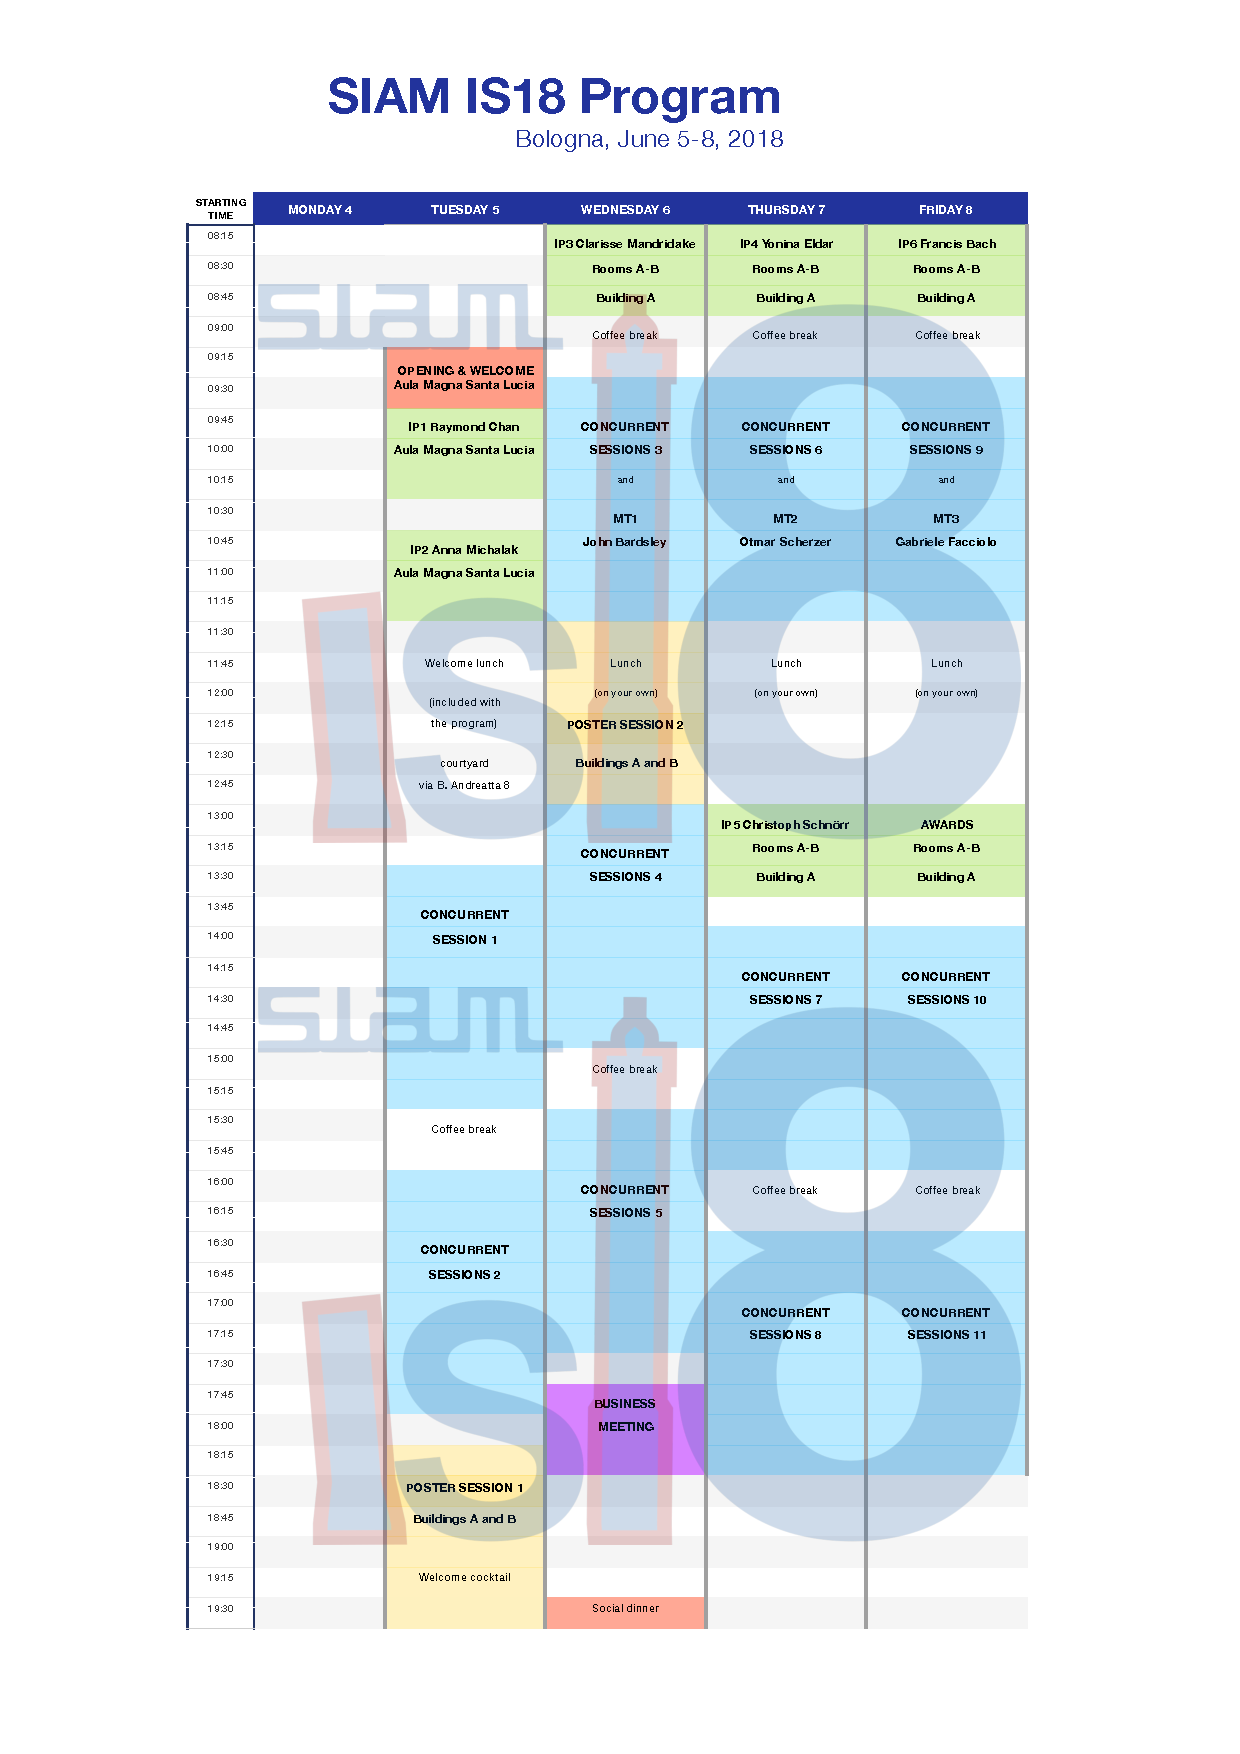
\includegraphics[scale=0.6]{program_table.pdf}
%
%
\end{document}
